\documentclass[a4paper]{article}

%% Language and font encodings
\usepackage[british]{babel} % set babel to british rather than american
\usepackage[utf8]{inputenc} % utf8 support in source code
\usepackage{lmodern}
\usepackage[T1]{fontenc} % better support for special characters in pdf but messes up title fonts, can be fixed by installing the debian package cm-super
\usepackage{textcomp}

%% Sets page size and margins
\usepackage[a4paper,top=3cm,bottom=2cm,left=3cm,right=3cm,marginparwidth=1.75cm]{geometry}

\usepackage{lineno}
\linenumbers

\usepackage{authblk}

\usepackage{mathtools} % math packages
\usepackage{amsfonts}
\usepackage{amssymb}
\usepackage{physics}
\usepackage[version=4]{mhchem}
\usepackage{tabu}
\usepackage{booktabs} % fancy tables

\usepackage{afterpage}

\usepackage{siunitx}
\sisetup{separate-uncertainty=true}
\DeclareSIUnit\radlen{\text{\ensuremath{X_{\mathrm{0}}}}}
\DeclareSIUnit\clight{\text{\ensuremath{c}}} % remove 0 subscript from speed of light

\usepackage{graphicx}
\graphicspath{{./Figures/}}
\usepackage{microtype}   
\usepackage{soul}

\usepackage[autostyle]{csquotes} % recommended by biblatex
\usepackage{xpatch} % recommended by biblatex
\usepackage[backend=biber, giveninits, sorting=none, style=numeric-comp]{biblatex} % much more flexible than BibTeX
\addbibresource{main.bib}

\newcommand*{\m}{\mathrm}


\title{ArgonCube in the DUNE Near Detector}

\author[3]{J.~Asaadi}
\author[2]{D.~A.~Dwyer}
\author[1]{A.~Ereditato}
\author[1]{D.~Goeldi}
\author[1]{P.~P.~Koller}
\author[4,5]{K.~S.~McFarland}
\author[2]{C.~M.~Marshall}
\author[1]{J.~R.~Sinclair\thanks{Corresponding author: james.sinclair@lhep.unibe.ch}}
\author[1]{C.~Wilkinson}

\affil[1]{Albert Einstein Center for Fundamental Physics, Laboratory for High Energy Physics,  University of Bern, 3012 Bern, Switzerland}
\affil[2]{University of California and Lawrence Berkeley National Laboratory, Berkeley, California 94720, USA}
\affil[3]{Department of Physics, The University of Texas at Arlington, Arlington, Texas 76019, USA}
\affil[4]{Fermi National Accelerator Laboratory, Batavia, Illinois 60510, USA}
\affil[5]{University of Rochester, Rochester, New York 14627 USA}

\renewcommand\Authands{ and }


\begin{document}
	\maketitle
	
	
\begin{abstract}
To allow LArTPCs to operate in the high-multiplicity near detector environment of DUNE, a new type of LArTPC has been proposed - ArgonCube(ArC).
ArC is a modular design with the detector volume segmented into an number of TPCs sharing a common cryostat, using a novel pixelated charge readout that enables the full 3D tracking capabilities of LArTPCs. 
The DUNE ND Conceptual Design group has requested studies from ArgonCube to demonstrate its expected performance, and to help identify the optimal choice of complimentary low-density tracker.
This document presents the results of these studies.    
\end{abstract}

\section{Task List from the DUNE ND WG}

This is a working document that will form the basis of a CDR, it will be updated with new results as studies develop. 

There is no established time-line for obtaining the answers for the LAr detector. 
While all agree that a LAr detector should be included, there remain a number of important technical questions that need to be answered before the collaboration is able to make a decision.
It is important that the following questions are addressed:

\begin{enumerate}
	\item Can the LAr detector handle high rates?
	\item The feasibility of the pixel readout needs to be demonstrated.
	\item What is the optimal height of the active volume based on scientific needs?
	\item Can neutrino-electron elastic scattering be measured?
	\item What size is needed for hadron containment?
	\item Is a side muon spectrometer needed?
	\item What is the statistics in the fiducial volume(FV)?
	\item What is the muon acceptance for neutrino interactions in LAr for different tracker options?
	\item What are muon/electron momentum resolution and scale error?
	\item Can the LAr detector measure neutrons?
\end{enumerate}

Points 1,2, and 3 are of higher priority.
The feasibility of the pixel readout needs to be demonstrated before any comment can be made on the ability of ArgonCube to handle the high rate.
A study of hadron containment will be used to identify optimal detector dimensions, the event rate in the FV will then be found for these dimensions. 

We will begin by introducing ArgonCube, since an understanding of the detector concept is needed for the requested studies.
	
\section{Introduction} \label{sec:Intro}

At the near detector, only \SI{574}{\metre} from the target, the beam intensity, $\order{\SI{1}{\mega\watt}}$, corresponds to $\order{0.1}$~events~per~tonne~per~beam~spill~\cite{DUNE2,DUNE3}.
To minimise detector response uncertainties between the near and far, it would be ideal to have a LArTPC component of the DUNE near detector complex.
Unfortunately, traditional LArTPCs are not suitable for near detector environments.
Since their evolution from gaseous TPCs~\cite{TPC,LArIonize,LArTPC}, the charge readout for LArTPCs has been achieved with two or more projective wire planes. 
Projective wire readouts have been successfully demonstrated in a number of experiments~\cite{icarus,argonute,uboner}, however they introduce intrinsic ambiguities in event reconstruction~\cite{ambiguous}. 
The ambiguities are due to reconstructing complex 3D shapes with a limited number of 2D projections, and are particularly problematic if tracks are aligned parallel to the wire plane, or multiple events overlap in drift direction.    
LArTPCs are slow detectors with a drift speed of \SI{2.1}{\milli\metre\per\micro\second} at \SI{1}{\kilo\volt\per\centi\metre}~\cite{protoLASER}, making event pile-up a problem for projective wire readouts in high-multiplicity near detector environments.
It is possible to increase voltages beyond \SI{1}{\kilo\volt\per\centi\metre}\cite{breakdown_16, latex}, however it is both safer and simpler to overcome pile-up with a charge readout free from ambiguities and shorter drift distances. 
For this reason, ArgonCube is being developed. 

Modularity reduces pile-up and allows for shorter drift-times and thus slackens the requirements on argon purity and high voltage (HV).
A modular detector furthermore reduces event pile-up because the acquisition time is reduced to the size of one half module.
Finally, trigger purity profits from a modular approach because scintillation light is contained within each module, allowing for a localised trigger.

\begin{figure}[tbp]
	\centering
	\includegraphics[width=\textwidth]{Figures/Normal-Module-4K_labelled}
	\caption[ArgonCube module engineering drawing]{%
		Cutaway drawing of a \SI{0.67 x 0.67 x 1.81}{\metre} ArgonCube module for the $2\times2$ module prototype at Bern.
	}
	\label{fig:ac_module}
\end{figure}

ArC is made of self-contained TPC modules sharing a common cryostat.
A module is made of a rectangular box with a square footprint and the height required by physics goals and/or sensitivity constraints.
The top flange is made of stainless steel while the side walls are made from \SI{1}{\centi\metre} G10 sheets.

G10's EM radiation length ($X_{\m{0}} = \SI{19.4}{\centi\metre}$) and hadronic interaction length ($\lambda_{\m{int}} = \SI{53.1}{\centi\metre}$)~\cite{pdg_g10} are both comparable to LAr, $1.4\times10^{-1}$~m and $8.37\times10^{-1}$~m respectively.
This makes G10 structures in LAr almost transparent for passing particles allowing for a performance comparable to a monolithic detector.
The module walls produce gaps in particle tracks traversing multiple modules similar to dead wires in classic LArTPC readouts.
Algorithms to join such segmented tracks already exist~\cite{pandora}.
However, a detailed study of the influence of module walls on reconstruction efficiency still needs to be performed.
At the same time, inactive volume is drastically reduced compared to a monolithic design due to the comparably low cathode voltage.
The modules are placed side-by-side in a LAr bath where they can be extracted and reinserted as needed.
Pressure inside the modules is kept close to the bath pressure putting almost no hydrostatic force on the module walls.
Purity of the LAr is maintained within each module by means of a recirculation system.
As a result, the argon surrounding the modules needs not meet as stringent purity requirements as the argon inside.
Under normal operation conditions all modules are inserted with only clearance distances between modules.
A drawing of an ArC module is shown in Figure~\ref{fig:ac_module}.

During module insertion and extraction the argon flow is controlled by hydrostatic check valves located at the module bottom.
They require a minimal differential pressure to open.
Purity inside to modules is maintained by means of continuous LAr recirculation through oxygen traps.
The dirty argon is sucked in at the module top and then pushed through the oxygen traps.
The clean argon is first routed through a heat exchanger, located below the module inside the outer bath, for cooling and then re-enters the module at the bottom.
For optimal heat transport the argon flow is directed along the cold electronics.
To prevent dirty argon from the bath entering the modules their interior is held at a slight overpressure, just below the opening pressure of the check valves.
Cooling power to the bath is supplied by cryocoolers located in unistrumented volumes at the side of the detector called service volumes.

There are two slightly different options for the recirculation system.
To maximise module autonomy each module can be equipped with its own oxygen trap and LAr pump.
Drawbacks of this are the very high cost of pumps and the additional dense material close to the detector volume.
Additionally, the DUNE ND complex is planned to consist of a magnetised detector besides ArC.
The resulting magnetic stray fields might interfere with the electric motors of LAr pumps on top of the modules.
Using a shared recirculation circuit is more economic but reduces module autonomy.
An external system comprising pumps and oxygen traps can be located outside the argon bath (and potential magnetic stray fields), connected to the modules via tubes.

One big problem that can be solved by a modular design is the high cathode voltage required for large monolithic detectors, and the resulting stored energy.
As each module contains two TPCs independent of all other modules, the required cathode potential only depends on the module size, not the detector size.
To minimise the cathode voltage the drift field is applied along one of the short edges of a module.
In addition, the module is split in two half TPCs by the cathode, reducing the voltage by a factor of two.
Thus, for a module footprint of \SI{1 x 1}{\metre} and an electric field of \SI{1}{\kilo\volt\per\centi\metre} a cathode potential of only \SI{50}{\kilo\volt} is required.
Operating a LArTPC at this voltage is challenging but feasible without a prohibitive loss in active volume~\cite{AT}.
The HV is brought into the module using a commercially available feedthrough.
To replace field-shaping rings an improved solution with a continuous resistive-plane field cage formed of carbon-impregnated Kapton is under investigation.
This will provide a very homogeneous field paired with simple mechanics.

The high rates present in an ND environment will lead to a significant amount of event pile-up.
Disentangling the individual neutrino events requires a highly capable charge readout.
Solving this task with a projective wire readout is more than doubtful.
To enable true 3D tracking the modules are equipped with a pixelated charge readout very similar to the one described in~\cite{pixels}.
Pixelated anode planes are located on the two module walls parallel to the cathode.
The bespoke LArPix cryogenic electronics, described in Section~\ref{sec:pix}, are used to digitise the signals in cold to achieve unambiguous 3D information.

One of the main challenges for the light readout are again the high rates faced by an ND.
To get proper timing for the third spatial coordinate scintillation signals need to be correctly matched to charge signals (flash matching).
Furthermore, attenuation due to Rayleigh scattering,$6.6\times10^{-1}$~m, becomes a problem for large detectors.
Both problems are greatly alleviated by using an opaque cathode and module walls, containing the scintillation light inside a single module half (TPC).
Therein, pile-up is reduced due to the smaller volume.
Having a position-resolving light readout helps as well.
However, a modular TPC introduces a new challenge: The dead spaces in between adjacent TPCs has to be minimized because they introduce gaps in the recorded event topologies accompanied by lost energy.
Therefore, ArC modules are instrumented with the ArCLight light collection system~\cite{arclight}.
With its light trap design it allows light collection from a large area with a minimal dead volume.
The location of the SiPMs at the edges of a dielectric sheet makes most of the light detector immune to electric fields.
Splitting ArCLight into several horizontal strips stacked vertically gives spatial resolution in the vertical direction.
ArCLight sheets are mounted in between cathode and anode, parallel to the field cage, with the SiPMs directly attached to the charge readout PCB.
The additional dead volume of a few \si{\milli\metre} is similar to the one caused by the charge readout in perpendicular direction.

\section{Pixel Feasibility}

This section is split into three parts, it will introduce the initial prototype pixel readout at Bern~\cite{pixels} followed by test beam studies of this technology at FNAL. Finally the status of the bespoke pixel ASICs~\cite{larpix} will be discussed.
    
\subsection{Analogue Multiplexing}

To make use of existing wire-readout ASICs a Region Of Interest (ROI)-based analogue multiplexing scheme had to be implemented. 
The scheme divides the pixels into a number of Regions Of Interest (ROIs).
Each ROI is defined as the pixels contained within a single inductive focusing grid.
All pixels at the same coordinate inside each of the ROIs are connected to the same DAQ channel, i.e. only one DAQ channel connects all the pixels in the top left corners of all ROIs, and so on.

Pixel signals are then associated to an induction signal on the ROI grid as follows. 
If there is a signal on a certain pixel DAQ channel, the position inside the ROI is known but not which ROI.
By combining the inductive bipolar pulse on the ROI grid with any simultaneous collection pulses from the pixels, it is possible to disentangle the true position.
The drawback of this approach is that it is not free from ambiguities; it fails for multiple simultaneous hits when it is impossible to say which pixel pulse belongs to which ROI pulse.
Ambiguous hits are flagged as pixel signals corresponding to multiple ROI signals, which can be disentangled later using reconstruction tools.
 
Ideally, every pixel would be read out and the signals then digitally multiplexed, requiring bespoke pixel ASIC capable of cold amplification and digitisation for many channels.
Such ASICs are being developed by LBNL, and will be described in Section~\ref{sec:pix}.

\subsection{Initial Prototypes}

The pixelated anode plane, shown in Figure~\ref{fig:viper_pixies}, was produced as a conventional PCB.
The pixelated area is \SI{100}{\milli\metre} across, the pixels are formed of \SI{900}{\micro\metre} vias with a pitch of \SI{2.54}{\milli\metre}.
An inductive focusing grid surrounds the pixels, it is made from \SI{152.4}{\micro\metre} copper traces split into 28 regions.
There are \num{6 x 6} pixels per region, giving a total of 1008 pixels. 

\begin{figure}[tbp]
	\centering
	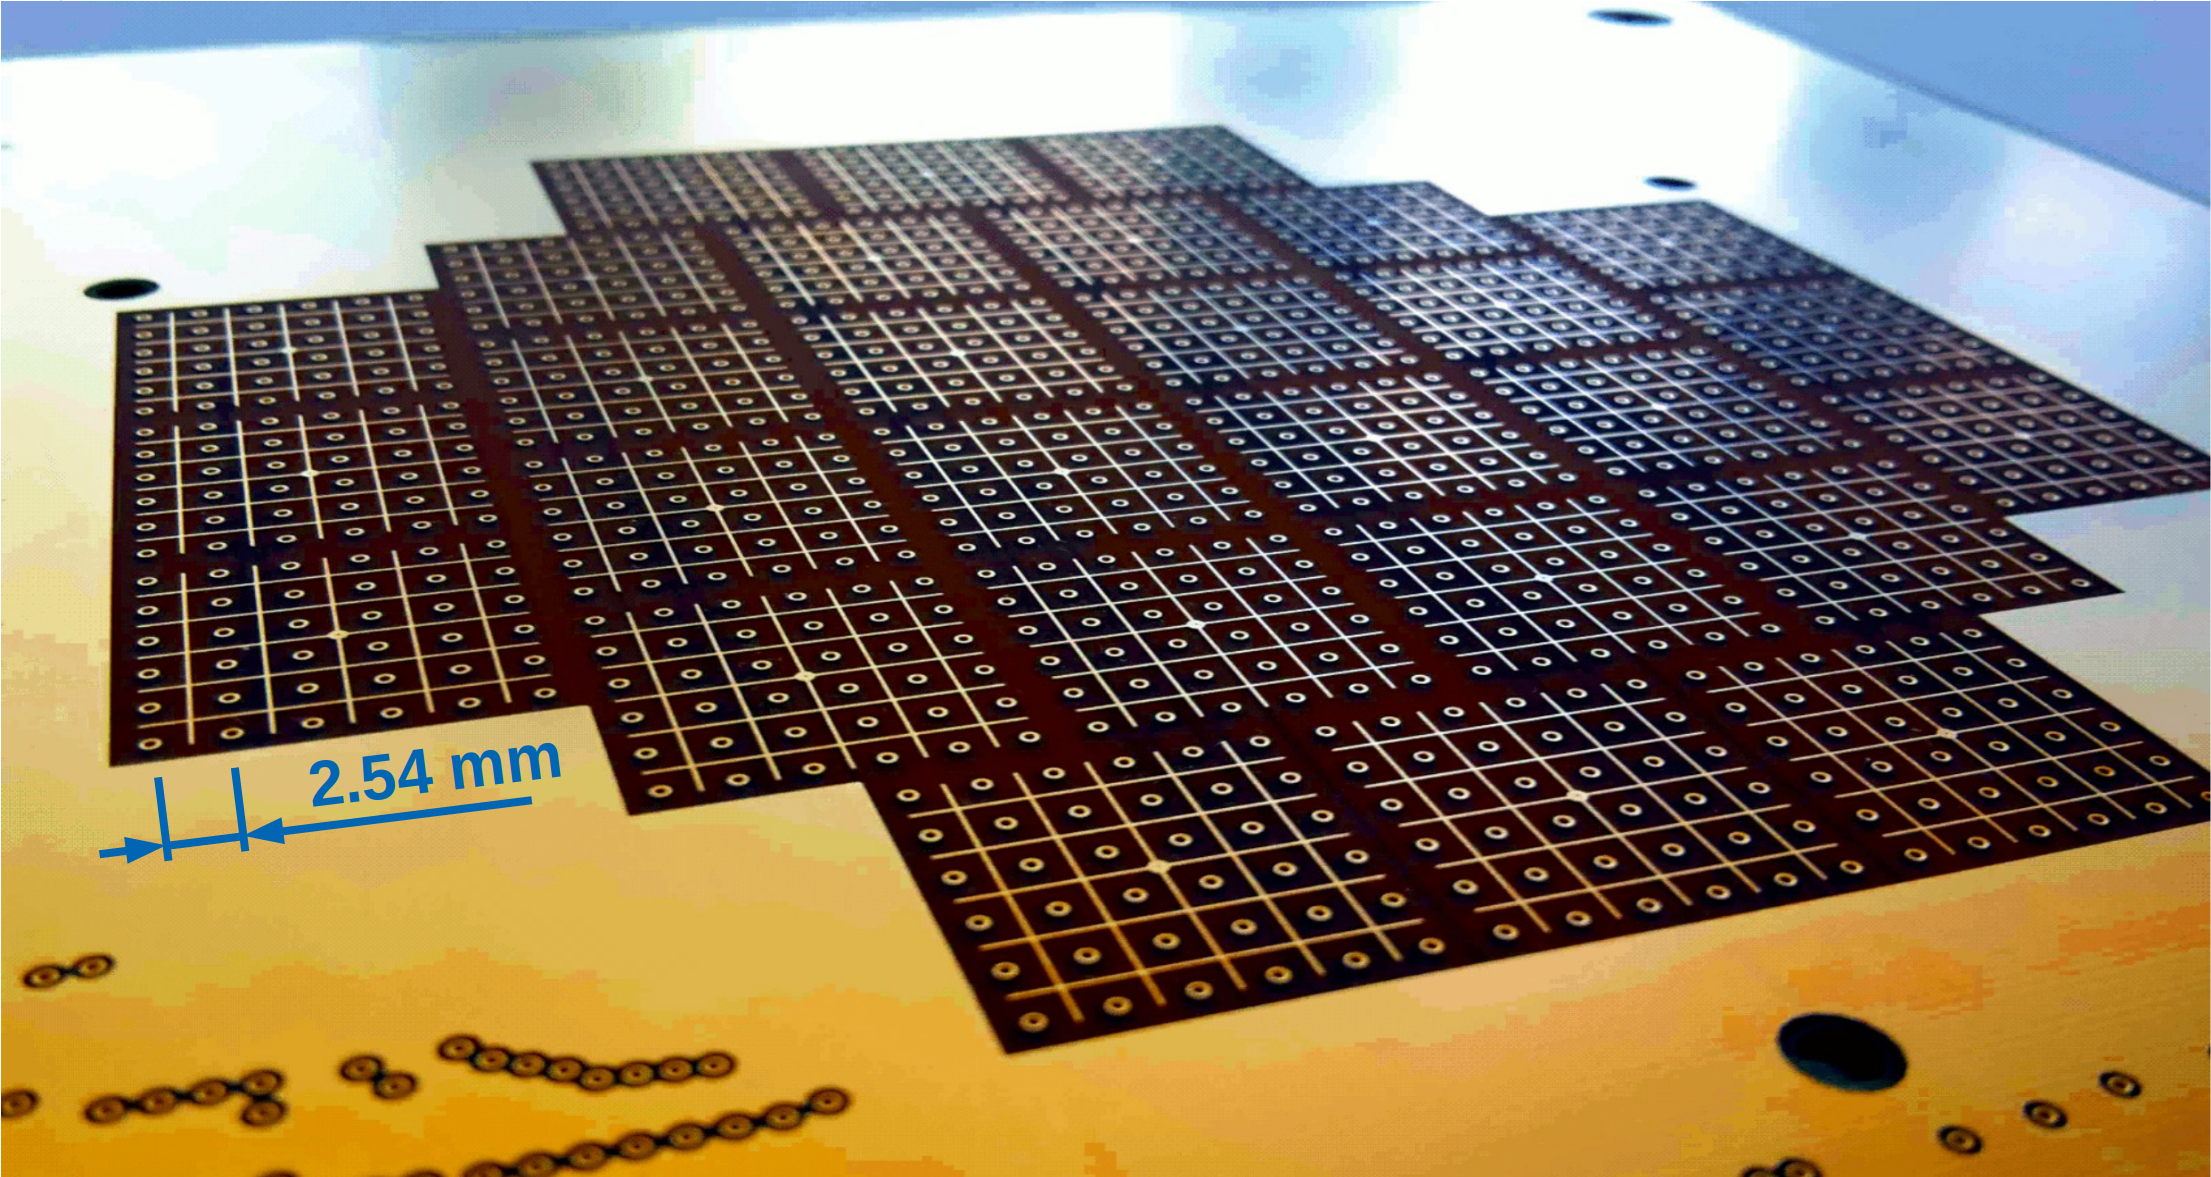
\includegraphics[width=\textwidth]{Figures/pixies}
	\caption[Pixel demonstrator readout plane]{%
		First (high-capacitance) version of the pixelated anode PCB.
		The pixelated readout area is \SI{100}{\milli\metre} in diameter.
		Each charge collection pixel is a \SI{900}{\micro\metre} via, at a pitch of \SI{2.54}{\milli\metre}.
		Inductive focusing grids formed of \SI{152.4}{\micro\metre} copper traces surround the pixels.
		There are \num{28} inductive focusing grids with \num{36} pixels per region, a total of \num{1008} pixels.
	}
	\label{fig:viper_pixies}
\end{figure}

The pixel demonstrator TPC, shown in Figures~\ref{fig:viper_v1per}, is cylindrical with an inner diameter of \SI{101}{\milli\metre} and a \SI{590}{\milli\metre} drift length. 
The light readout was provided by cold SiPMs coupled via WLS fibres to TPB coated light collectors between the field cage. 
The TPC operated with a drift field of \SI{1}{\kilo\volt\per\centi\metre}, corresponding to a total drift time of \SI{281}{\micro\second} at \SI{2.1}{\milli\metre\per\micro\second}~\cite{protoLASER}.

\begin{figure}[tbp]
	\centering
	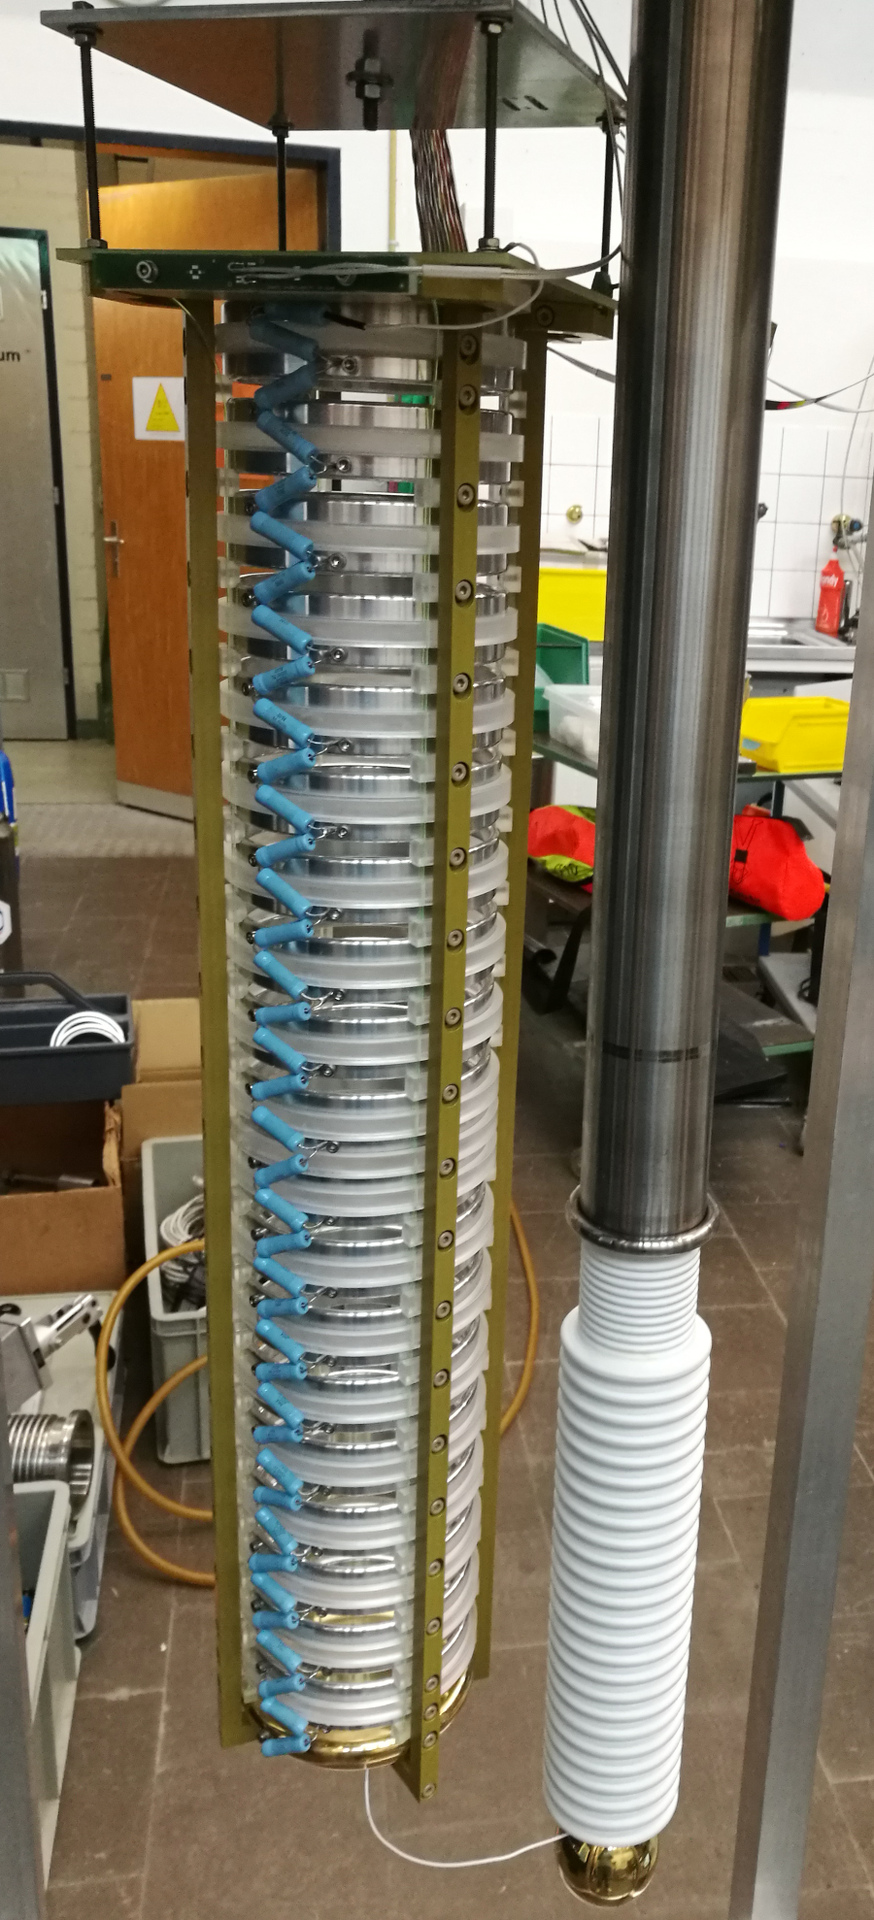
\includegraphics[width=.25\columnwidth]{Figures/viper_original}
	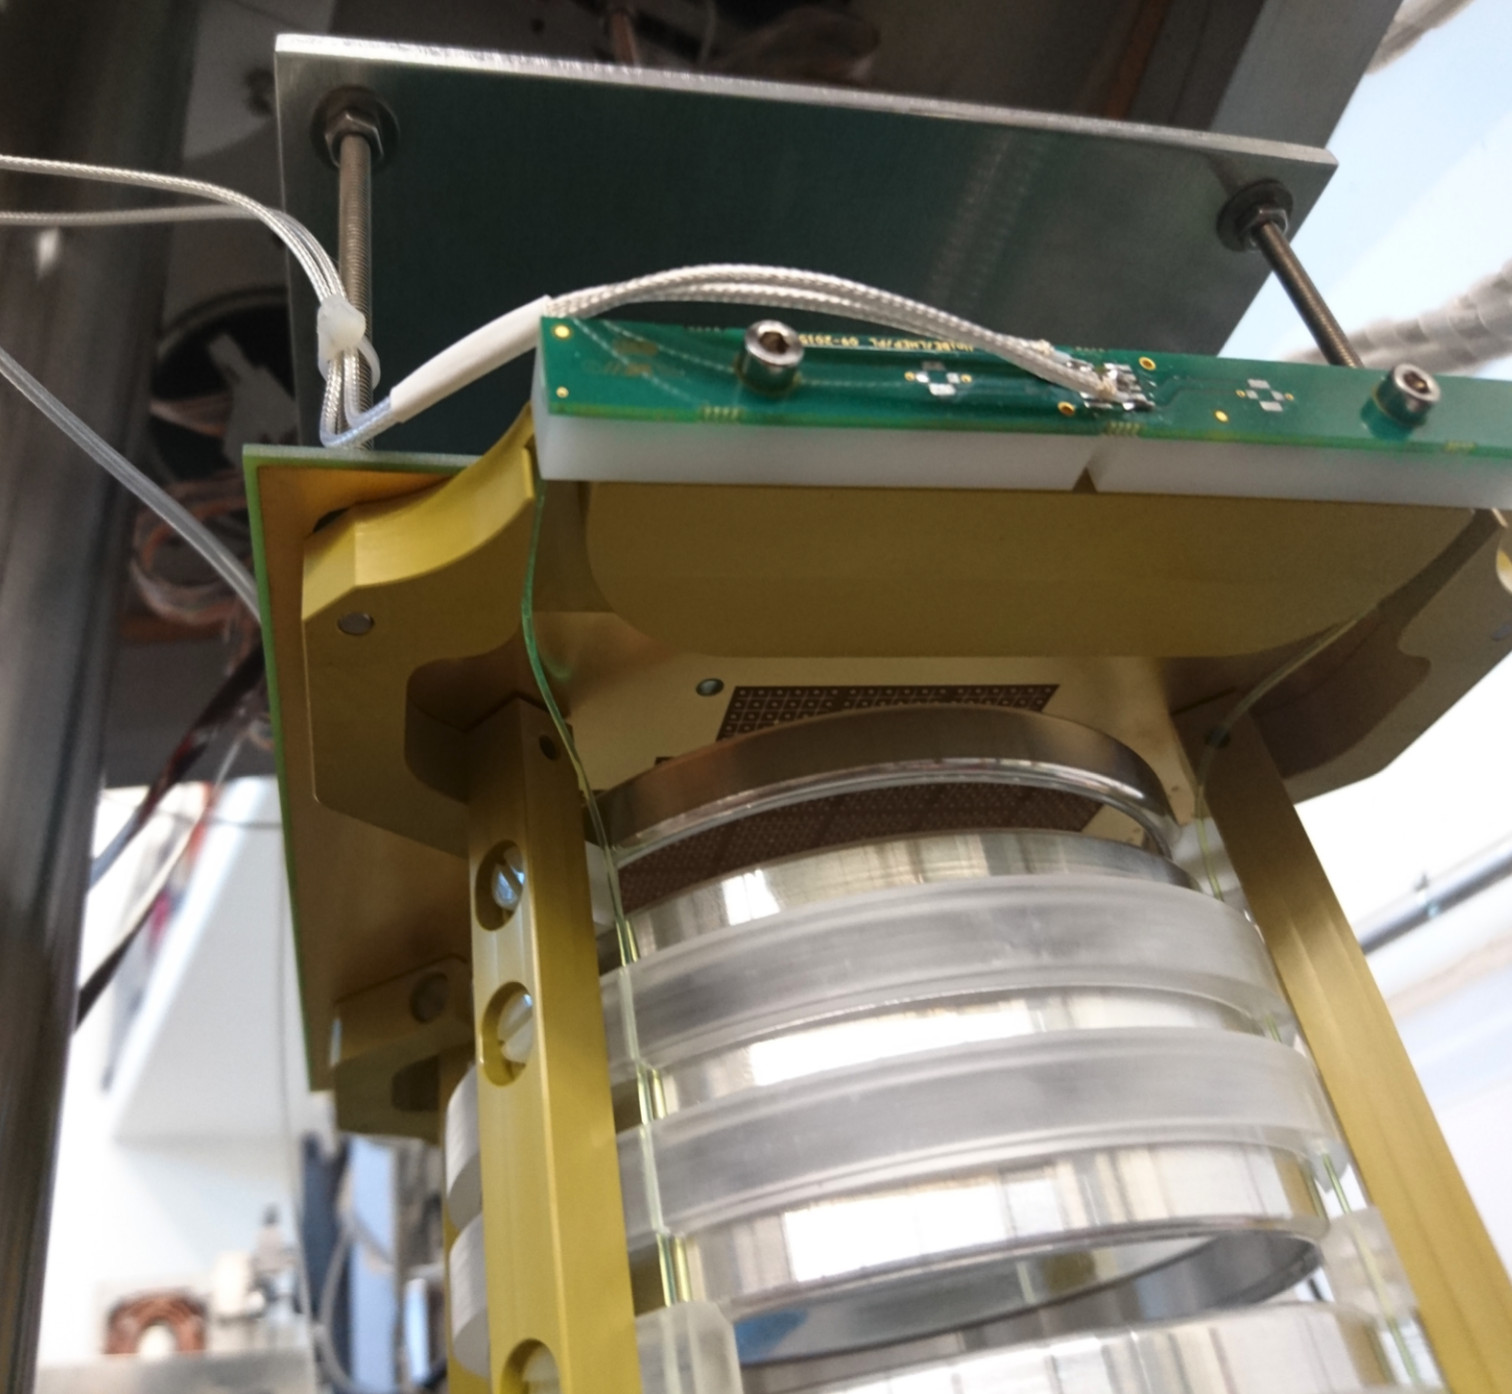
\includegraphics[width=.6\columnwidth]{Figures/viper_sipm}
	\caption[Pixel demonstrator close-up]{%
		Left: Photograph of the  pixel demonstrator TPC at Bern, with the HV feedthrough.
		Right: Close-up of the light collection system, showing WLS fibres coupling the SiPM to the TPB-coated light guides.
	}
	\label{fig:viper_v1per}
\end{figure}

\subsubsection{Signal to Noise Ratio}

To assess the Signal to Noise Ratio (SNR) dedicated noise data was taken employing a \SI{5}{\hertz} random trigger.
For the \num{2000} recorded events, all pixel and ROI channels were combined respectively and filled into amplitude distribution histograms.
The standard deviation of the two noise distributions was then calculated by fitting a Gaussian.
This value was used to calculate the noise for pixel and ROI channels according to
\begin{equation}
\m{SNR} = \frac{S}{\sigma}\,\m{,}
\label{eq:snr}
\end{equation}
where $\sigma$ is the noise standard deviation from the Gaussian fit and $S$ is the expected signal, which will be explained in detail below.
The resulting equivalent noise charge is \SI{1095}{\elementarycharge} for the pixel channels and \SI{982}{\elementarycharge} for the inductive ROI channels.

The signal $S$ is often taken for a Minimum-Ionising Particle (MIP) as this is at the lower end of the signal range interesting for neutrino physics.
Getting a clean MIP sample from experimental data requires a calibrated reconstruction which was not available at the time of writing.
Therefore, we estimated the MIP signal from theory assuming an energy loss of \SI{2.1}{\mega\electronvolt\per\centi\metre}~\cite{pdg}.
This can be converted to charge loss using the energy required to produce one electron-ion pair: $W_{\m{i}} = \SI{23.6}{\electronvolt\per\elementarycharge}$~\cite{NobleGasDetectors}.
Additionally, charge recombination, diffusion and attachment losses characterised by lifetime need to be taken into account.
The recombination factor was measured by both the ICARUS and ArgoNeuT collaborations~\cite{icarusReco, argoneutReco}, and found to be $R_{\m{c}} \approx 0.7$ for a drift field of $\SI{1}{\kilo\volt\per\centi\meter}$.
For a non-zero drift field, diffusion needs to be split into longitudinal and transverse components.
Using the ARGONTUBE detector in Bern~\cite{argontube}, we measured a transverse diffusion coefficient $D_{\m{T}} = \SI{5.3}{\centi\metre\squared\per\second}$ at \SI{0.25}{\kilo\volt\per\centi\metre} while Gushchin et al.~\cite{gushchin} report a value of $D_{\m{T}} = \SI{13}{\centi\metre\squared\per\second}$ at \SI{1}{\kilo\volt\per\centi\metre}.
Even using the more conservative value, this results~\cite{lngDet} in a transverse spread of
\begin{equation}
\sigma_{\m{T}} = \sqrt{2 D_{\m{T}} t} \approx \SI{0.9}{\milli\metre}\,, 
\end{equation}
for our drift time of $t = \SI{281}{\micro\second}$; a value well below the pixel pitch of $d_{\m{p}} = \SI{2.54}{\milli\metre}$.
Considering that the longitudinal component is smaller than the transverse ~\cite{lngDet}, we neglect diffusion completely for our calculations.
Finally, our lifetime of \SI{290}{\micro\second} will result in the reduction of charge by a factor of $\approx\num{0.38}$ over the full drift distance.
Combining this, we get a signal of 
\begin{equation}
S = \dv{E}{x}_{\m{MIP}} \frac{R_{\m{c}} d_{\m{p}}}{W_{\m{i}}} = \SI{15821}{\elementarycharge}\,,
\end{equation}
for a charge deposited adjacent to the readout plane, and $S = \SI{6004}{\elementarycharge}$ for a charge deposited adjacent to the cathode.

Table~\ref{tab:snr} lists the SNR values obtained from these signal values and the aforementioned measured equivalent noise charge, using Equation~\eqref{eq:snr}.

\begin{table}[htb]
	\centering
	\caption{SNR values obtained from Equation~\eqref{eq:snr} using the theoretical signal of a MIP at the readout plane or cathode, respectively combined with the average equivalent noise charge for pixel and ROI channels obtained from measurements.}
	\label{tab:snr}
	\begin{tabu} to \textwidth {llS}
		{Channel} &	{MIP at} &			{SNR} \\
		\hline
		{Pixel} &	{Readout plane} &	\num{14} \\
		{Pixel} &	{Cathode} &			\num{5.5} \\
		{ROI} &		{Readout plane} &	\num{16} \\
		{ROI} &		{Cathode} &			\num{6.1} \\
		
	\end{tabu}
\end{table}


\subsubsection{3D Track Reconstruction}
A track reconstruction toolset was developed for the 3D space points. 
This was demonstrated on crossing cosmic muon events, triggered by the cold SiPM light readout.  

Identified pulses are combined into 3D hits by matching pixels pulses to ROI pulses.
To resolve the ambiguities, a Principal Component Analysis (PCA) is applied to the 3D space points~\cite{pca}.
The basic idea is to calculate three orthogonal eigenvectors of the 3D space point cloud.
A graphic interpretation of these eigenvectors are the three axis of an ellipsoid fitted to the data points.
In case the points form a track, one of these eigenvectors will have a much higher eigenvalue than the other two.
This eigenvector is taken as an estimate for the track direction.
We resolve the ambiguities by selecting the one closest to the track estimate.
It should be noted that bespoke pixel ASICs would render this step redundant. 

The final step consists of a Kalman filter for track identification.
For this, we used the well-established GENFIT track fitting package~\cite{genfit1, genfit2}.
Ionisation losses and multiple scattering are taken into account.
The particle is assumed to be a minimum-ionising muon with an initial momentum of \SI{260}{\mega\electronvolt} in the direction of the track estimate from the PCA.
We chose a recursive algorithm capable of dealing with outliers, a so-called \emph{deterministic annealing filter}.
This works by assigning successively lower weights to outliers with each recursion step~\cite{genfit1, genfit2}.
The resulting track is shown in Figure~\ref{fig:kalman}.

\begin{figure}[htb]
	\centering
	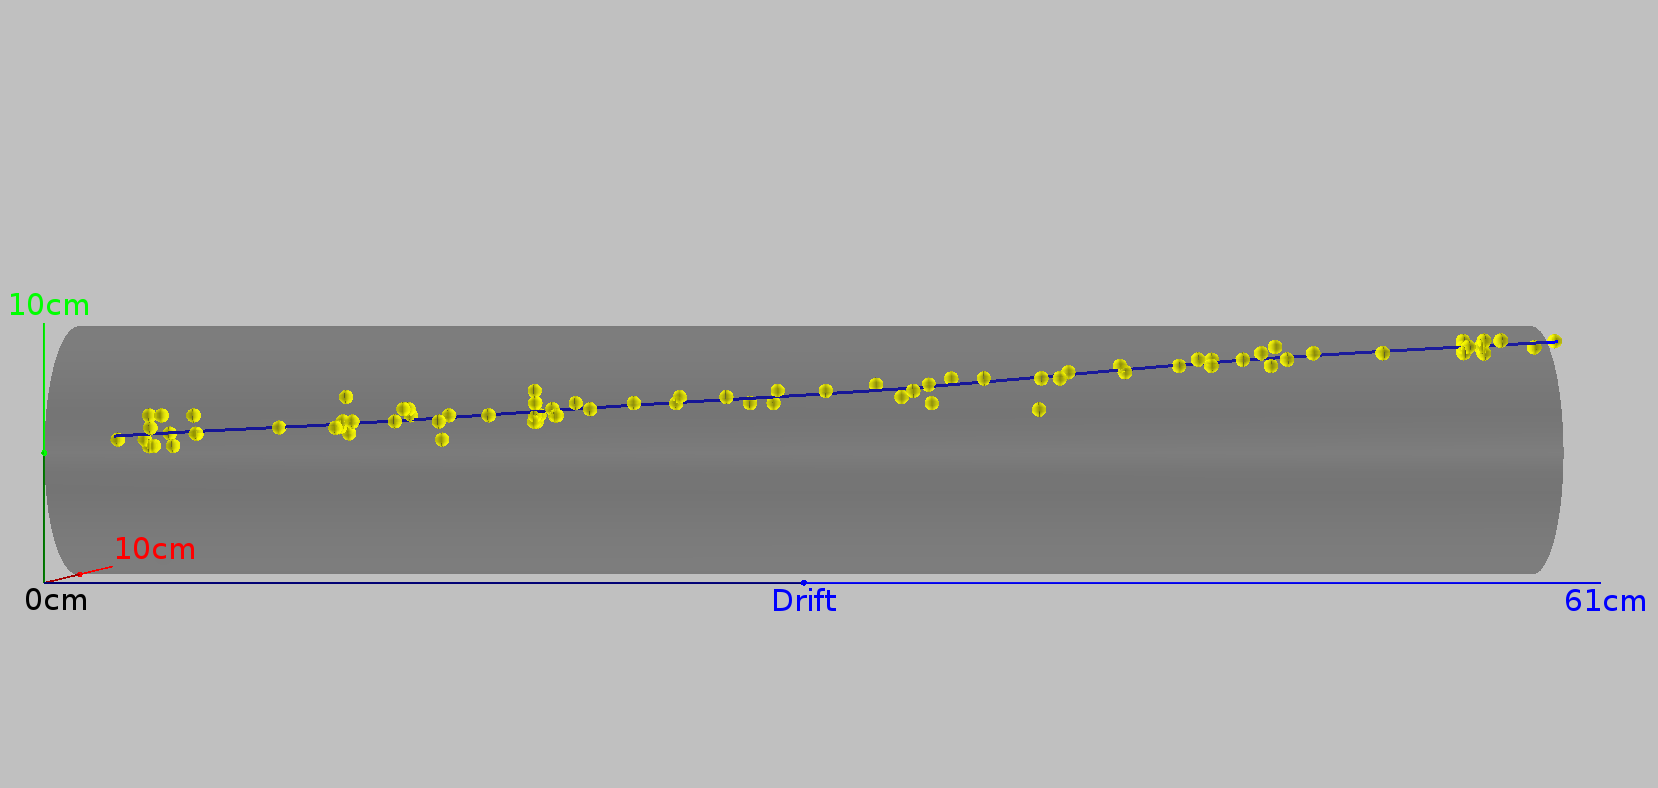
\includegraphics[width=\textwidth]{Figures/event967_kalman}
	\caption{Track fitted by the Kalman filter.
		The TPC volume is shown in faint grey.
		The passing particle is most likely a cosmic $\mu$ entering from the left.
		Drift direction is from right to left.
		The yellow points are the input to the Kalman filter, the accepted hits from the principal components analysis.
		Blue is the output, a fitted track taking into account ionisation losses and multiple scattering in LAr.}
	\label{fig:kalman}
\end{figure}

\subsection{Test Beam Studies at FNAL - PixLAr}	


\begin{figure}[tbp]
	\centering
	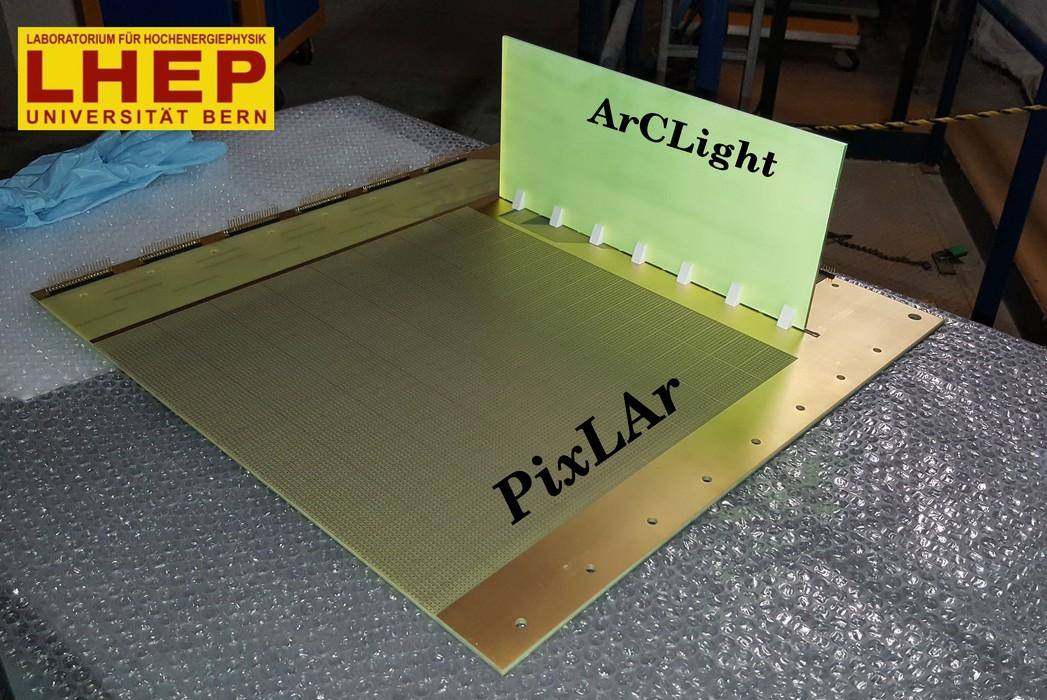
\includegraphics[width=\textwidth]{Figures/pixlar_arclight}\\
	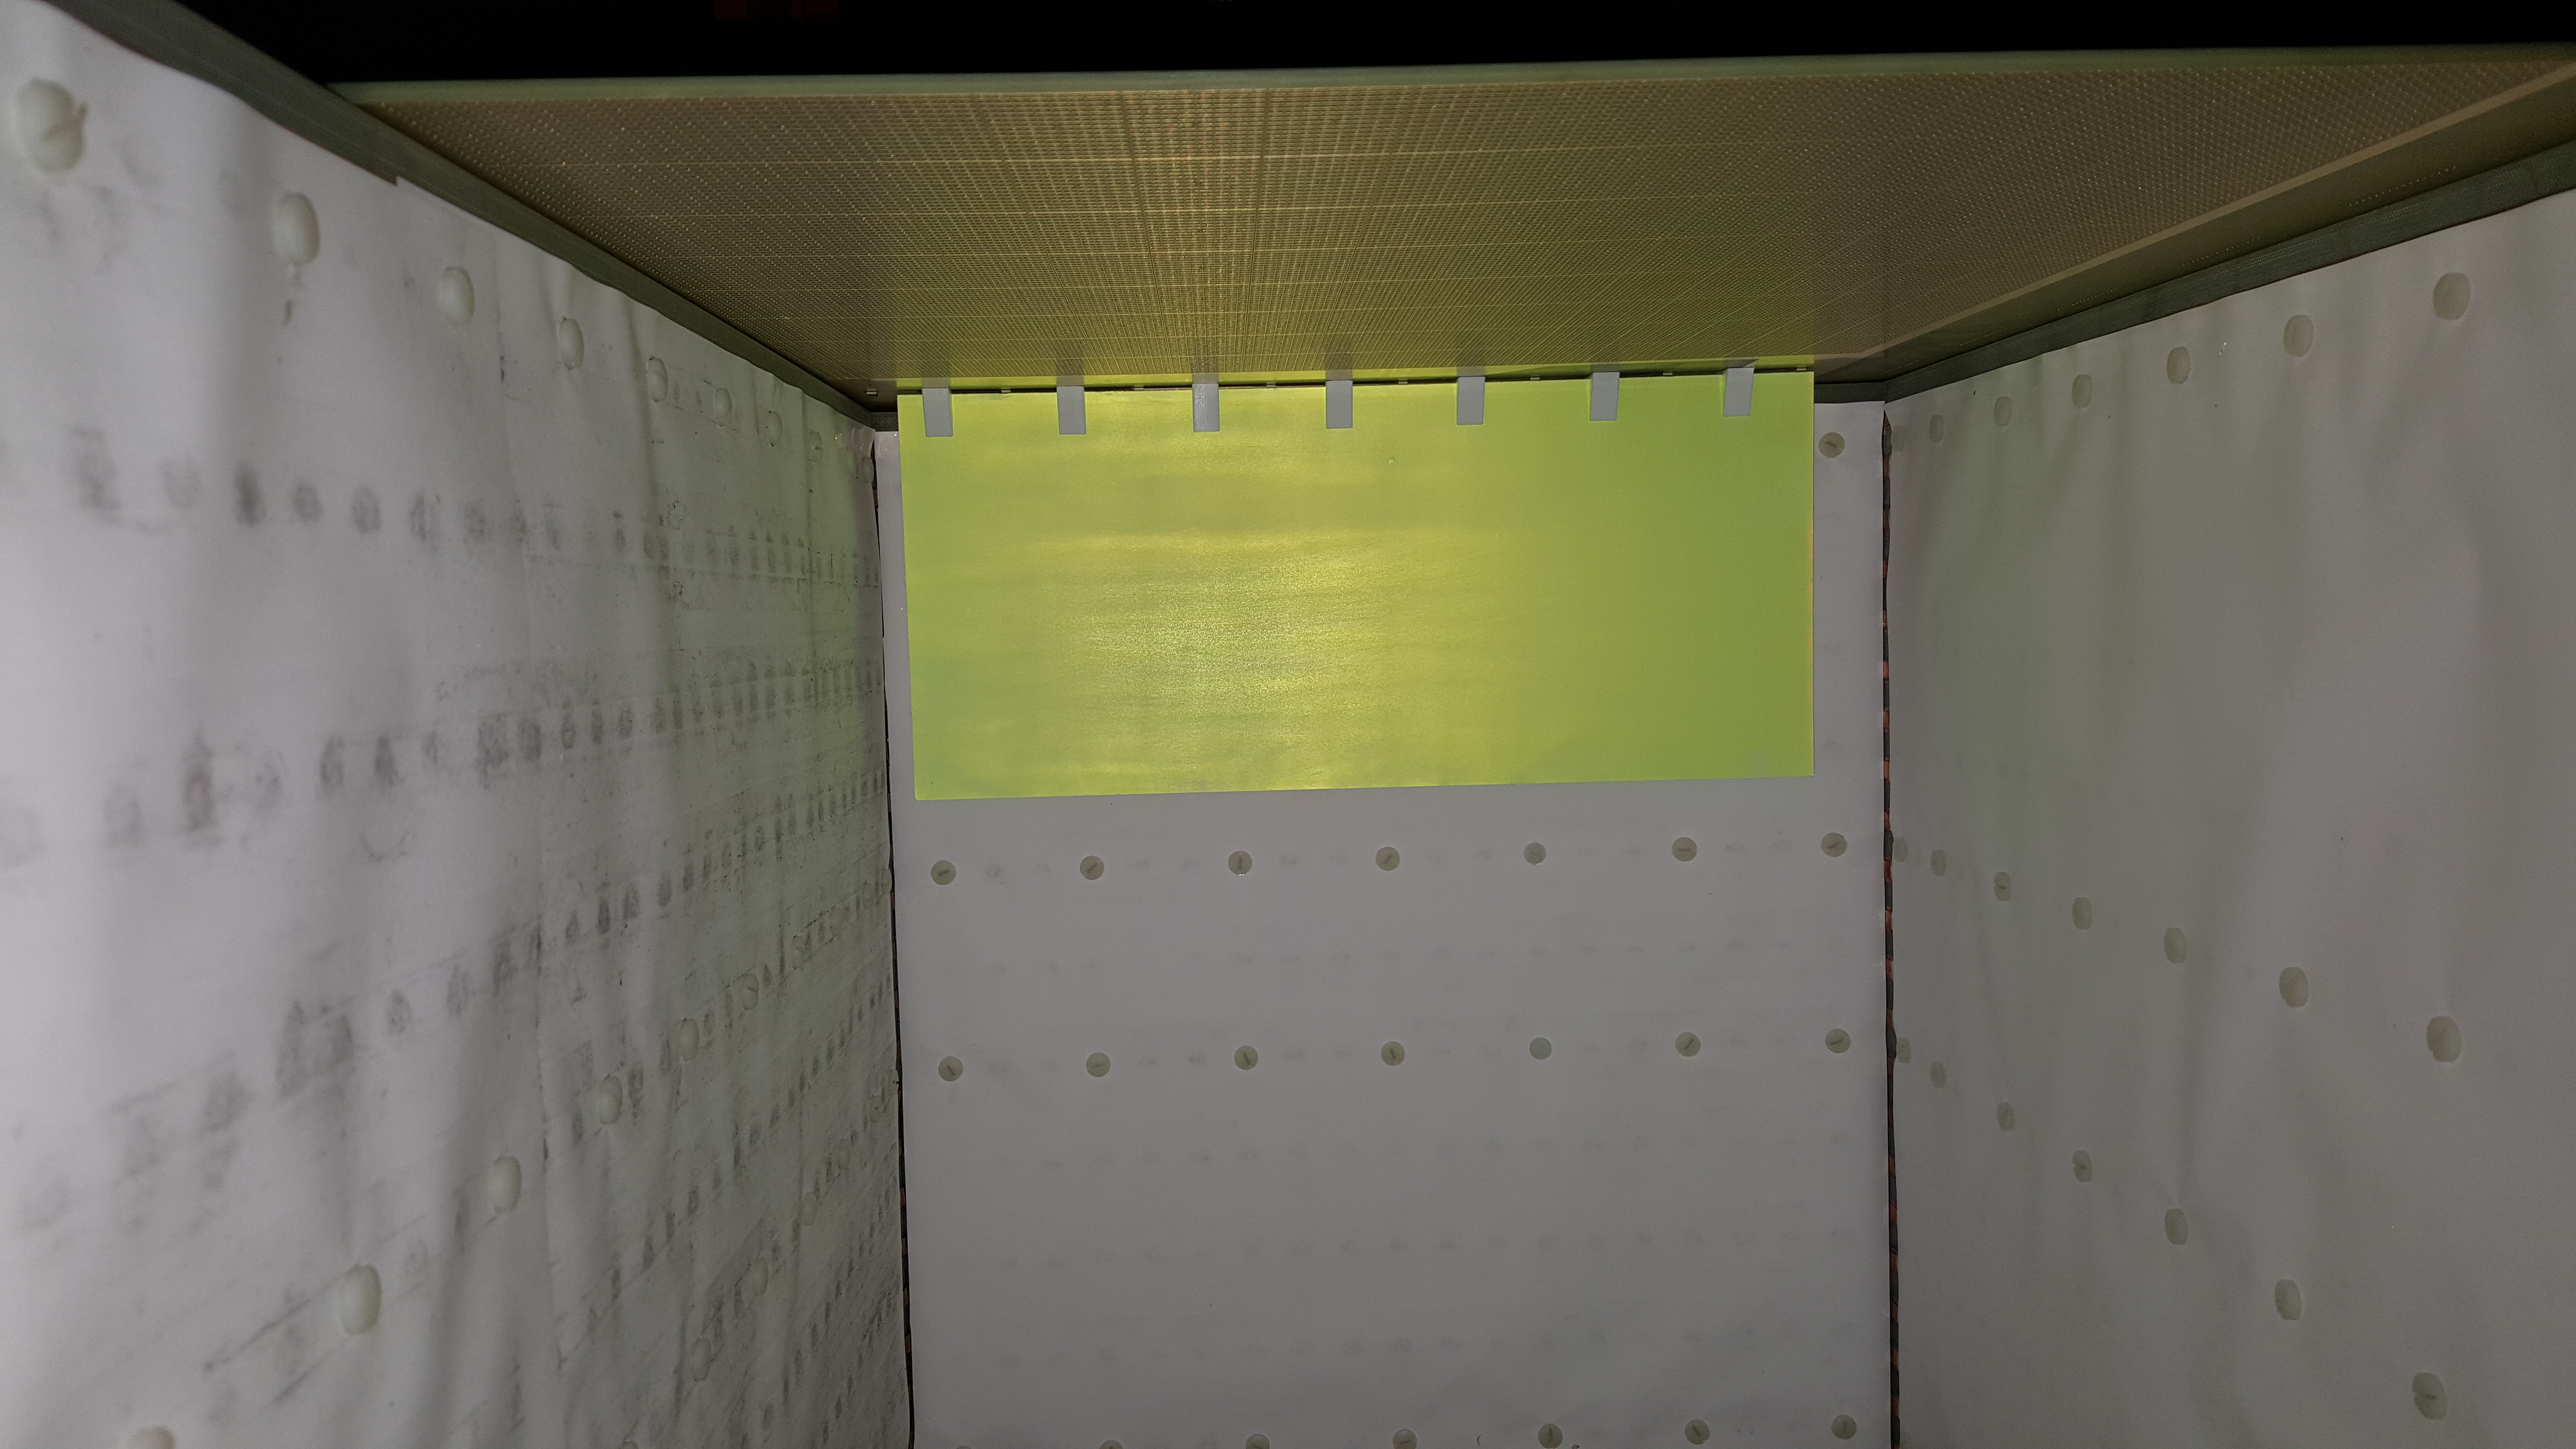
\includegraphics[width=\textwidth]{Figures/pixlar_arclight_installed}
	\caption[PixLAr half plane with attached ArCLight module]{%
		One of the two PixLAr readout half planes with the ArCLight module attached.
		The bottom picture shows the inside of the LArIAT TPC with the PixLAr ArCLight assembly installed.
	}
	\label{fig:pixlar_arclight}
\end{figure}

After successful test with cosmic muons at Bern, a scaled-up prototype of the pixel readout, employing the same multiplexing scheme, was built for a beam exposure in the LArIAT experiment~\cite{lariat} at FNAL.
LArIAT consists of the former ArgoNeut~\cite{argoneut} cryostat and TPC placed in a test beam.
The tertiary beam line produces mainly pions and protons, as well as electrons, muons, and kaons at a lower rate.
Their momentum spectrum can be tuned from \SIrange{0.2}{2.0}{\giga\electronvolt\per\clight} by means of bending magnets.
\SI{550}{\litre} of LAr are contained in a cylindrical cryostat.
It houses a TPC with \SI{47}{\centi\metre} drift length and a \SI{40 x 90}{\centi\metre} readout plane parallel to the beam direction, resulting in an active volume of \SI{170}{\litre}.
For the pixel test, called PixLAr, the original wire planes were replaced by a \num{120 x 240} pixel readout.
At \SI{3}{\milli\metre} pitch this gives an instrumented area of \SI{36 x 72}{\centi\metre}.
The readout plane had to be split into two mirror-symmetric, electrically independent half planes due to constraints from the PCB manufacturer.
Each \num{120 x 120} pixel half plane is divided into \num{8 x 15} ROI of \num{15 x 8} pixels each.
The ROI are oriented with their longer dimension parallel to the beam direction to reduce the multiplexing ambiguities.
To trigger on scintillation light one end of the TPC is equipped with a \SI{43 x 15}{\centi\metre} ArCLight module. 
Figure~\ref{fig:pixlar_arclight} shows one of the readout half planes with the ArCLight module attached.

\begin{figure}[htb]
	\centering{
		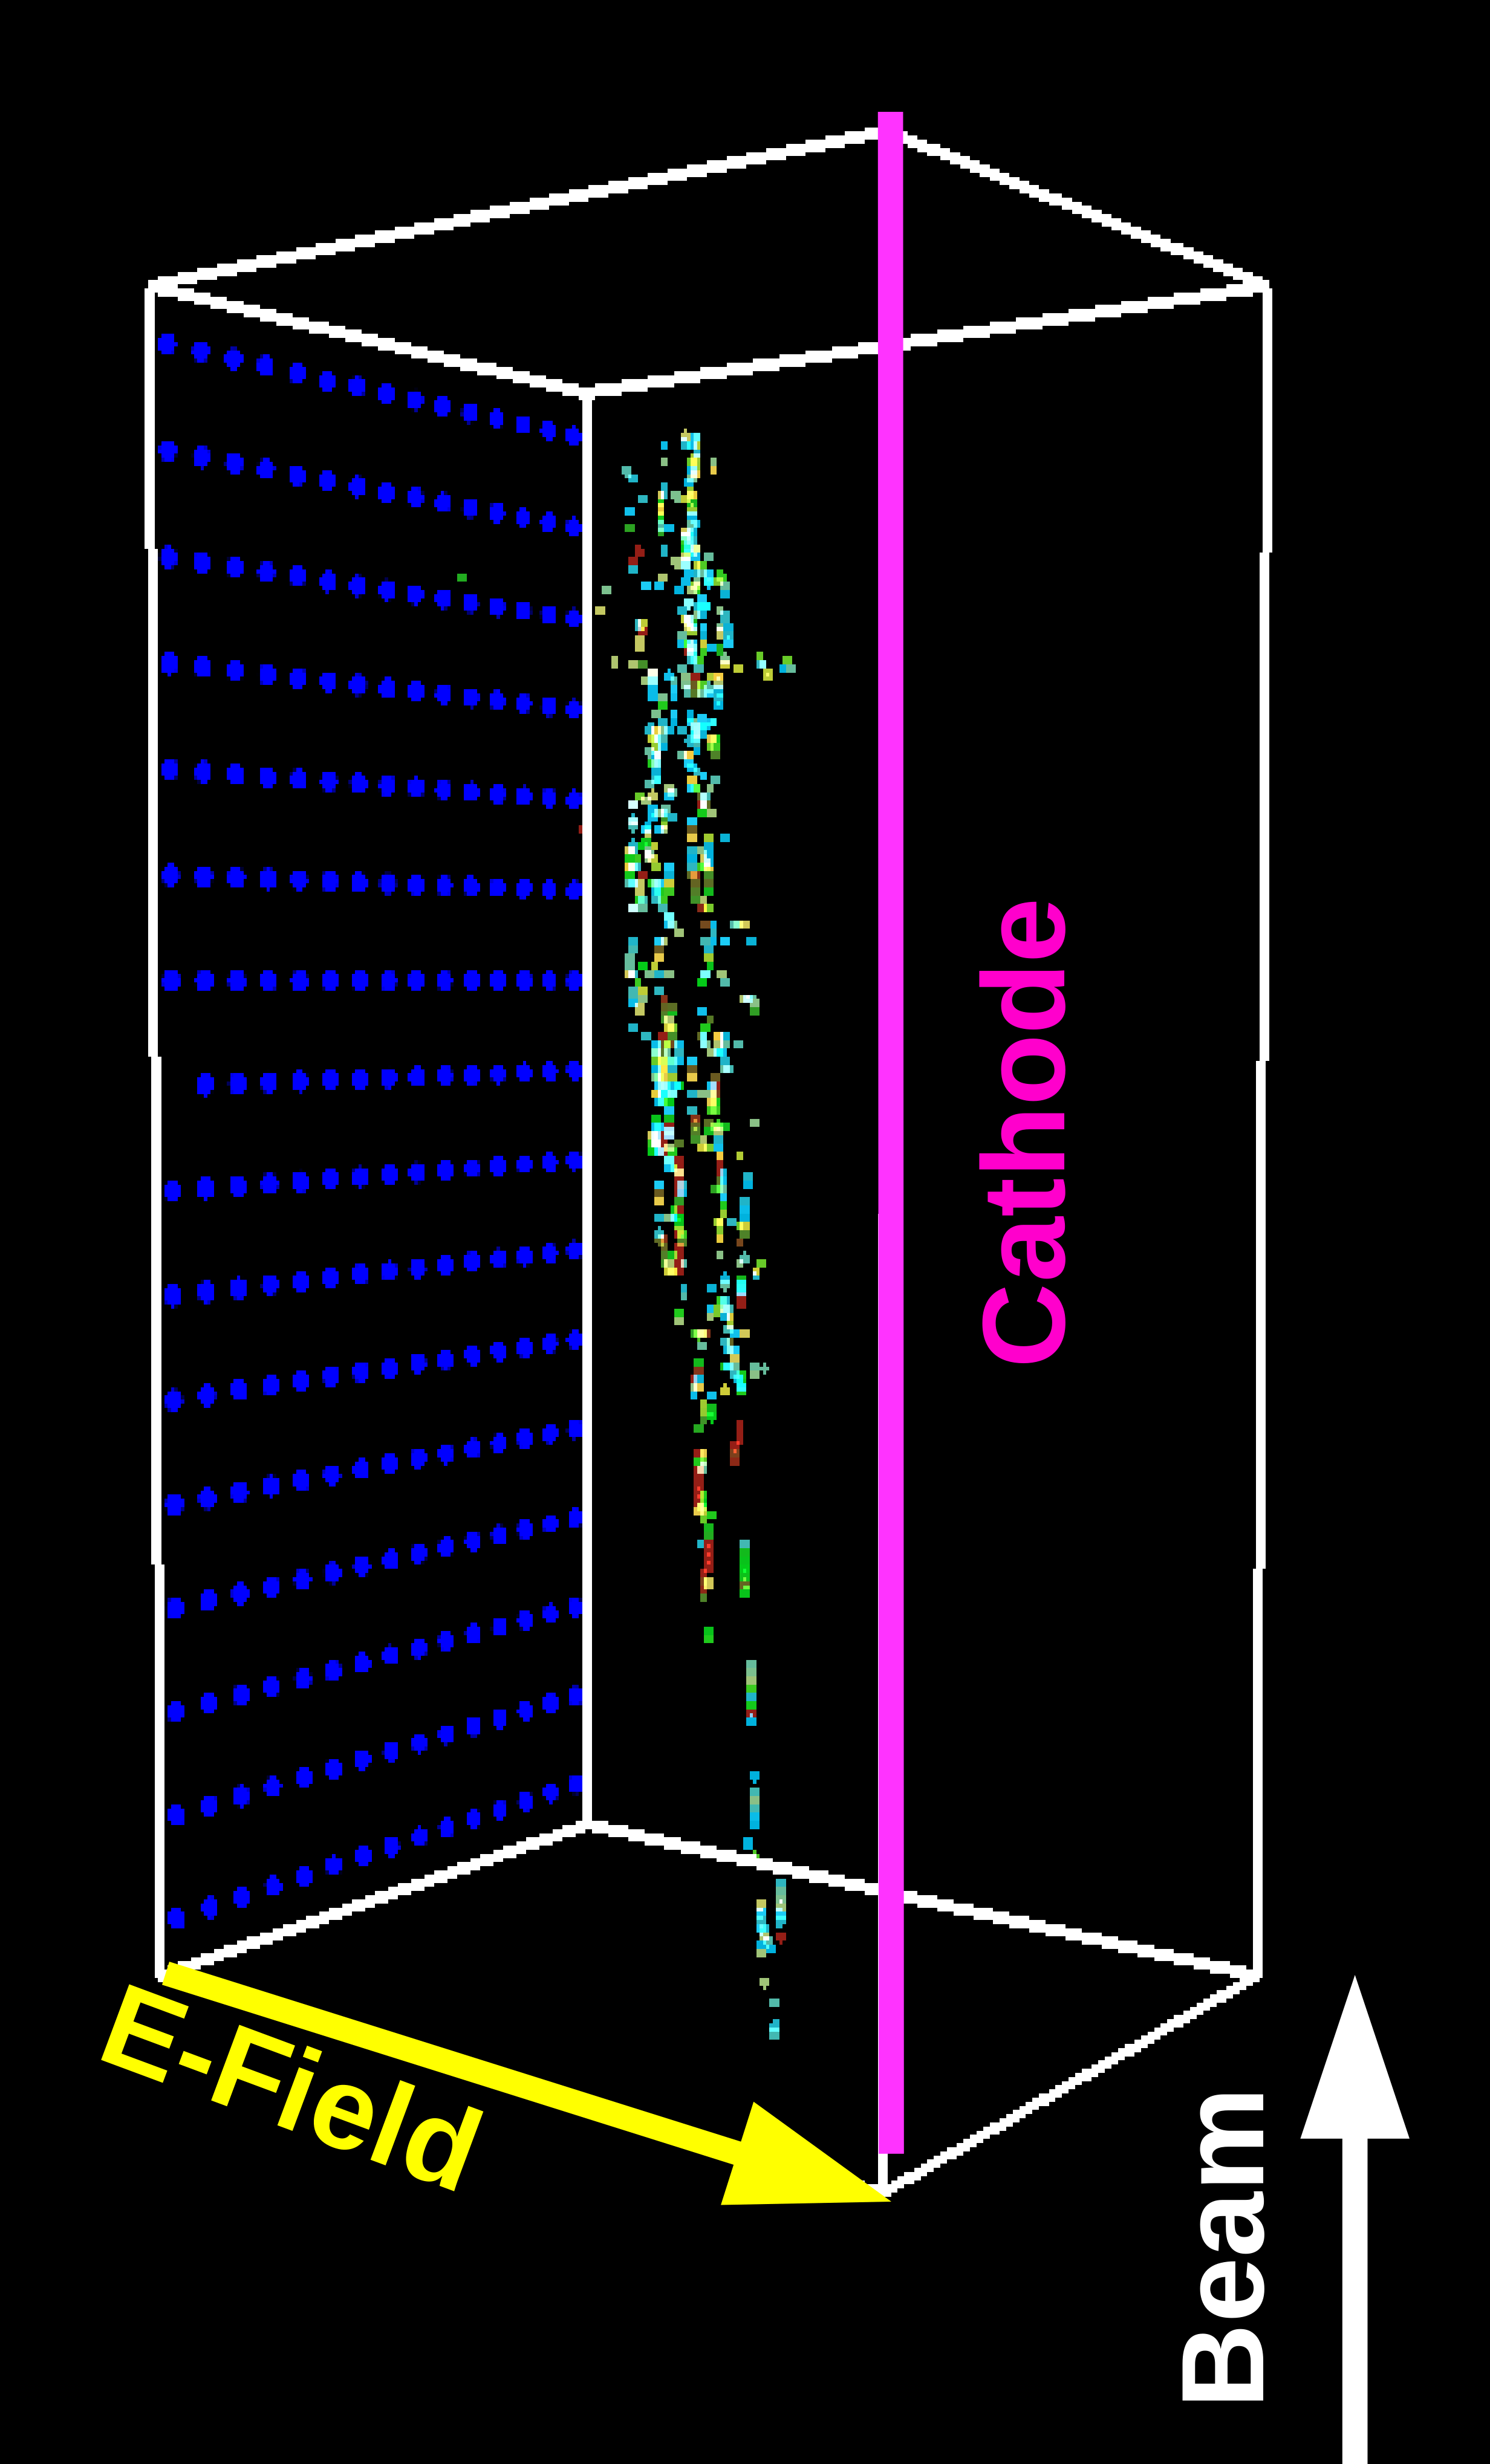
\includegraphics[width=.35\columnwidth]{Figures/pixlar_event_side}
		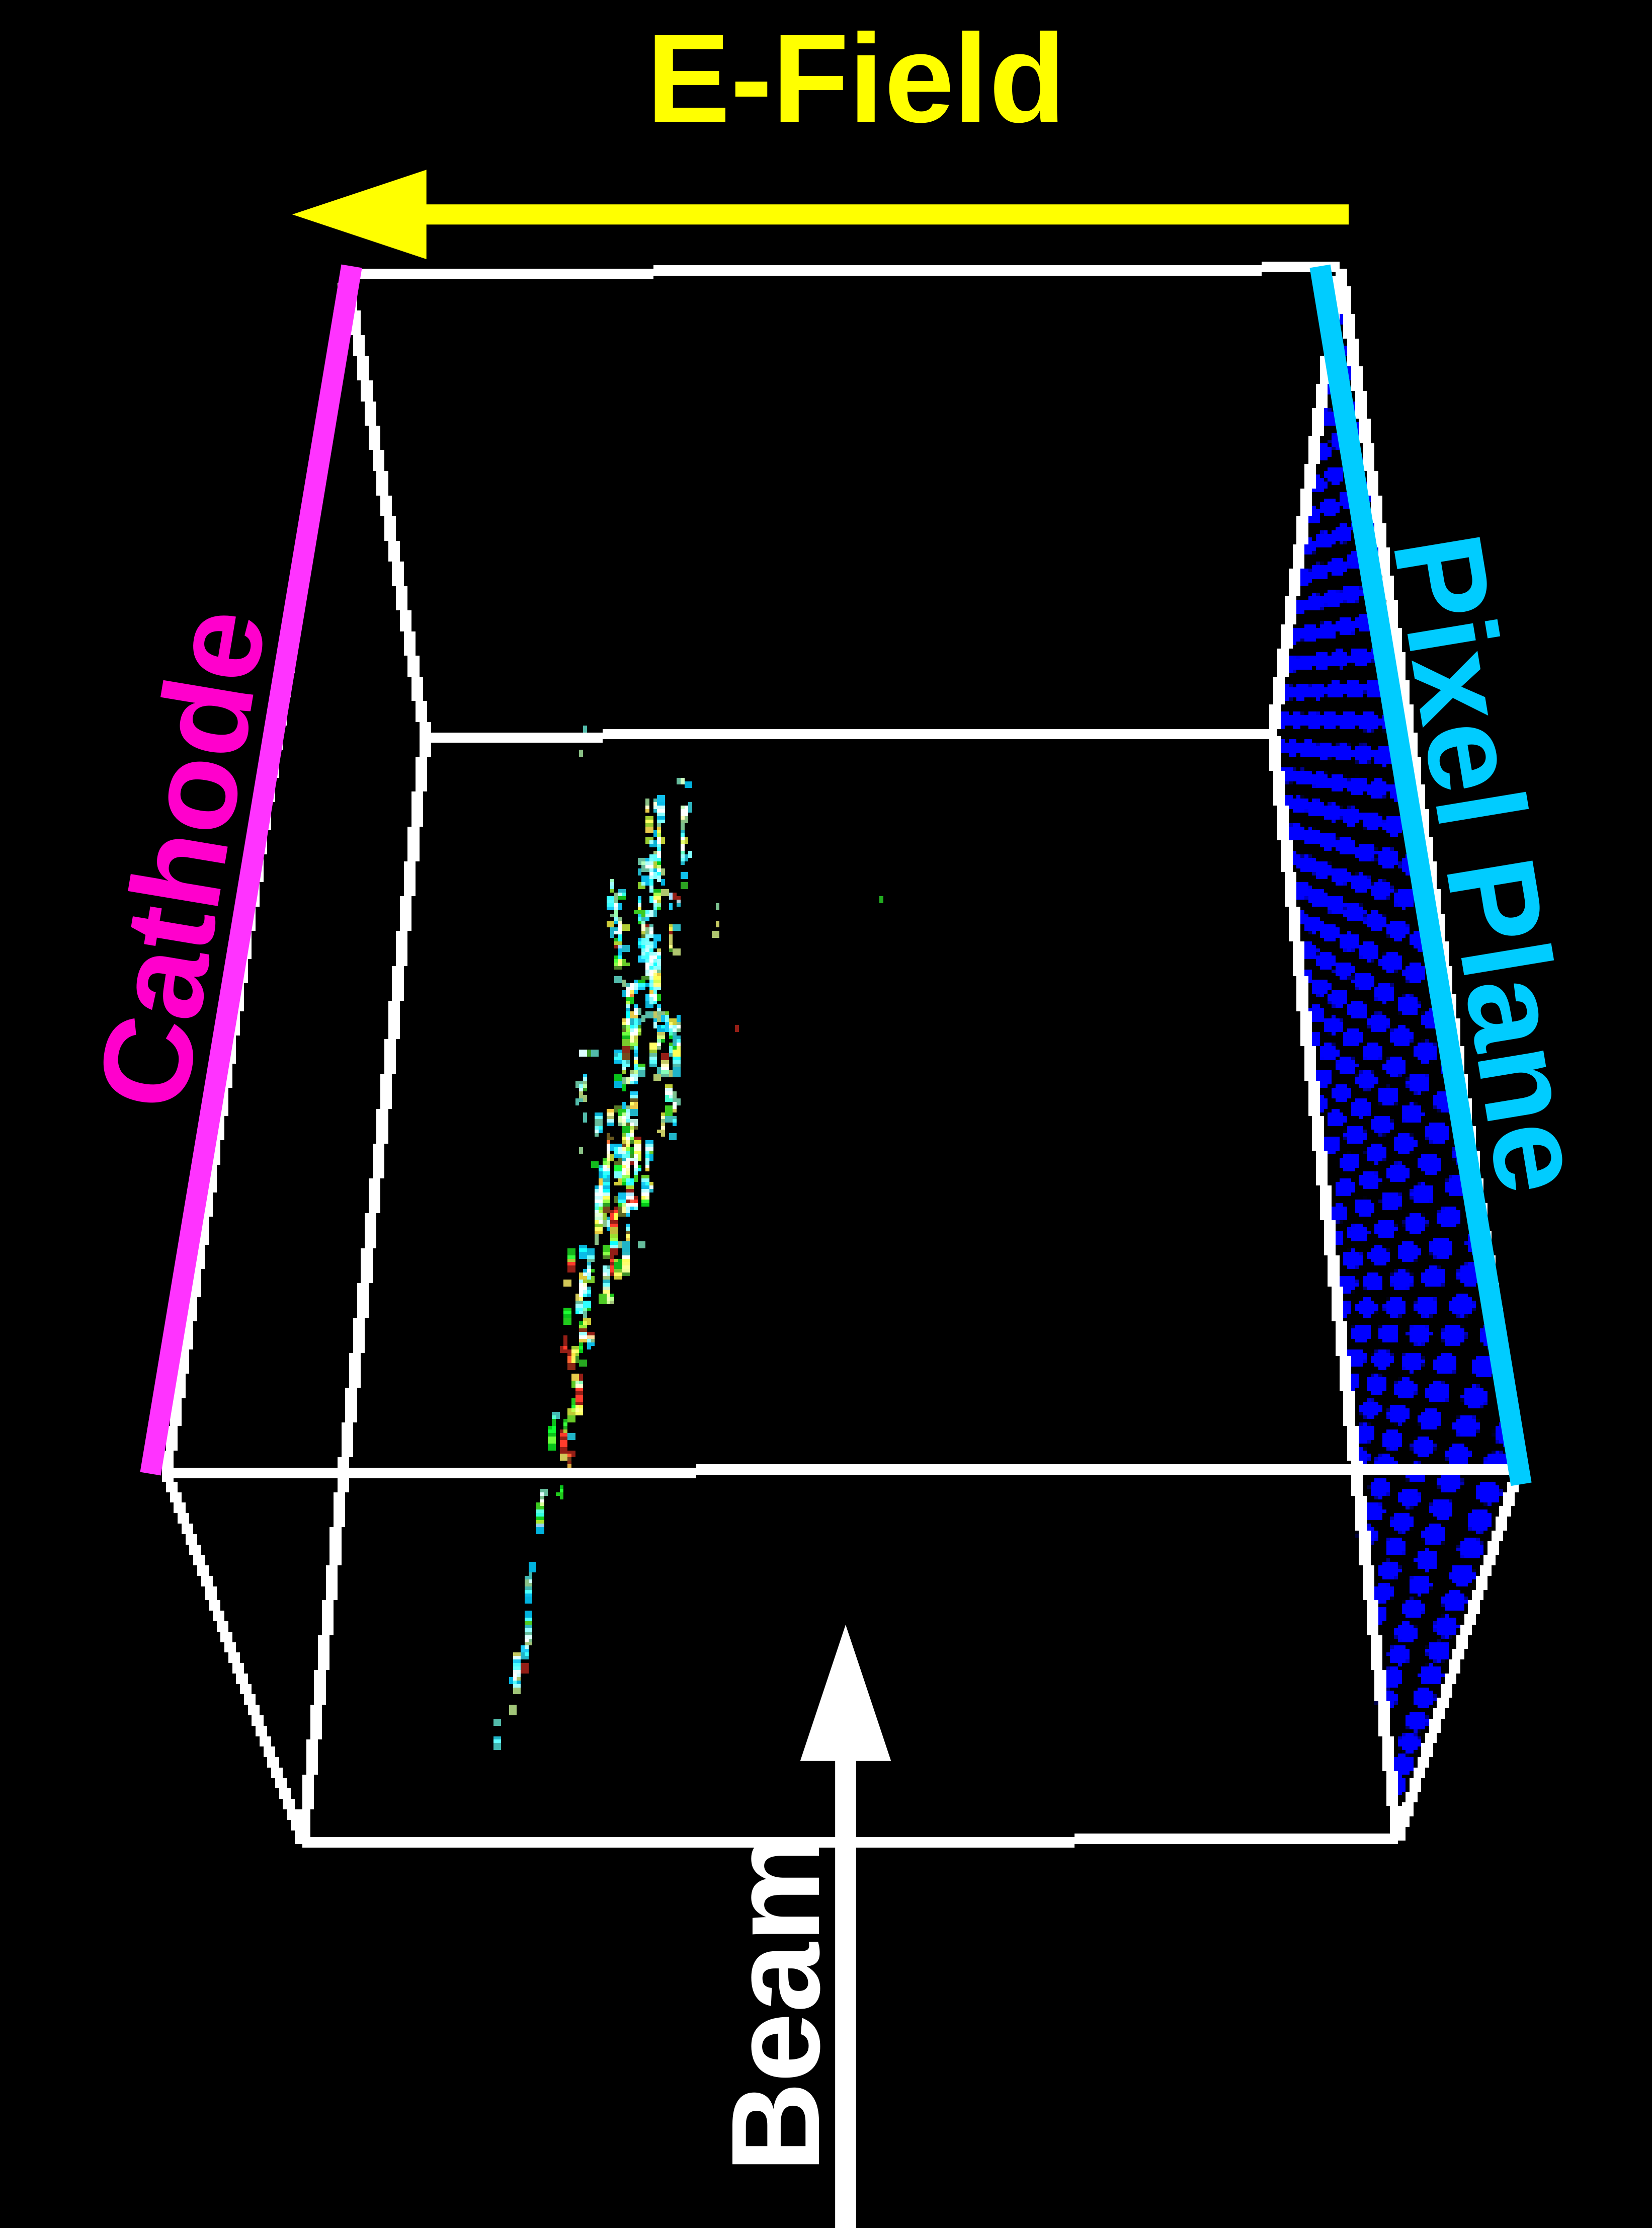
\includegraphics[width=.43\columnwidth]{Figures/pixlar_event_top}
	}
	\caption[PixLAr beam event]{%
		PixLAr beam event.
	}
	\label{fig:pixlar_event}
\end{figure}

Over several weeks beam and cosmic muon data was taken.
At the time of writing no official results were available.
Nevertheless, preliminary analyses indicate a successful scale-up of the pixelated LArTPC concept.
The achieved SNR is comparable to what was reached with the prototype at Bern.
A recorded beam event is shown in Figure~\ref{fig:pixlar_event}.
	
\subsection{Demonstration of Micro-Power 3D Readout}\label{sec:pix}

Providing a unique front-end channel for each pixel is an important next step in the development of true 3D readout for LArTPCs.
With readout densities of $\sim$10$^5$ channels per square meter, this places stringent requirements on electronics design.
In particular, an average power consumption of $\leq$100~$\mu$W per channel is necessary to avoid excessive heating of the cryogenic LArTPC.

Over the past year we have designed and prototyped a micro-power sensor providing true 3D readout at LBNL.
The sensor is based around a custom cryogenic-compatible application-specific integrated circuit (ASIC) called LArPix-v1.
Manufactured in 180~nm bulk CMOS, each ASIC provides 32-channels of charge-sensitive amplification with self-triggered digitization and multiplexed readout at temperatures from 80~K to 300~K.

Using a prototype 128-channel LArPix-based sensor with 3~mm pitch in a 1-liter LArTPC, we have demonstrated low-noise ($<$500 e$^-$ equivalent) low-power ($\sim$60\,$\mu$W/ch) ionization signal detection and readout.
The sensor system was used to successfully measure the three-dimensional ionization distributions of cosmic rays passing through this LArTPC, free from the ambiguities of existing projective techniques, see Figure~\ref{fig:LArPixDemo}.
This prototype sensor demonstrates the feasibility of true 3D pixel readout of LArTPCs.

We are now proceeding to demonstrate the scalability of this technique by instrumenting a sensor with 832 channels.
Assuming the prototype continues to perform well, we plan to produce a second-generation sensor with enhanced features such as a larger dynamic range, improved timing, and more flexible configuration and calibration.


\begin{figure}[htb]
	\centerline{ 
		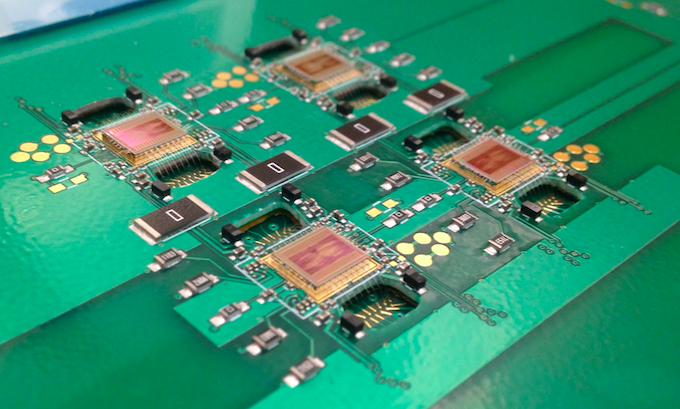
\includegraphics[width=0.5\columnwidth]{Figures/larpix_4chip_top.png}
		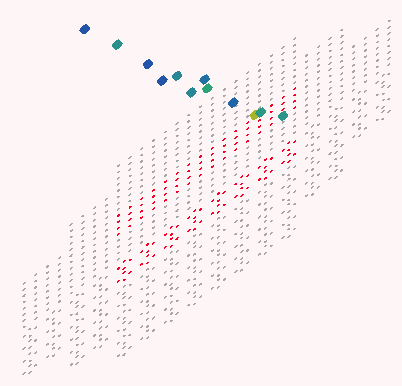
\includegraphics[width=0.35\columnwidth]{Figures/example_track_file3_ev1975.png}
	}
	\caption{ {\em Left:} Four LArPix-v1 application-specific integrated
		circuits (ASICs) used to instrument 128 channels of a prototype 3D
		pixel LArTPC. {\em Right:} The 3D ionization electron distribution
		from a cosmic ray track detected with this sensor (large dots),
		where the color increases from blue to yellow in proportion to
		detected charge.  Only 128 pixels were instrumented for this test
		(red dots).  Instrumentation of the remaining 704 pixels of this
		sensor (grey dots) is in progress.\hfill
		\label{fig:LArPixDemo}}
\end{figure}
	
		
\section{Can ArgonCube Cope in High-Rate Environments?}

The DUNE beam will have an intensity of $\order{\SI{1}{\mega\watt}}$.
Paired with the slow (\si{\milli\second}) nature of LArTPCs this will result in multiple neutrinos interacting inside the detector for each beam spill, so-called event pile-up.
The question is can a ArgonCube disentangle these piled up events?
To assess this one of the most difficult reconstruction tasks---$\pi^0$-induced EM showers---was simulated in an ArC ND geometry.

\subsection{Event Pile-up in the ND}

Extensive detail is provided in this section since this work has faced skepticism on previous presentation. 

\begin{figure}[tbp]
	\centering
	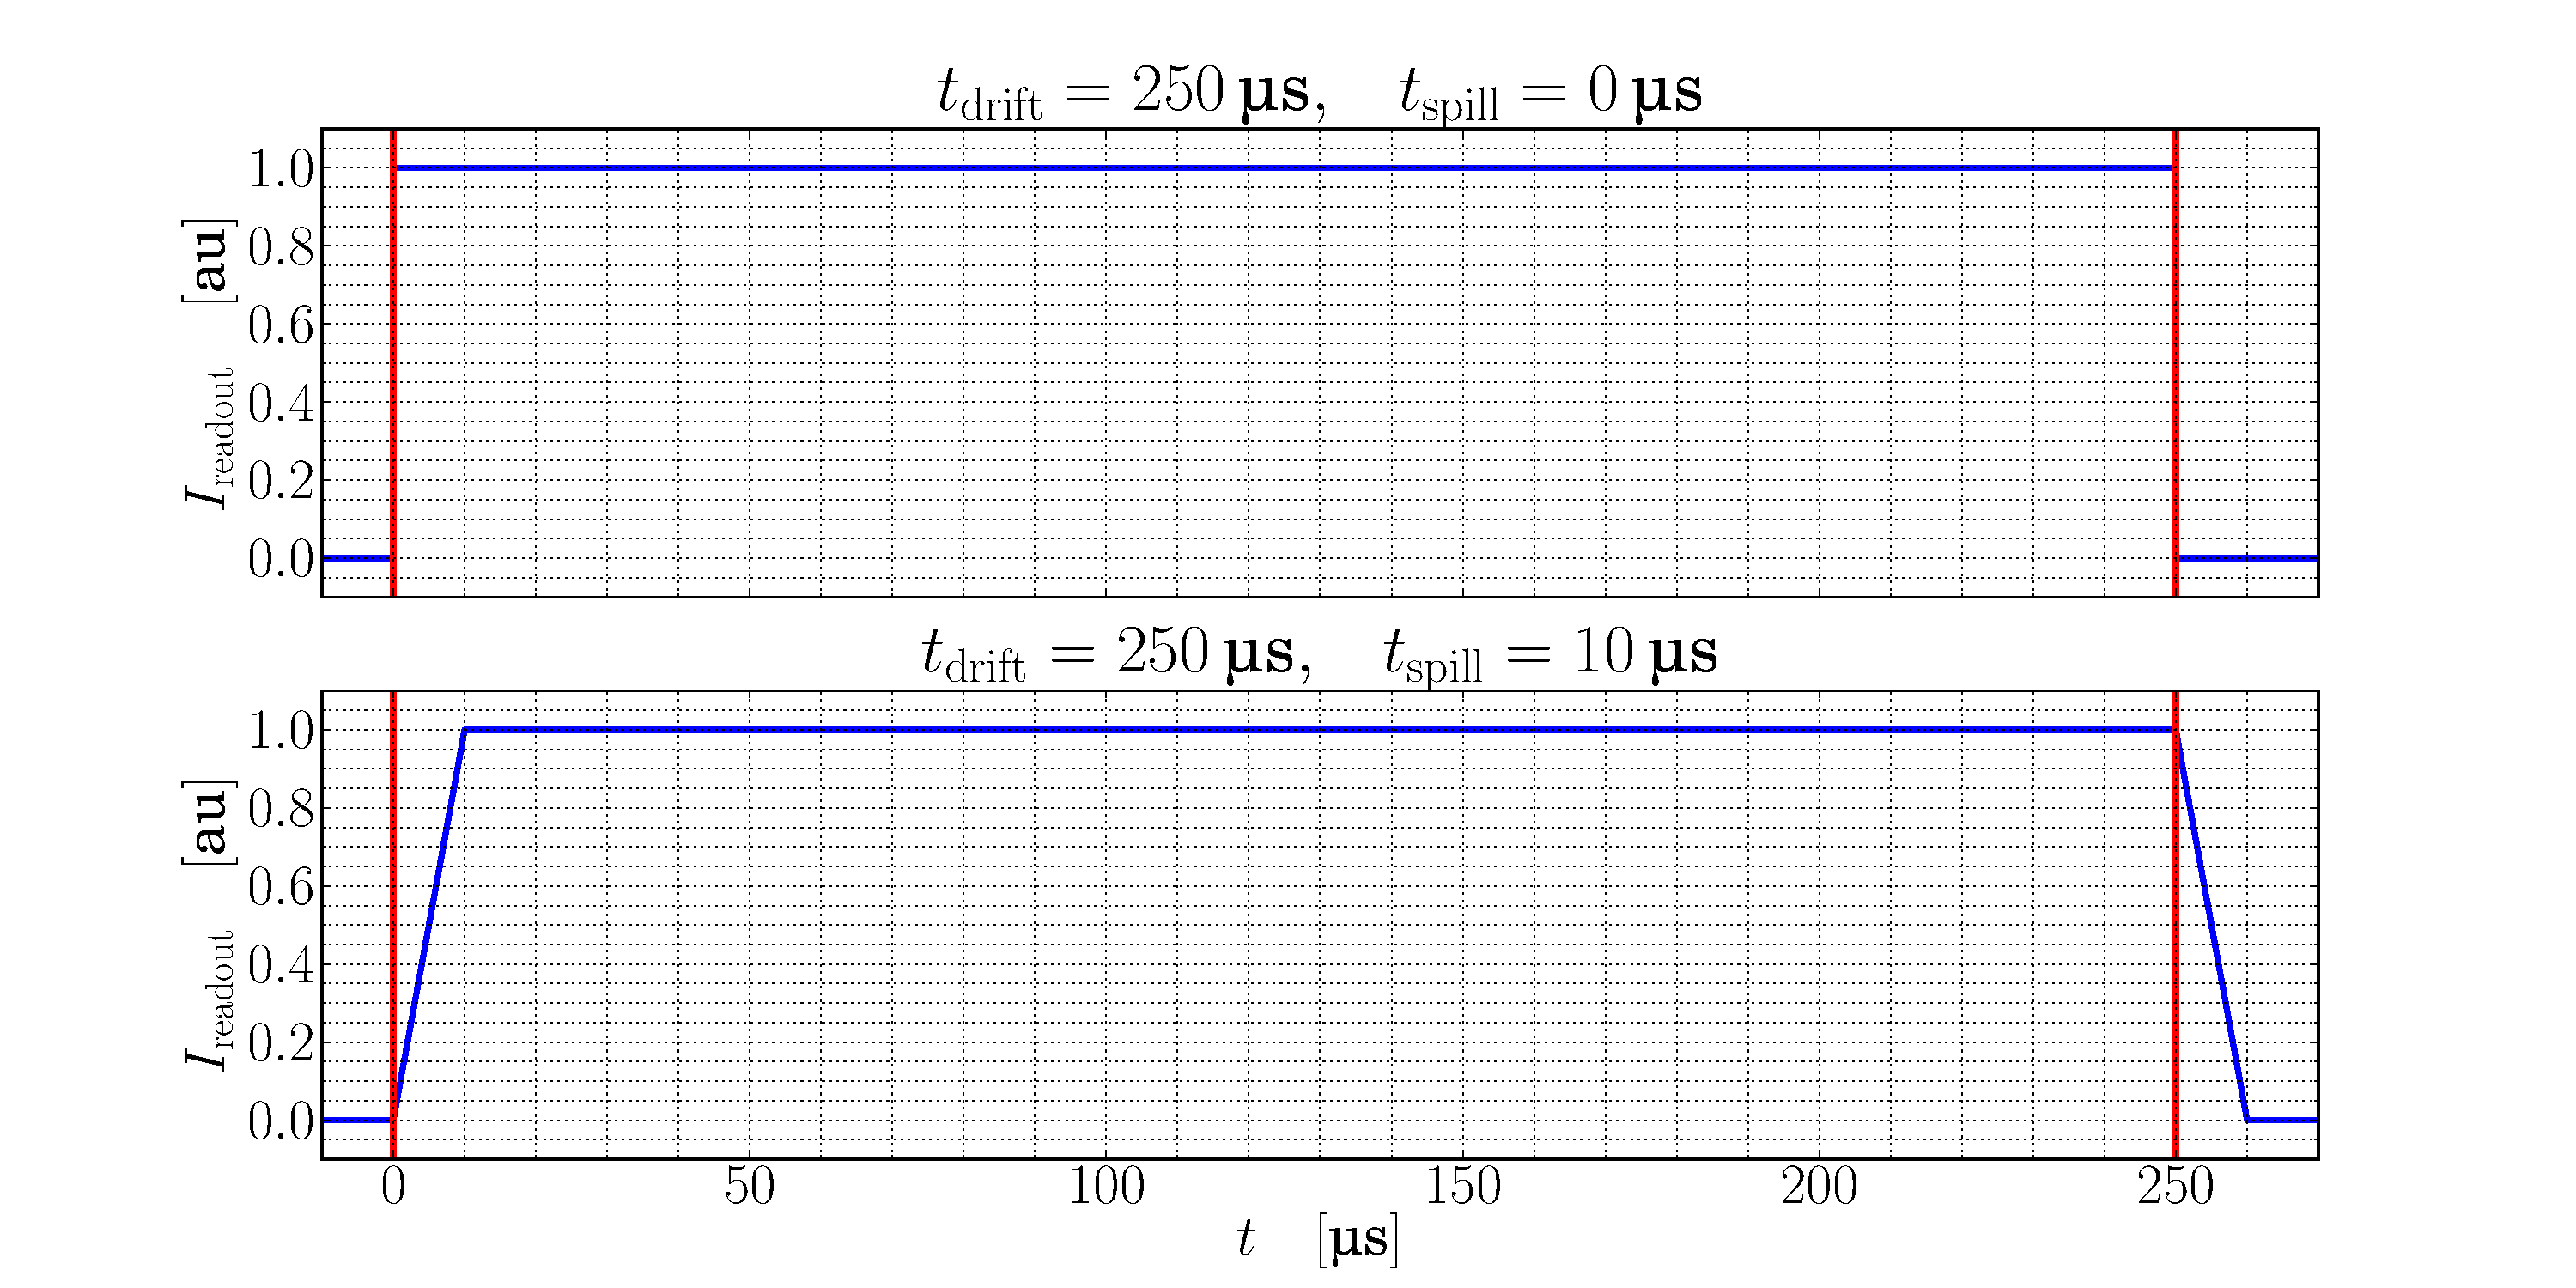
\includegraphics[width=\textwidth]{Figures/charge_flux}
	\caption[Average current collected for one beam spill as a function of time]{%
		Average current collected for one beam spill as a function of time.
		The current is given in arbitrary but equal units for both plots.
		Anode and cathode are represented by the vertical red lines, relative to the trigger timestamp.
		The upper plot assumes the whole charge is deposited instantaneously while for the lower plot the actual spill duration from~\cite{dune2} is used.
	}
	\label{fig:dune-nd_charge-flux}
\end{figure}

LArTPCs are intrinsically slow detectors with a readout time of $\approx \SI{0.5}{\milli\second\per\metre}$ for a \SI{1}{\kilo\volt\per\centi\metre} drift field.
This causes a pile-up of events in the detector; if the readout was infinitely fast, all neutrino interactions could be separated in time.
In reality even the ArC TPCs with a drift length of only \SI{0.5}{\metre}, corresponding to a full readout cycle of \SI{250}{\micro\second}, are significantly slower than the spill duration of \SI{10}{\micro\second} of the DUNE beamline design.
Figure~\ref{fig:dune-nd_charge-flux} visualises this effect.
The charge arriving at the readout is represented as an average current in arbitrary units (same for both plots).
Anode and cathode are represented by the vertical red lines, relative to the trigger timestamp.
The amplitude of the readout current is a direct measure for event pile-up in the corresponding time slice.
For simplicity an infinitely short spill duration was assumed for the pile-up study (top), i.e.\ the whole ionisation charge produced by one beam spill is deposited instantaneously inside the TPC volume.
As the time in between beam spills is $\sim{\SI{1}{\second}}$, all this charge can be read out within one drift time.
In this case the average current (pile-up) seen by the readout is constant over the whole readout cycle.
The realistic case with the spill duration of the DUNE beam is depicted in the bottom plot.
At the beginning of the readout cycle there is no charge deposited yet, the current (pile-up) is zero.
Over the duration of the beam spill ionisation charge accumulates inside the TPC volume while constantly being transported towards the readout by the drift field.
After the beam spill is over the remainder of the initial drift volume (\SI{240}{\micro\second}) contains a uniform charge density.
Due to the finite spill duration there is an additional \SI{10}{\micro\second} (falling) ramp after the first \SI{250}{\micro\second} readout cycle, entering the next readout cycle.
In short, a spill duration shorter than but comparable to the drift time results in the shape of the ionisation current (event pile-up) seen over time to become a trapezoid rather than a square.
The integral, i.e.\ the total ionisation charge (deposited energy), is the same but part of it is shifted from the spill time slice to the beginning of the next readout cycle.
In addition, the peak current (pile-up) stays unchanged as long as the spill duration is shorter than the drift time.
If the spill duration becomes longer than the drift time, the charge is distributed over more than two readout cycles and the peak current (pile-up) begins to decrease.
Therefore, the assumption of an infinitely short spill is a worst-case scenario slightly improved by the real, finite spill duration.
However, for \SI{96}{\percent} of the drift time (\SI{240}{\micro\second}) pile-up is unchanged.


\subsection{Feasibility Study of a Pixelated LArTPC in the Near Detector}

\begin{table}[tbp]
	\centering
	\caption{Parameters of the $\pi^0$ pile-up simulation.}
	\label{tab:dune-nd_pile-up-params}
	\begin{tabu} to \textwidth {lSs}
		\toprule
		Parameter &						{Value} &				{Unit} \\
		\midrule
		X-axis orientation &			{Drift} &				\\
		Y-axis orientation &			{Vertical} &			\\
		Z-axis orientation &			{Beam} &				\\
		Resolution X &					3 &						\milli\metre \\
		Resolution Y &					3 &						\milli\metre \\
		Resolution Z &					3 &						\milli\metre \\
		Target volume X &				\numrange{-100}{500} &	\centi\metre \\
		Active volume X &				\numrange{0}{400} &		\centi\metre \\
		Fiducial volume X &				\numrange{30}{370} &	\centi\metre \\
		Target volume Y &				\numrange{-100}{350} &	\centi\metre \\
		Active volume Y &				\numrange{0}{250} &		\centi\metre \\
		Fiducial volume Y &				\numrange{30}{220} &	\centi\metre \\
		Target volume Z &				\numrange{-400}{500} &	\centi\metre \\
		Active volume Z &				\numrange{0}{500} &		\centi\metre \\
		Fiducial volume Z &				\numrange{30}{470} &	\centi\metre \\
		Detection threshold &			0.1 &					\mega\electronvolt \\
		Cone extent &					10 &				 	\radlen \\
		Cone aperture (full angle) &	30 &					\degree \\
		Cylinder diameter &				5 &						\centi\metre \\
		Beam intensity &				2.14 &					\mega\watt \\
		Proton energy &					80 &					\giga\electronvolt \\
		Events per beam spill &			0.21 &					evt\per\tonne_{\ce{Ar}}\\
		\bottomrule
	\end{tabu}
\end{table}


Reconstruction complexity paired with potential impact on physics measurements make photons produced by $\pi^0$ decays a good sample to study the robustness to pile-up of a pixelated LArTPC in the DUNE ND environment.
Energy misidentifications lead to a misreconstructed neutrino energy.
The resulting discrepancy to the true neutrino energy has the potential to skew the measured energy spectrum and thus impact the oscillation measurements.
A significant amount of $\pi^0$ are produced in various RES and COH neutrino interaction modes~\cite{dune2}.
They decay according to

\begin{equation*}
	\pi^0\rightarrow\gamma\gamma,
\end{equation*}

with a branching ratio of \SI{98.8}{\percent}~\cite{pdg}.
The photons subsequently produce EM showers in LAr.
At the energies of the DUNE beam, most showers do not deposit a homogeneous cone of charge but rather a lot of individually resolvable $e^\pm$ tracks.
More importantly, there are often significant gaps in between these charge clusters.
A main challenge of shower reconstruction is to associate these well separated charge blobs to the correct event.

\begin{figure}[tbp]
	\centering
	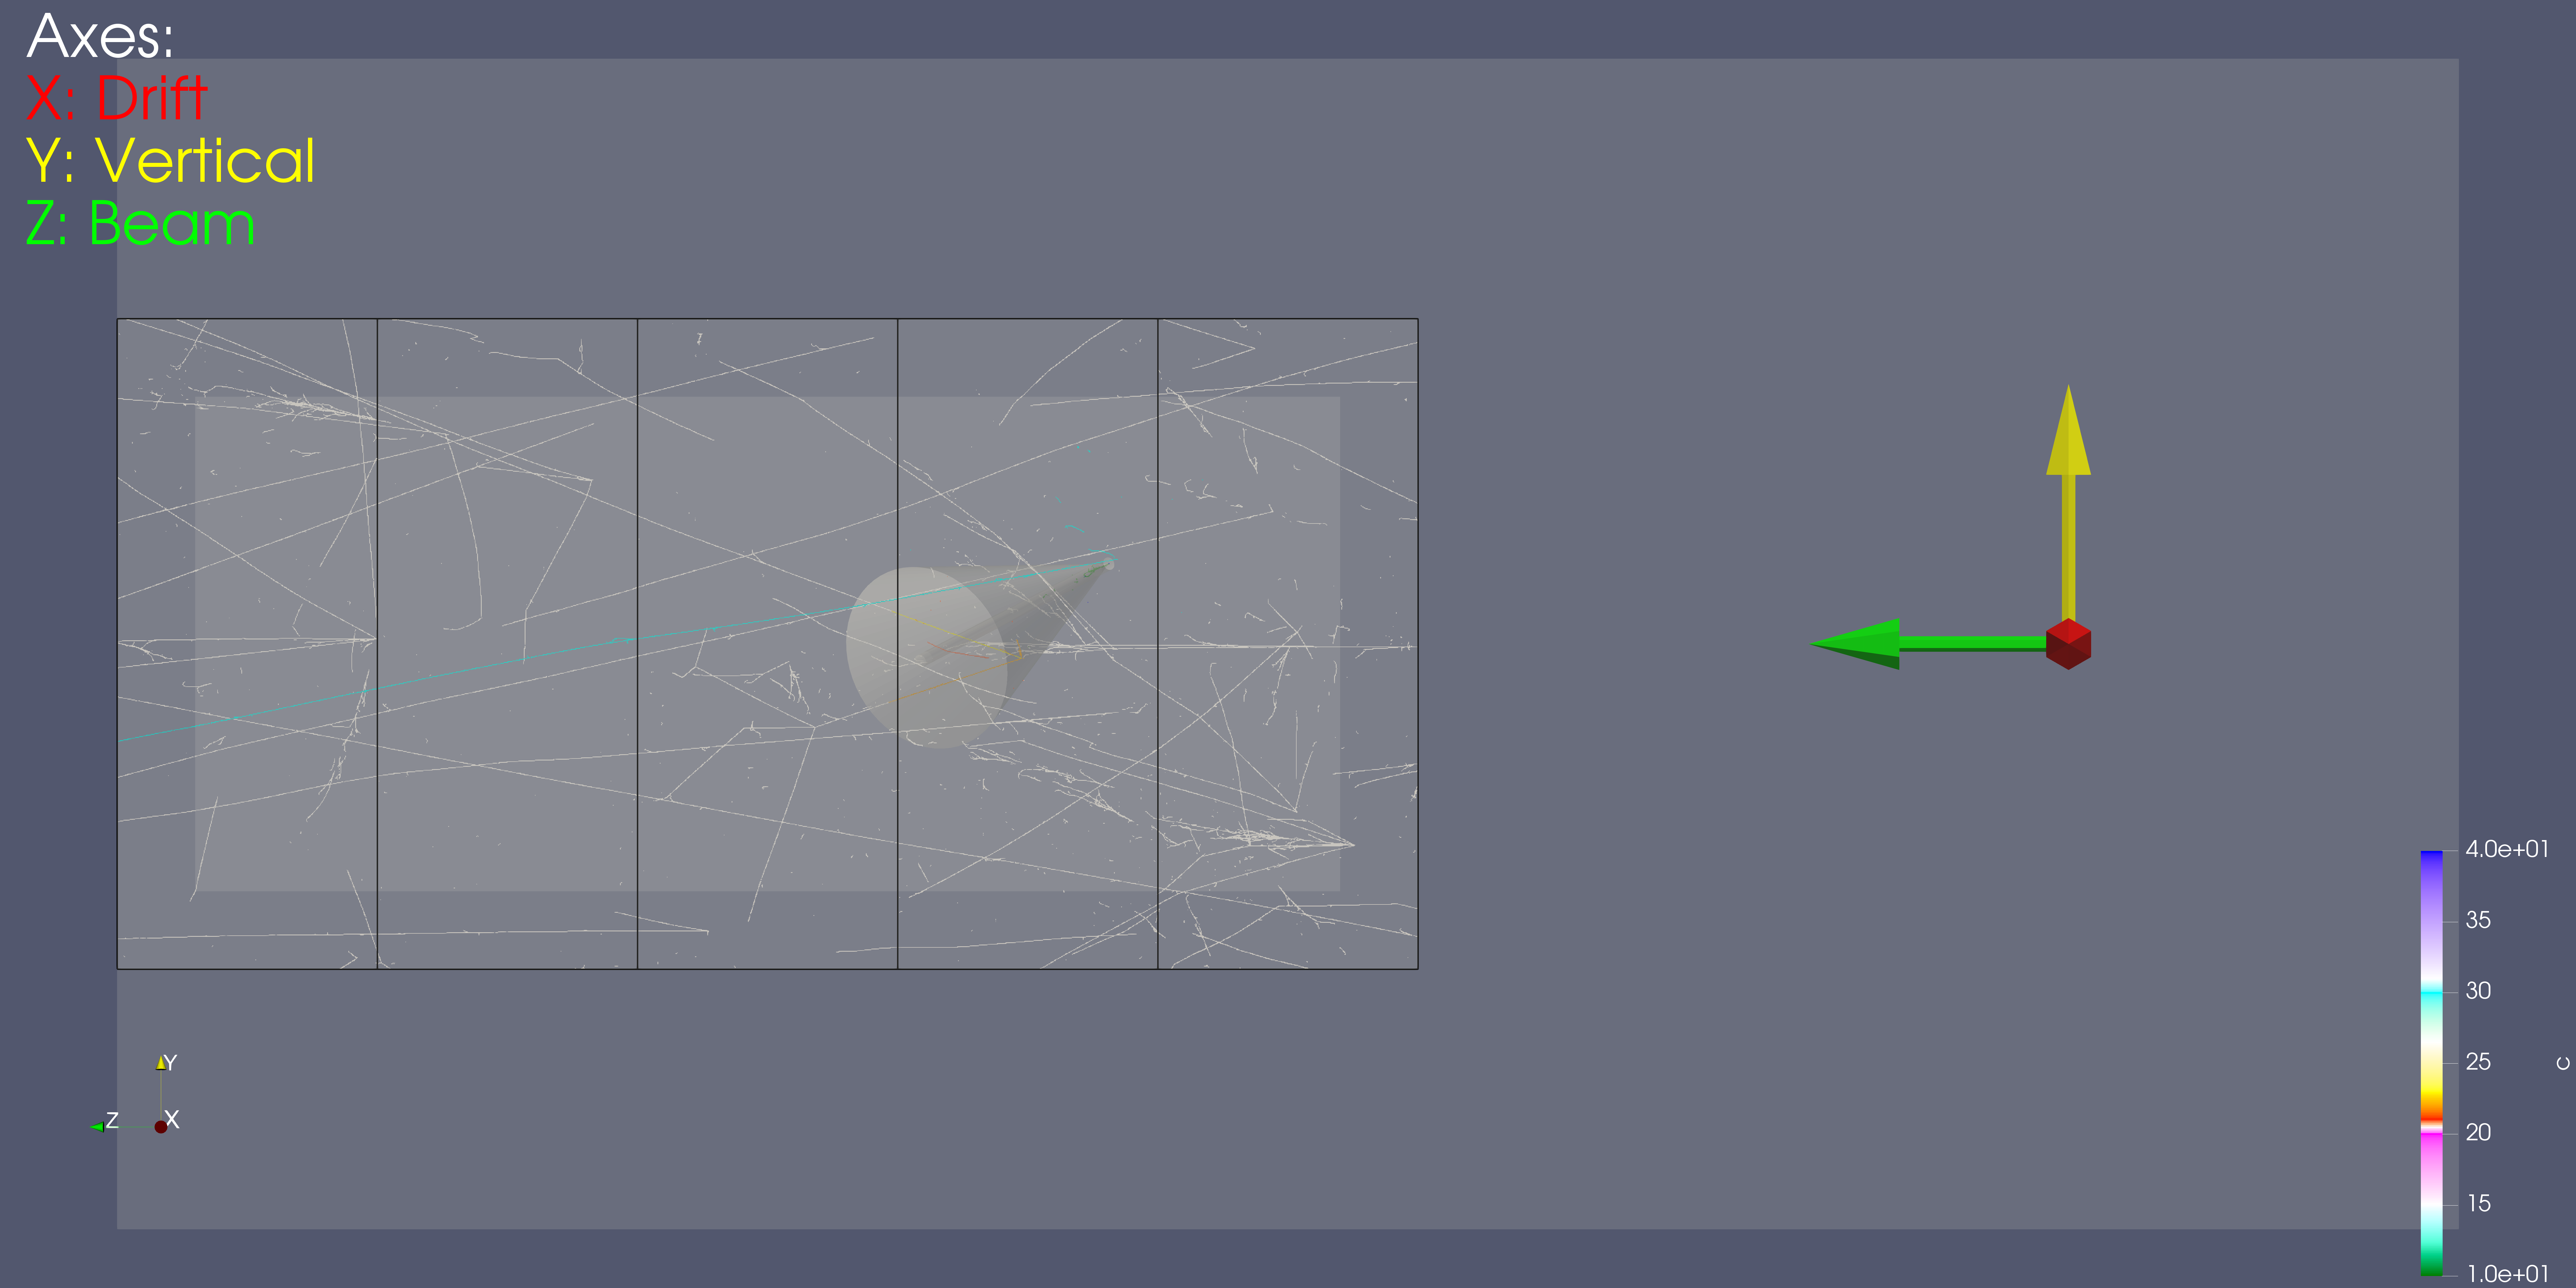
\includegraphics[width=\textwidth]{Figures/uid0_spill6_event461_gamma19_x}
	\caption[Pile-up study example event]{%
		Event display showing a simple $\pi^0$-induced EM shower reconstruction algorithm based on a cone-cylinder union, simulated for the ArC ND component.
		Visible are the three different volumes used for the simulation.
		The outermost volume is used to simulate rock events.
		The active detector volume is represented by the intermediate volume, divided into modules by vertical black lines.
		In order to reduce the number of EM showers not depositing any energy inside the detector a fiducial volume (the innermost) is defined, and photons are required to be produced therein.
		Depicted is a side view of the detector, looking in drift direction.
		The detailed orientation is indicated by the coloured arrows.
	}
	\label{fig:dune-nd_example-display}
\end{figure}

To simulate the expected neutrino interactions in the ND the LBNL Argon Box simulation tool was used.
For this study \num{6.6e6} neutrino events, produced with the GENIE. neutrino event generator, were used.
Secondary particle transport and interaction in Argon Box is performed by Geant4.
Finally, the energy deposition in LAr is voxelised and stored together with all the necessary ancillary information about the depositing particle.

\begin{figure}[tbp]
	\centering
	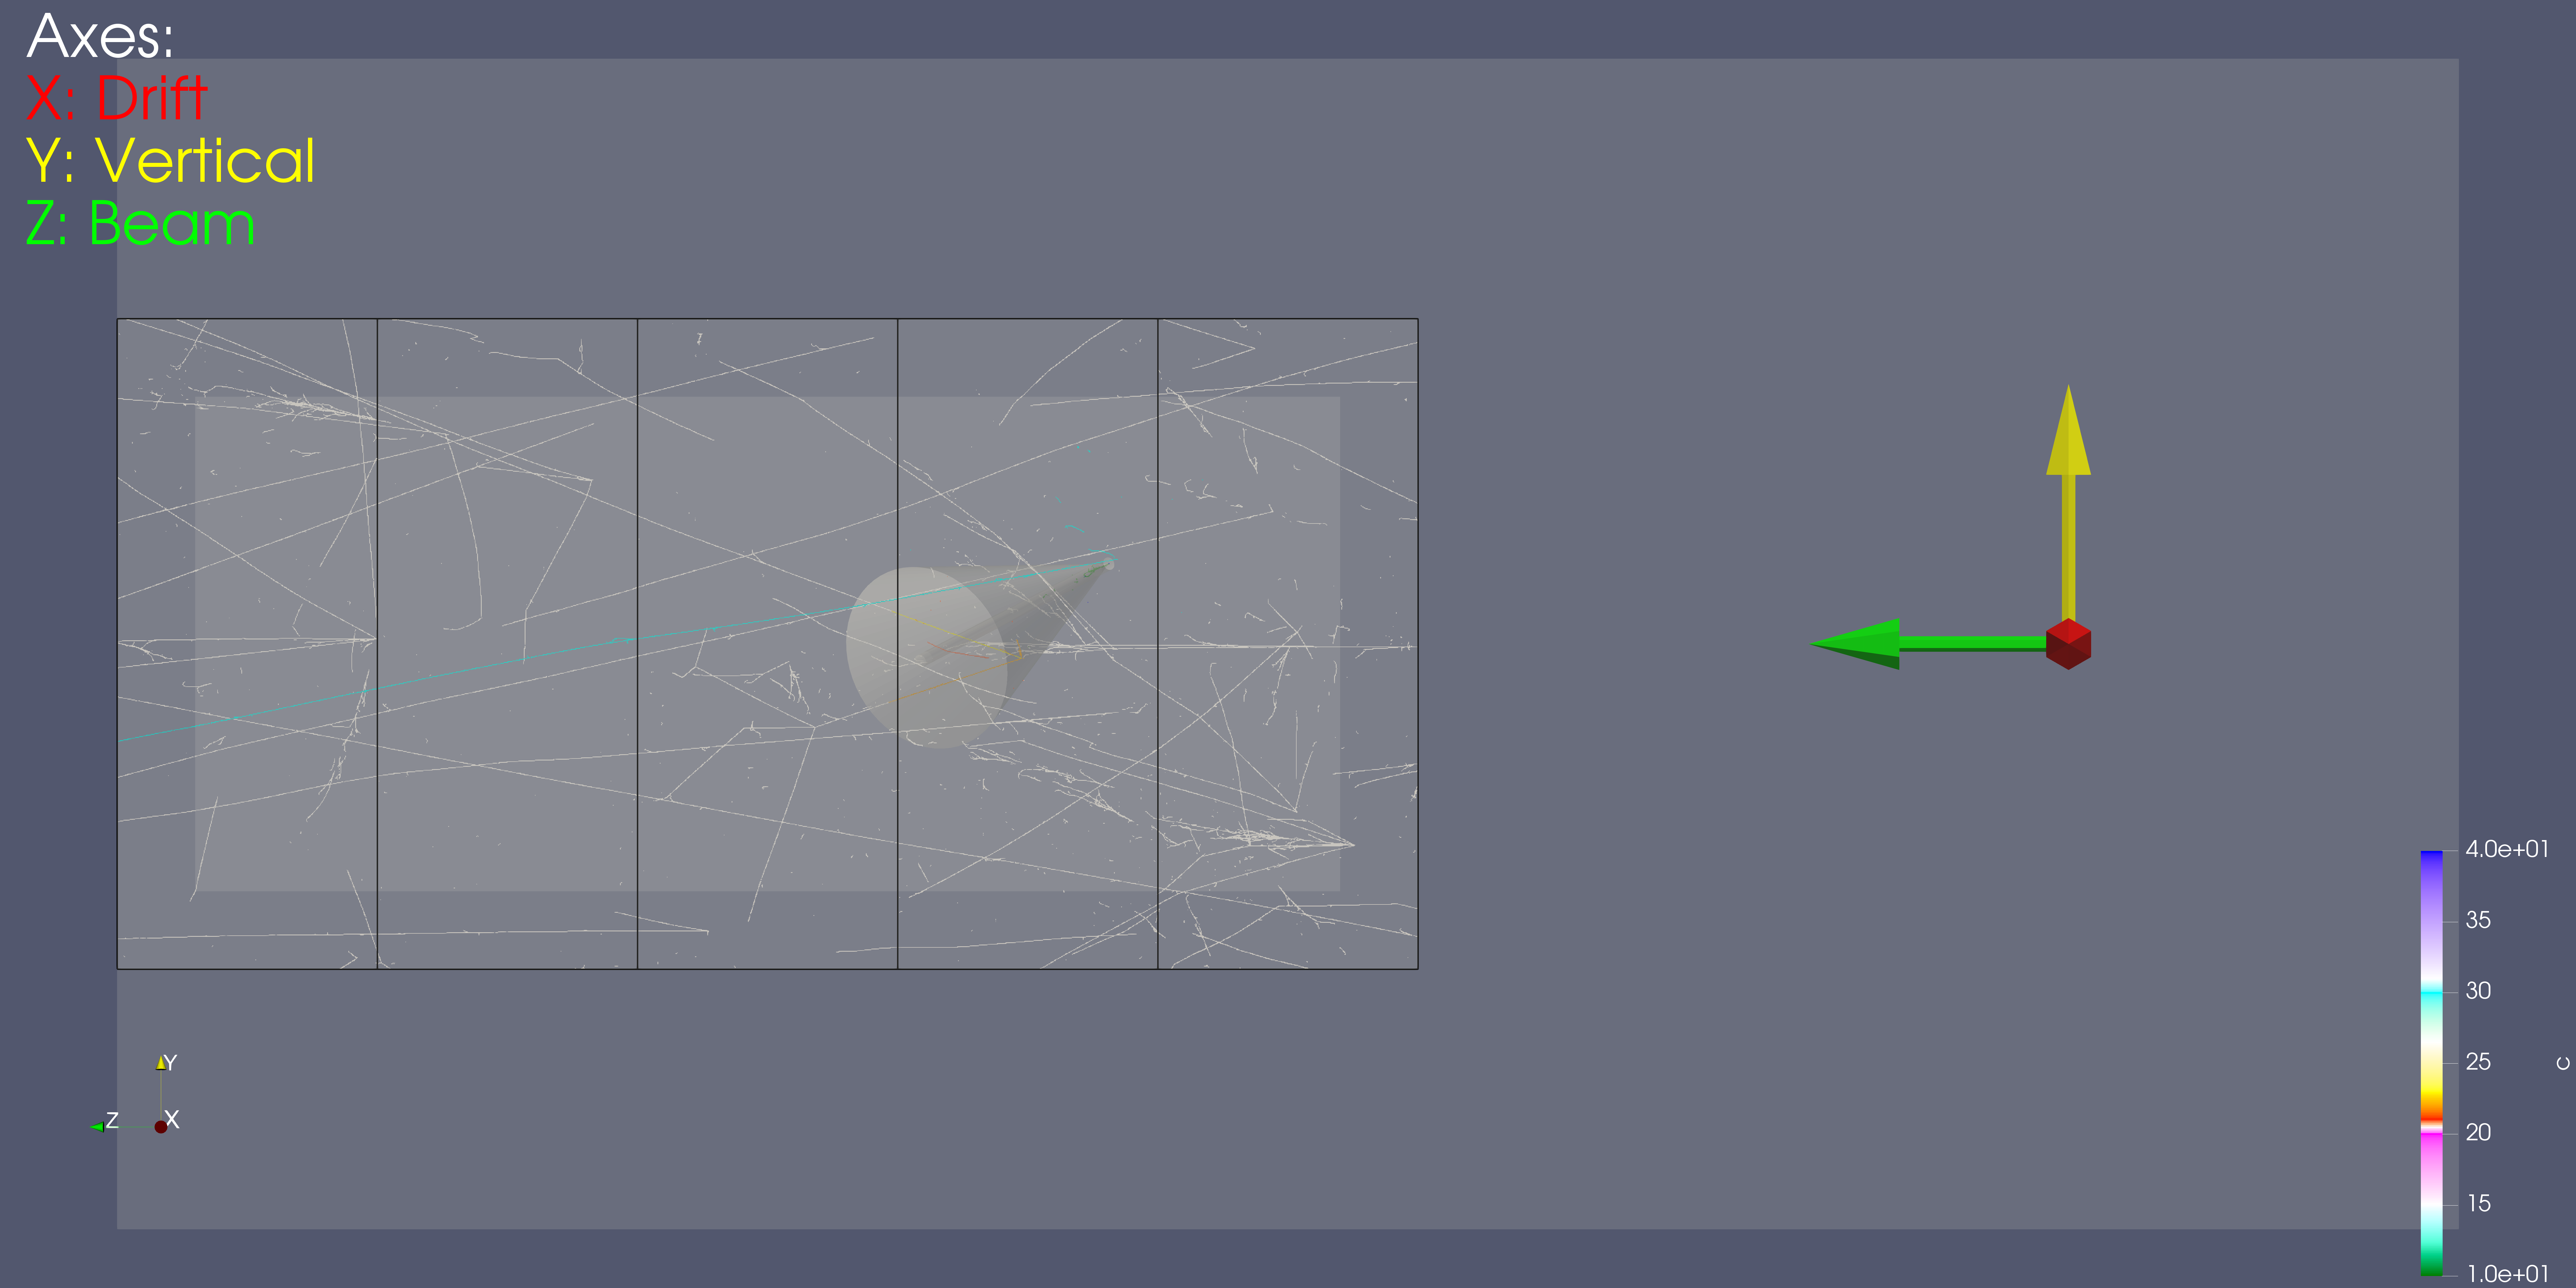
\includegraphics[viewport=2900 1800 4000 2600, clip, width=\textwidth]{Figures/uid0_spill6_event461_gamma19_x}
	\caption[Pile-up study example event close-up]{%
		Close-up view of the pile-up event shown in Figure~\ref{fig:dune-nd_example-display}.
		The acceptance volume is defined by the union of cone and cylinder.
		Charge depositions are depicted by white and coloured voxels whose size represents the applied resolution of \SI{3}{\milli\metre} in all directions.
		Colour indicates type and acceptance of energy deposition.
		White: Different neutrino event, outside acceptance volume.
		Cyan: Correct neutrino event but not part of considered EM shower, outside acceptance volume.
		Dark blue: Correct neutrino event and EM shower, outside acceptance volume (missed energy).
		Green: Correct neutrino event and EM shower, inside acceptance volume.
		Magenta: Correct neutrino event but not part of considered EM shower, inside acceptance volume (not present in this example).
		Yellow (muons), Red ($\gamma$, $n$, and descendants), Orange (neither): Different neutrino event, inside acceptance volume (misidentified energy).
	}
	\label{fig:dune-nd_example-display-zoom}
\end{figure}

To investigate the effects of pile-up on energy reconstruction a working reconstruction algorithm is necessary.
However, at the time of writing existing reconstruction tools were only available for LArTPCs read out by wire planes.
Therefore, a simple algorithm for true 3D space points was implemented, under the assumption that a positive outcome of such a pile-up study would imply an even better performance of a more sophisticated reconstruction.
This algorithm is explained in the following, its parameters are listed in Table~\ref{tab:dune-nd_pile-up-params}, an example of a simulated event is shown in Figures~\ref{fig:dune-nd_example-display} and~\ref{fig:dune-nd_example-display-zoom}.

\begin{figure}[tbp]
	\centering
	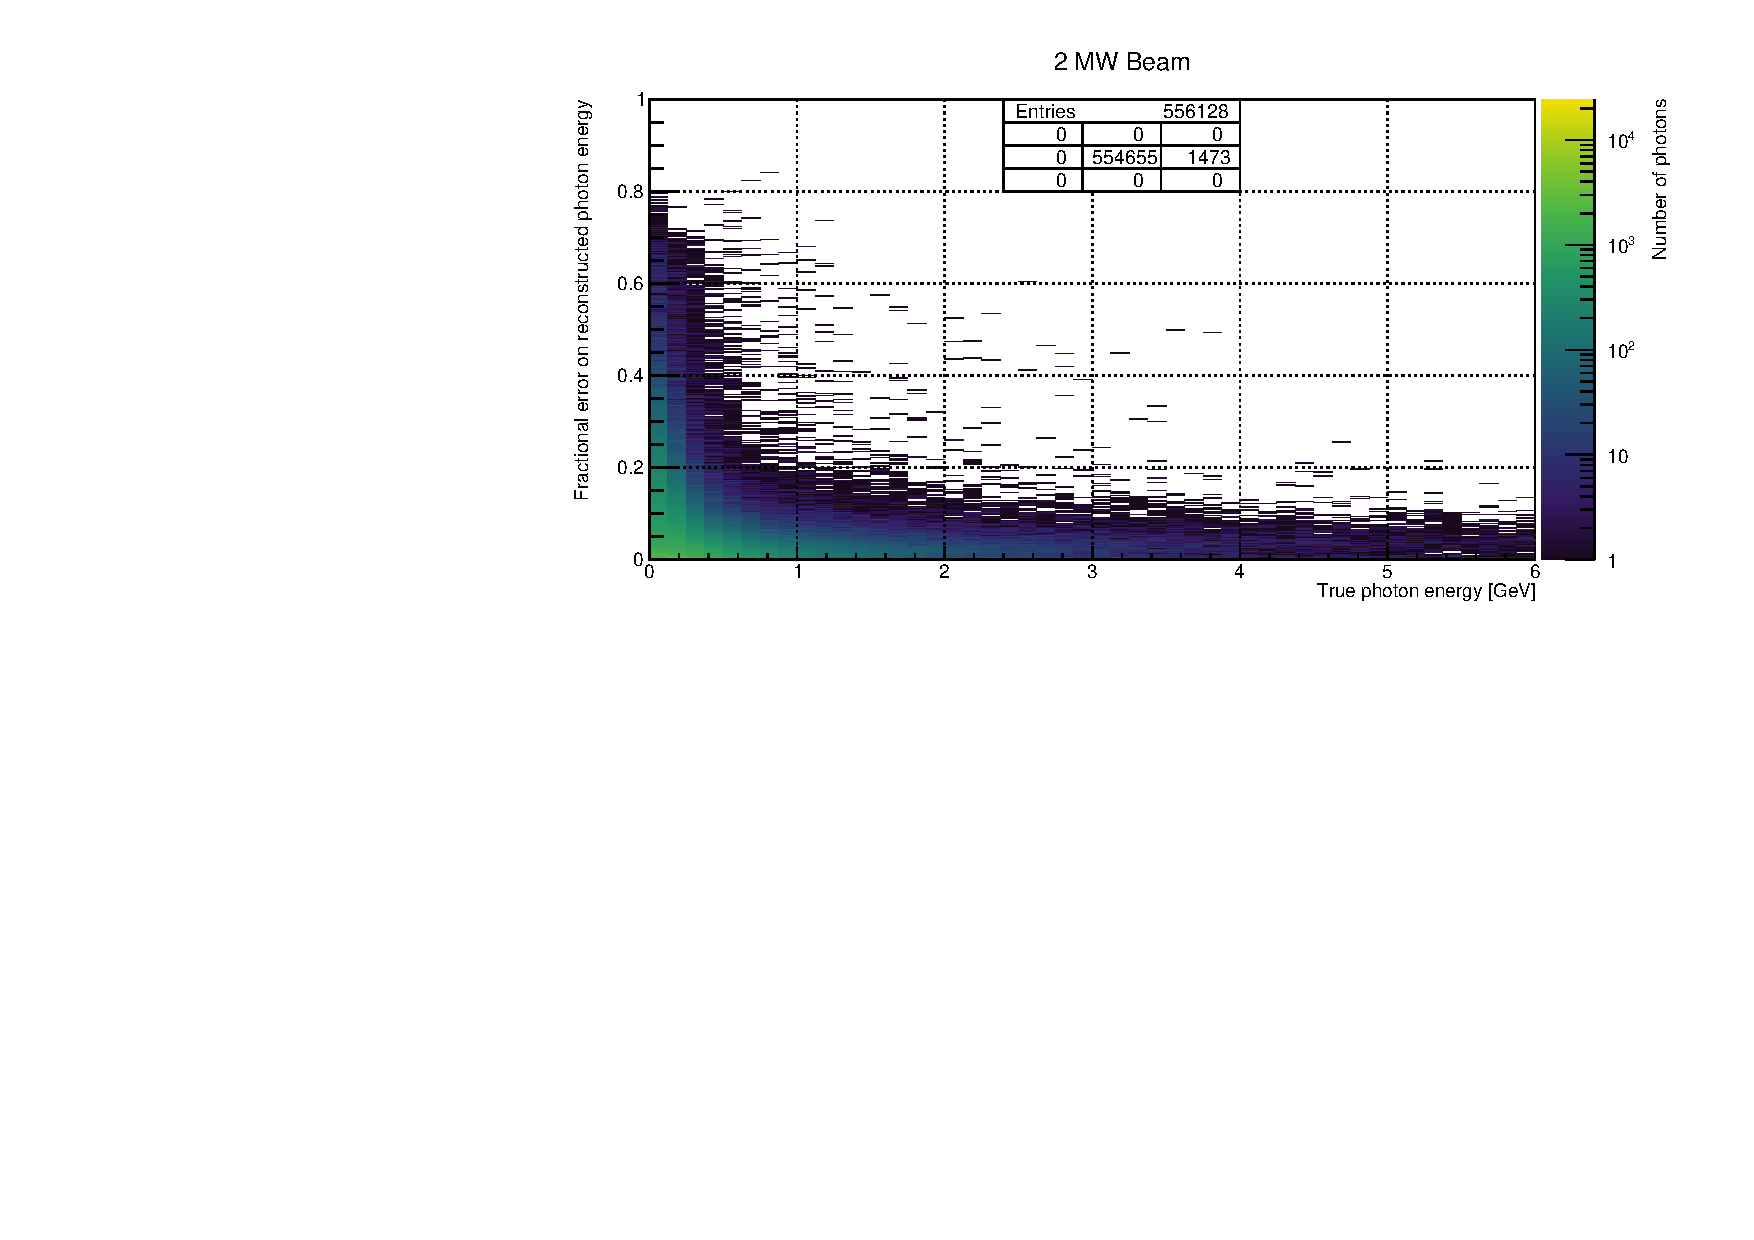
\includegraphics[width=\textwidth]{Figures/2MW/rel_2d_missed}
	\caption[Pile-up study missed fractional vs.\ true photon energy, \SI{2}{\mega\watt} beam]{%
		Missed energy fraction versus true photon energy for a simple $\pi^0$-induced EM shower reconstruction algorithm based on a cone-cylinder union.
		All energy deposited outside of the cone-cylinder union is counted as missed.
		\SI{2}{\mega\watt} beam of \SI{80}{\giga\electronvolt} protons.
		Entries: Central cell shows plotted entries, other cells show overflow entries in direction w.r.t.\ central cell.
	}
	\label{fig:dune-nd_2MW_rel-2d-missed}
\end{figure}

The basic underlying assumption is that a pixel readout with LArPix will yield unambiguous 3D space points of charge deposition with a given resolution, depending on the geometry of the pixel plane, time resolution of the readout electronics, and charge transport effects.
In Section~\ref{sec:pix} LArPix has been shown to be feasible.
The spatial resolution of the pixel readout is assumed to be \SI{3}{\milli\metre} in both directions, in line with what has already been achieved.
A conservative value of \SI{3}{\milli\meter} was chosen in drift direction.
This has several advantages.
Choosing the same resolution as the pixel pitch makes the simulation independent of TPC orientation.
MicroBooNE has achieved a resolution in drift direction $< \SI{3}{\milli\metre}$~\cite{uboner}, making it safe to assume LArPix will enable a similar performance with ArC.
A conservative value also accounts for charge diffusion.

\begin{figure}[tbp]
	\centering
	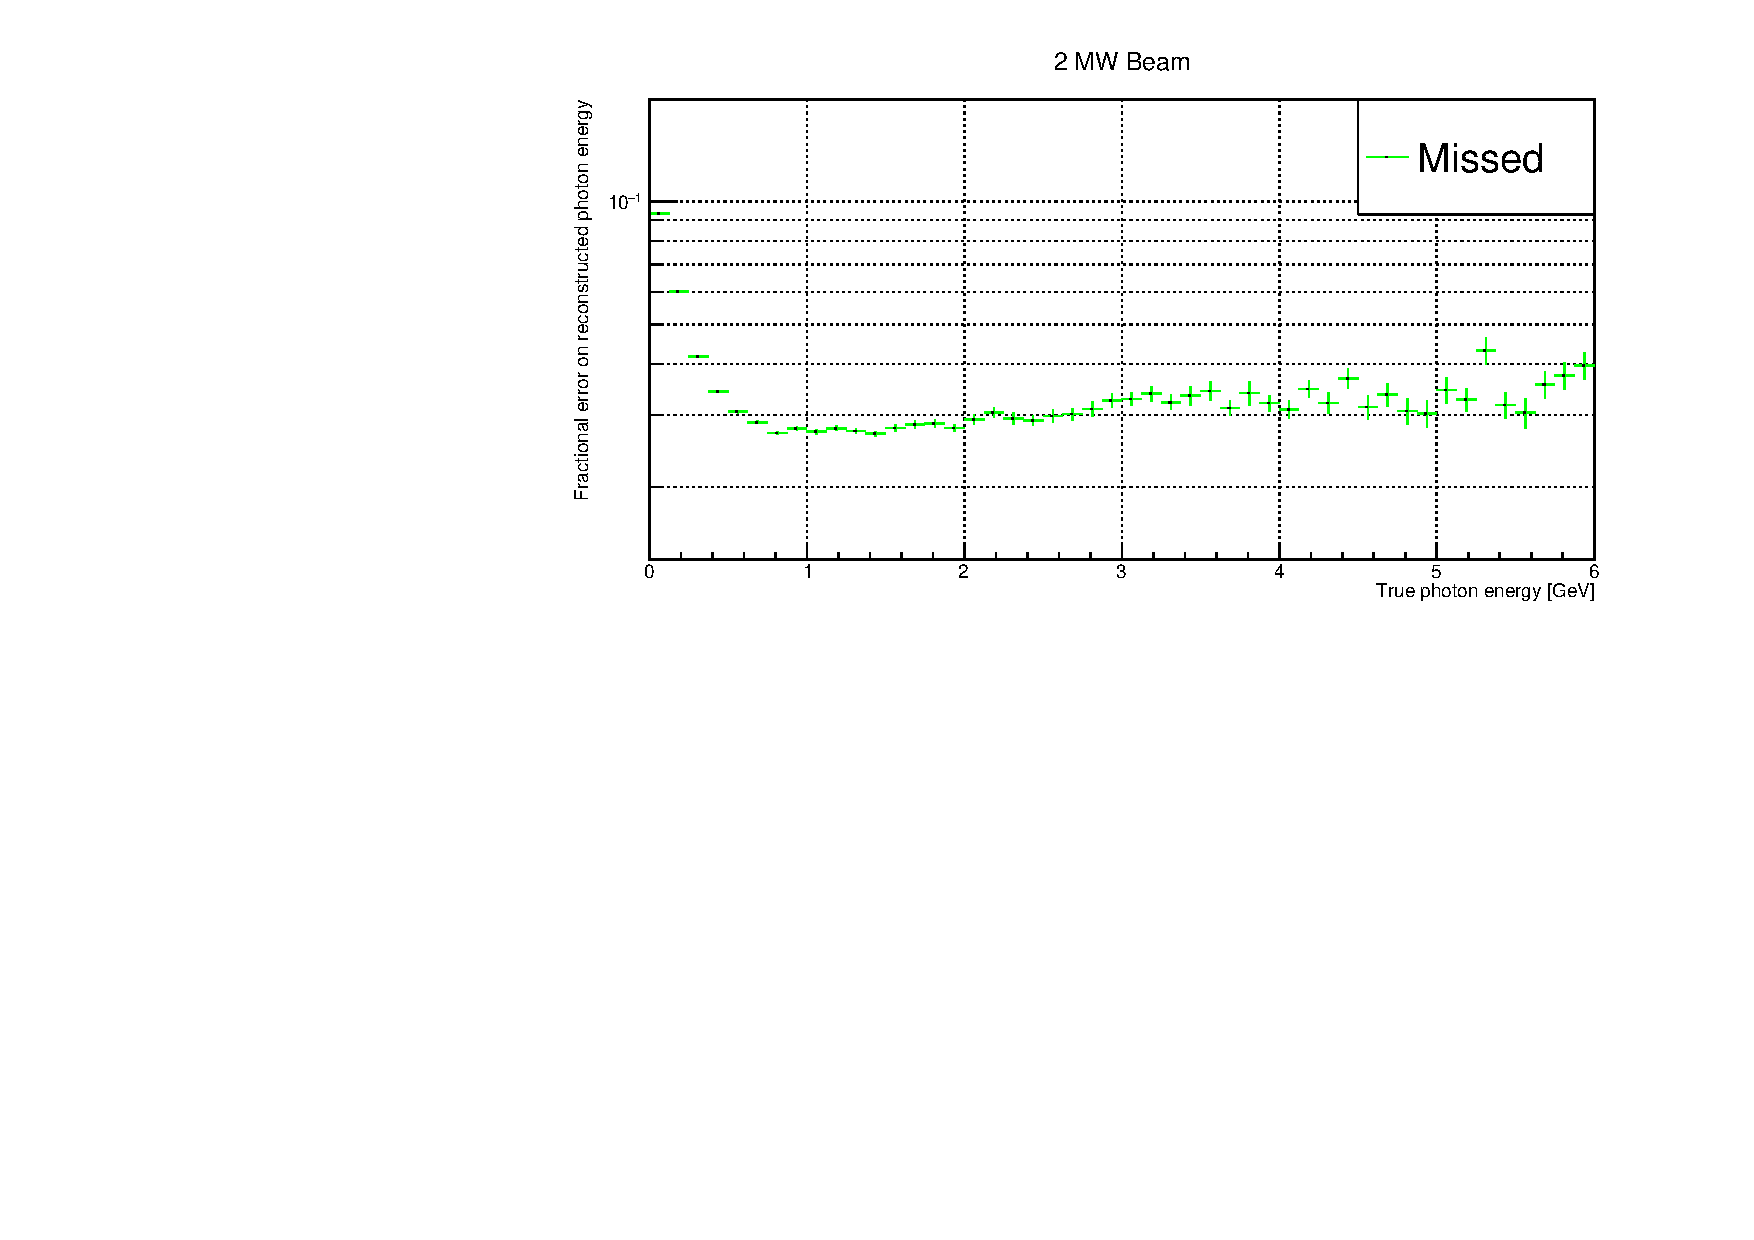
\includegraphics[width=\textwidth]{Figures/2MW/missed_rel_x}
	\caption[Pile-up study mean missed fractional vs.\ true photon energy, \SI{2}{\mega\watt} beam]{%
		Mean missed energy fraction versus true photon energy for a simple $\pi^0$-induced EM shower reconstruction algorithm based on a cone-cylinder union.
		All energy deposited outside of the cone-cylinder union is counted as missed.
		\SI{2}{\mega\watt} beam of \SI{80}{\giga\electronvolt} protons.
	}
	\label{fig:dune-nd_2MW_missed-rel-x}
\end{figure}

It is assumed that EM showers can be identified and their starting point and direction reconstructed with negligible errors and inefficiencies, i.e.\ this information is taken from the truth.
In reality the direction and starting point can be derived from the vertex producing the $\pi^0$, and a rough shower direction obtained from a pattern recognition.
A cone is calculated in the direction of the shower with its tip at the first charge deposition of the initial photon.
The opening angle and length of the cone were optimised by looking at the distributions of the distance from the starting point and the angle w.r.t.\ the direction of the shower.
The finite resolution of the detector is emulated by voxelising (via rounding) the charge deposition with the corresponding resolution in all three spatial coordinates.
This leads to problems near the tip of the cone, where the transversal extent is lower than the voxel dimensions.
In particular, it is possible that the initial charge is shifted outside the cone.
Furthermore, MCS at lower energies makes the cone model suboptimal near the tip.
Therefore, the acceptance volume for the reconstruction is formed of the union of the cone with a cylinder of the same length, along the direction of the shower.
The cylinder radius was tuned to optimise the trade-off between missed and misidentified energy deposition as defined below.

\begin{figure}[tbp]
	\centering
	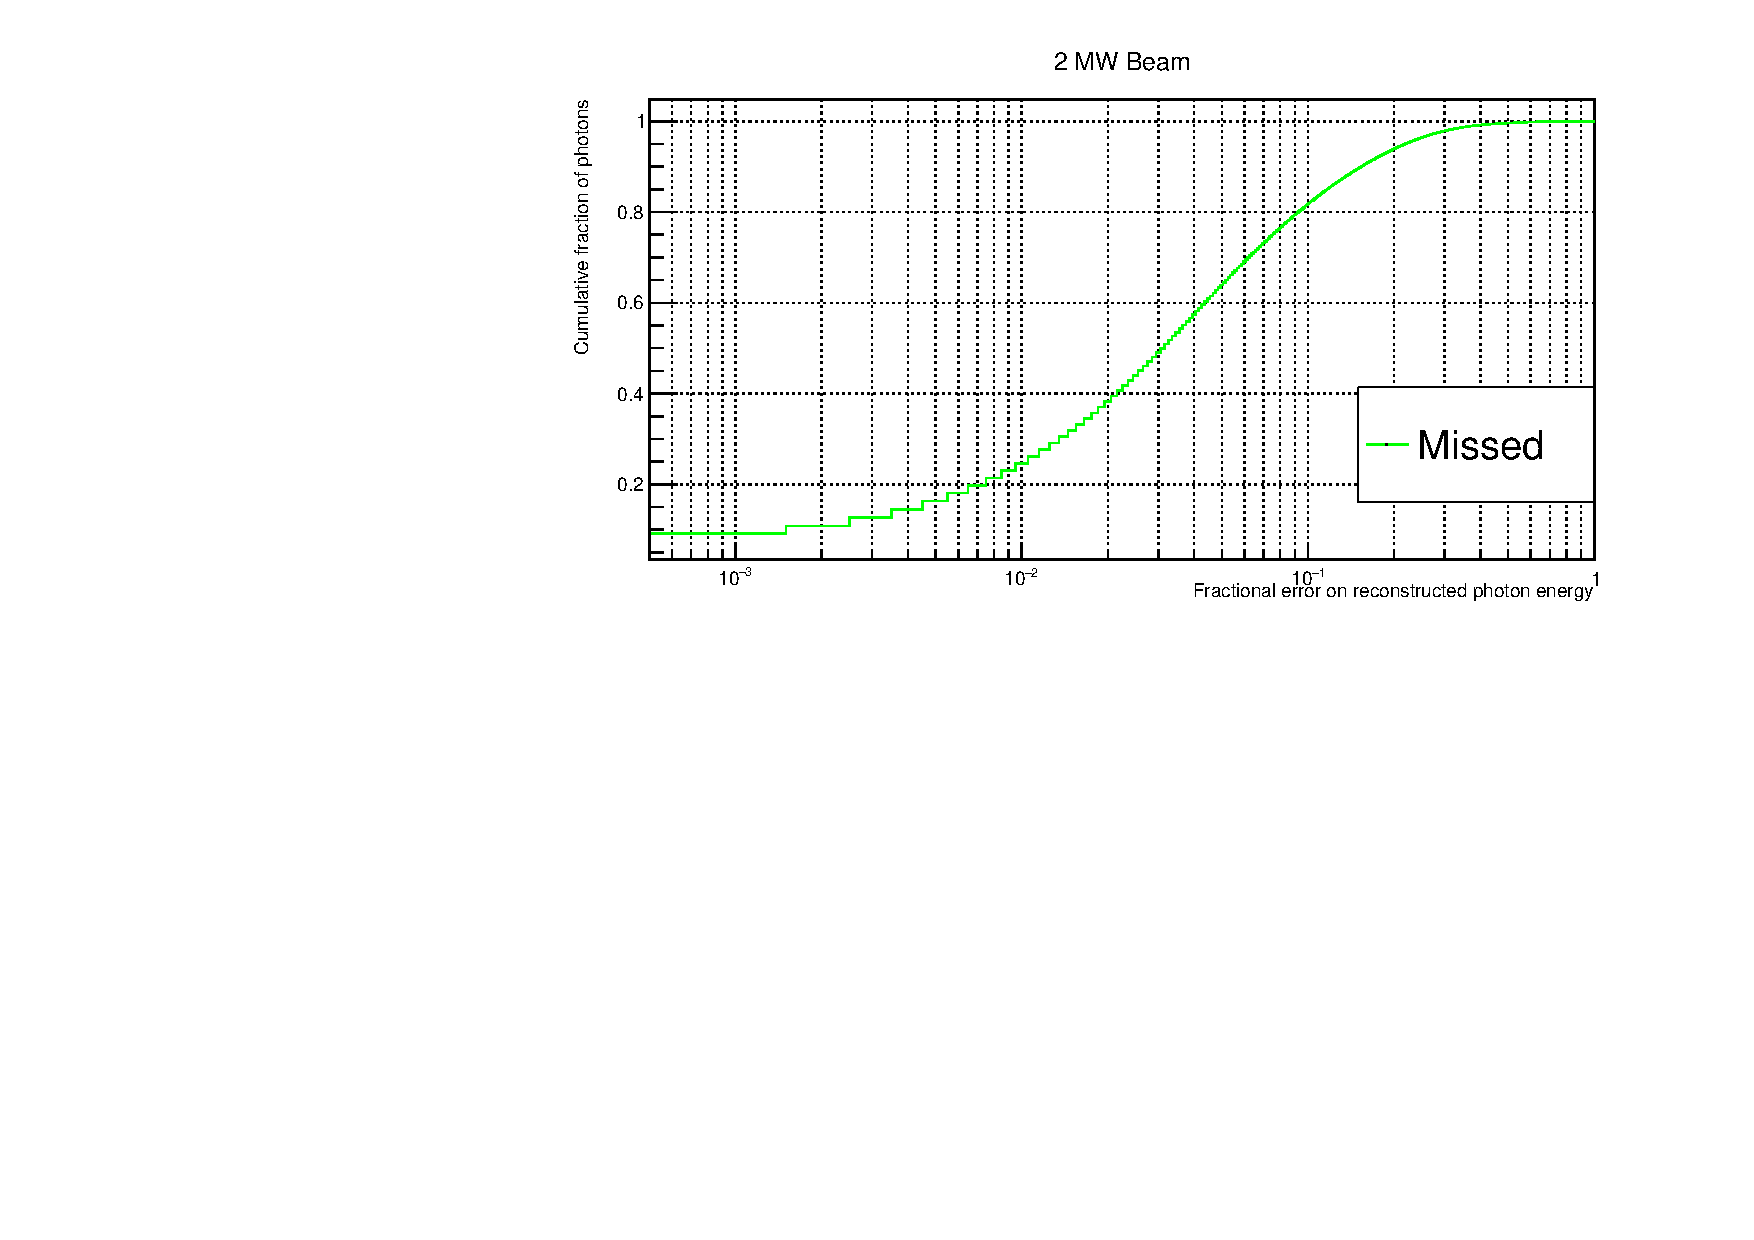
\includegraphics[width=\textwidth]{Figures/2MW/missed_rel_y}
	\caption[Pile-up study photon vs.\ missed energy fraction, \SI{2}{\mega\watt} beam]{%
		Cumulative fraction of photons versus missed energy fraction for a simple $\pi^0$-induced EM shower reconstruction algorithm based on a cone-cylinder union.
		All energy deposited outside of the cone-cylinder union is counted as missed.
		The curve depicts the fraction of photons on the y-axis with a missed energy fraction equal to or lower than the corresponding value on the x-axis.
		\SI{2}{\mega\watt} beam of \SI{80}{\giga\electronvolt} protons.
	}
	\label{fig:dune-nd_2MW_missed-rel-y}
\end{figure}

Argon Box propagates the neutrino interaction events it gets from GENIE through LAr, the output is a ROOT tree of neutrino interaction events.
To get a realistic simulation of beam events in the detector these events need to be distributed randomly in time and space.
Beam spills are simulated by drawing the number of events for each spill from a Poisson distribution whose mean is calculated from the beam intensity and the target mass according~\cite{DUNE3}.
The resulting number of events is taken from the Argon Box ROOT tree and their vertices are placed within the LAr volume at coordinates drawn from a uniform distribution.
Combined with the target mass given in Table~\ref{tab:dune-nd_pile-up-params} this results in an equivalent of $\approx \num{1.5e19}$~POT.
The low number is the result of many neutrino interactions happening outside of the active volume.

\begin{figure}[tbp]
	\centering
	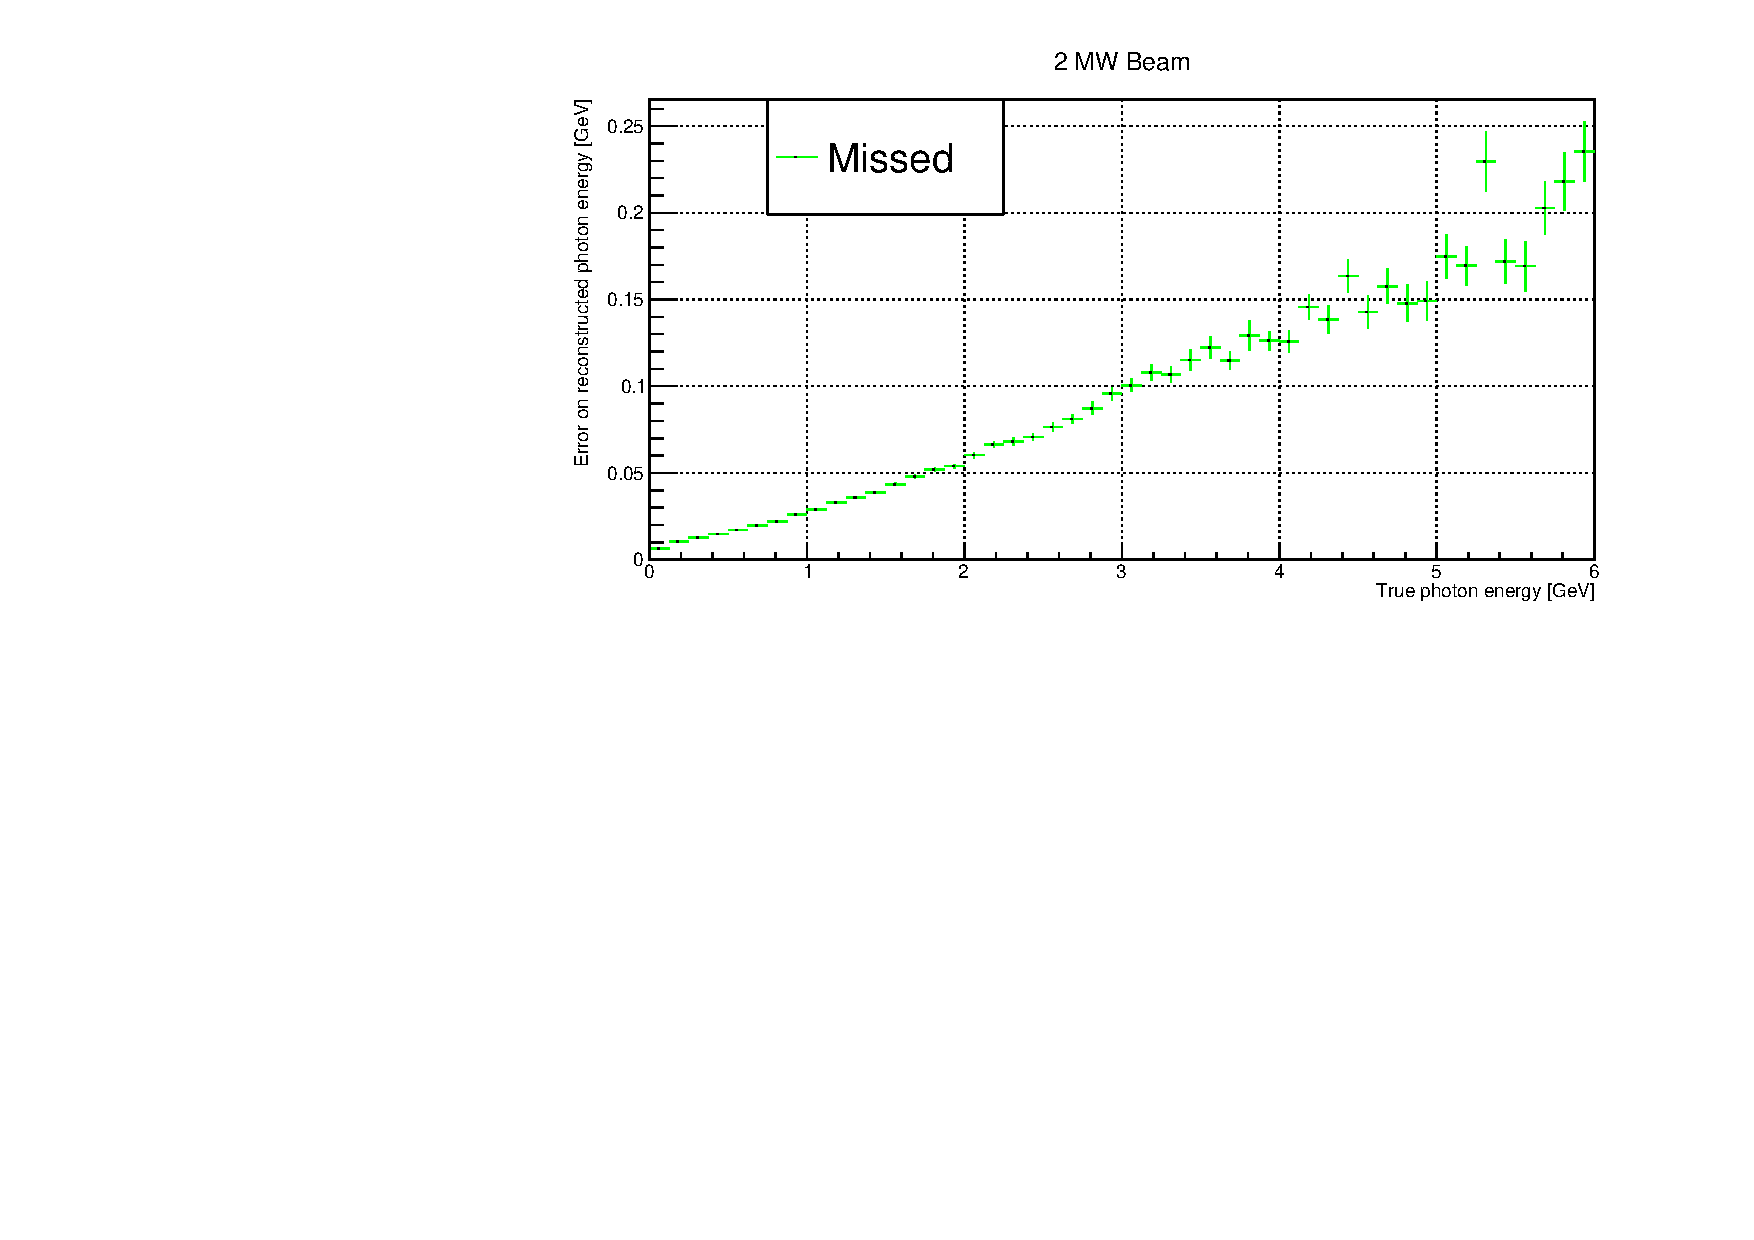
\includegraphics[width=\textwidth]{Figures/2MW/missed_abs_x}
	\caption[Pile-up study mean missed vs.\ true photon energy, \SI{2}{\mega\watt} beam]{%
		Mean missed energy versus true photon energy for a simple $\pi^0$-induced EM shower reconstruction algorithm based on a cone-cylinder union.
		All energy deposited outside of the cone-cylinder union is counted as missed.
		\SI{2}{\mega\watt} beam of \SI{80}{\giga\electronvolt} protons.
	}
	\label{fig:dune-nd_2MW_missed-abs-x}
\end{figure}

Three different argon volumes are assumed for the simulation: target, active, and fiducial volume.
The actual detector dimensions are represented by the active volume.
It is inside the target volume which is the volume within which the neutrino vertices are placed randomly.
This is done to crudely emulate rock events, secondary particles from beam neutrino interactions outside the detector volume.
The additional target mass is \SI{1}{\metre} in all four directions transverse to the beam and \SI{4}{\metre} in upstream beam direction.
According to~\cite{hardon}, hadronic showers up to \SI{10}{\giga\electronvolt} are contained $> \SI{95}{\percent}$ longitudinally and $> \SI{50}{\percent}$ transversally in the additional volume.
Thus, increasing the target volume further will not result in significantly more rock events entering the active volume.
For transversal containment it is enough to use the radius for \SI{95}{\percent} containment because the location of the shower is defined by its centre, i.e.\ showers further away than one \SI{95}{\percent} radius from the detector only deposit a minimal amount of energy inside the detector.
These numbers are supported by the simulations presented in Section~\ref{sec:had_containment}.
EM interactions happen on smaller scales than hadronic interactions, the exception being muons because of their high range.
However, it makes sense to ignore pile-up from muons due to their high reconstruction efficiency.
Finally, a fiducial volume \SI{30}{\centi\metre} ($\approx 2X_0$) smaller than the active volume on all six faces is defined.
Without fiducialising there is a significant number of photons produced by $\pi^0$ decays inside the detector but only showering outside the detector.
This selection results in $\approx \num{5.5e5}$ processed $\pi^0$ photons from the initial \num{6.6e6} neutrino events.
Table~\ref{tab:dune-nd_pile-up-params} contains a summary of all the LAr volume dimensions, Figure~\ref{fig:dune-nd_example-display} shows an example event with all three volumes drawn.

\begin{figure}[tbp]
	\centering
	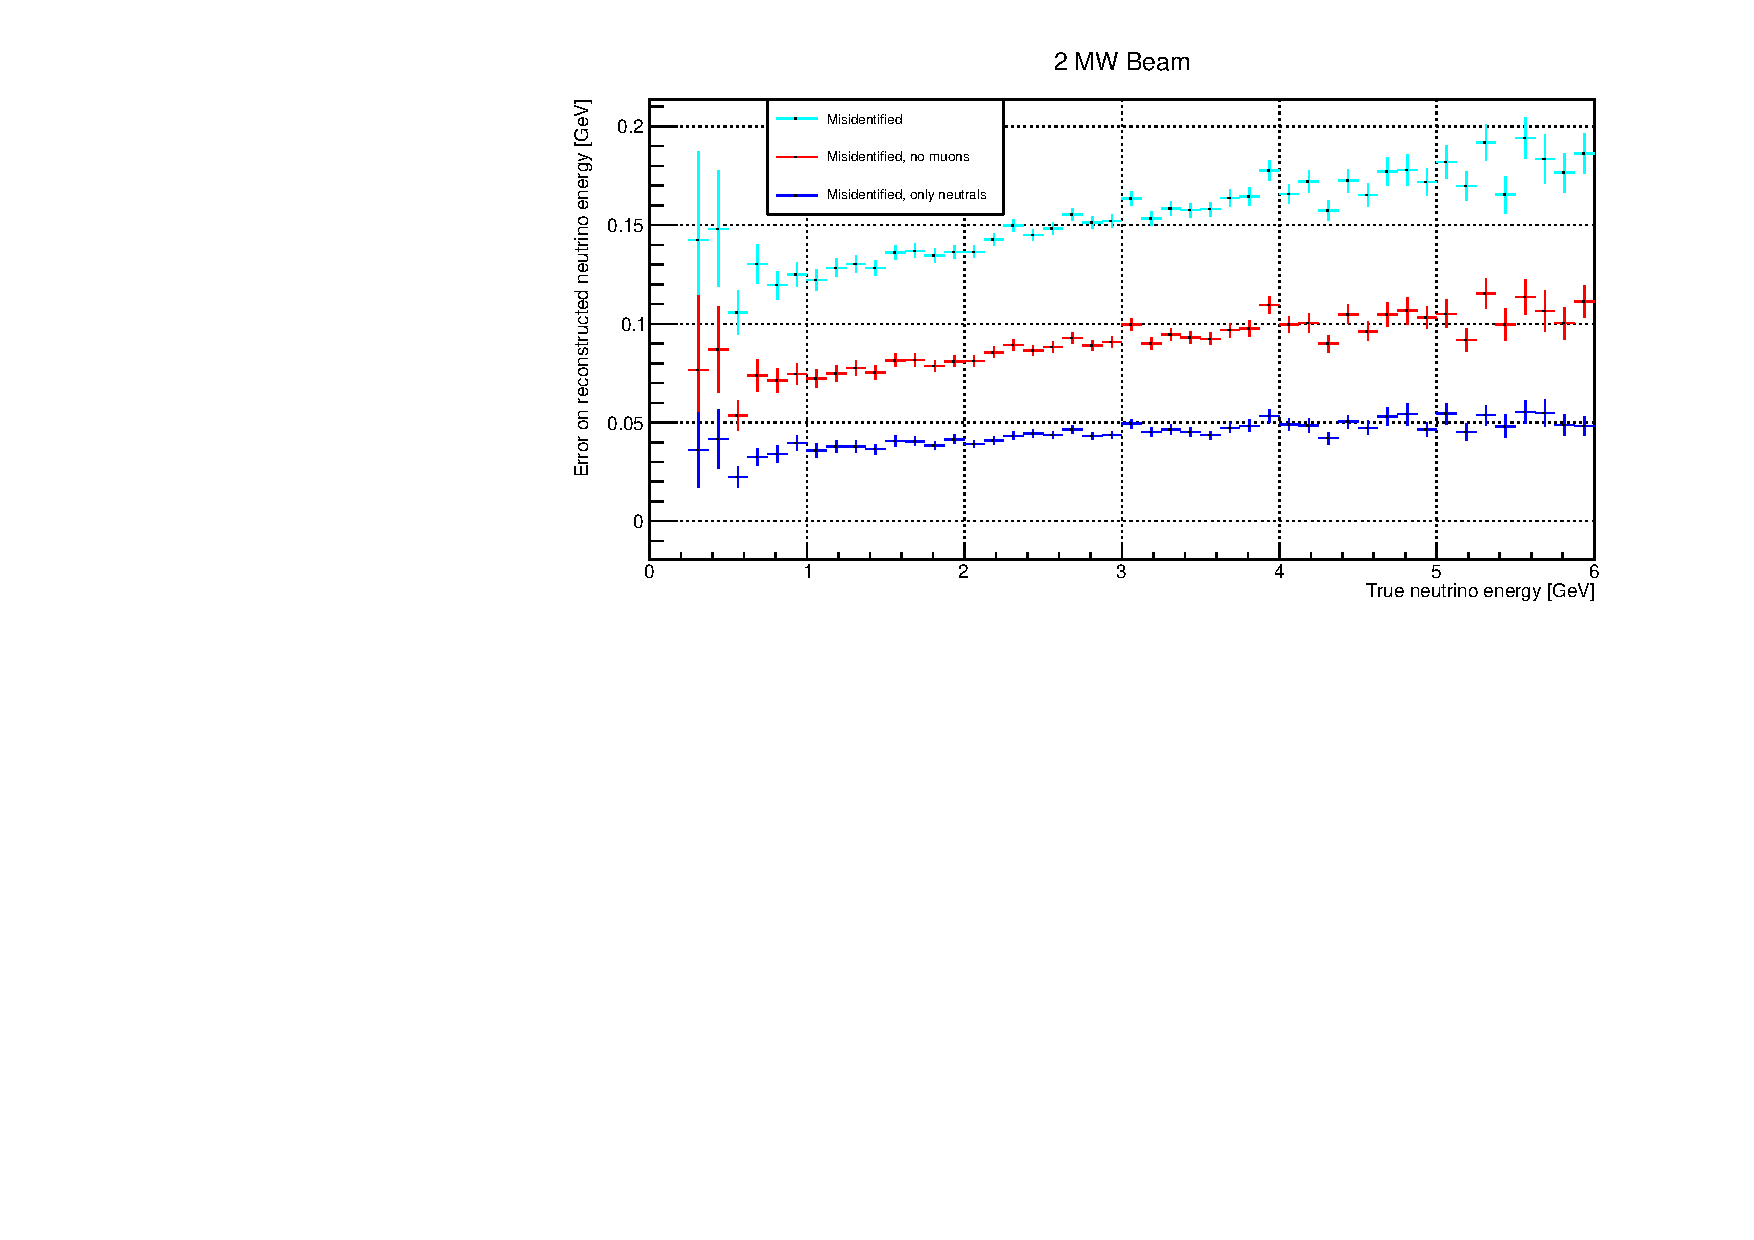
\includegraphics[width=\textwidth]{Figures/2MW/misid_abs_x}
	\caption[Pile-up study mean misidentified vs.\ true neutrino energy, \SI{2}{\mega\watt} beam]{%
		Mean misidentified energy versus true neutrino energy for a simple $\pi^0$-induced EM shower reconstruction algorithm based on a cone-cylinder union.
		All energy deposited inside the cone-cylinder union by descendants of neutrinos different from the parent of the corresponding $\pi^0$ photon is counted as misidentified.
		Colour indicates different selections of misidentified energy: total (cyan); excluding depositions from muons (red); deposition from photons, neutrons, and their descendants only (blue).
		\SI{2}{\mega\watt} beam of \SI{80}{\giga\electronvolt} protons.
	}
	\label{fig:dune-nd_2MW_misid-abs-x}
\end{figure}

Active volume dimensions were taken from the preliminary DUNE ND design; at the time of writing optimal dimensions had not been identified.
Note that the height is \SI{2.5}{\metre} as opposed to the \SI{3}{\metre} of the current ND design.
The reason is that another \SI{0.5}{\metre} safety margin were added after this pile-up simulation had been completed.
The hadron containment studies described in Section~\ref{sec:had_containment} indicated that \SI{2.5}{\metre} height is the bare minimum.
A safety margin was added to account for unknown uncertainties in the simulation.
However, the same simulation framework was used for both the containment and the pile-up study.
Therefore, the \SI{2.5}{\metre} height is sufficient for the pile-up study.

\begin{figure}[tbp]
	\centering
	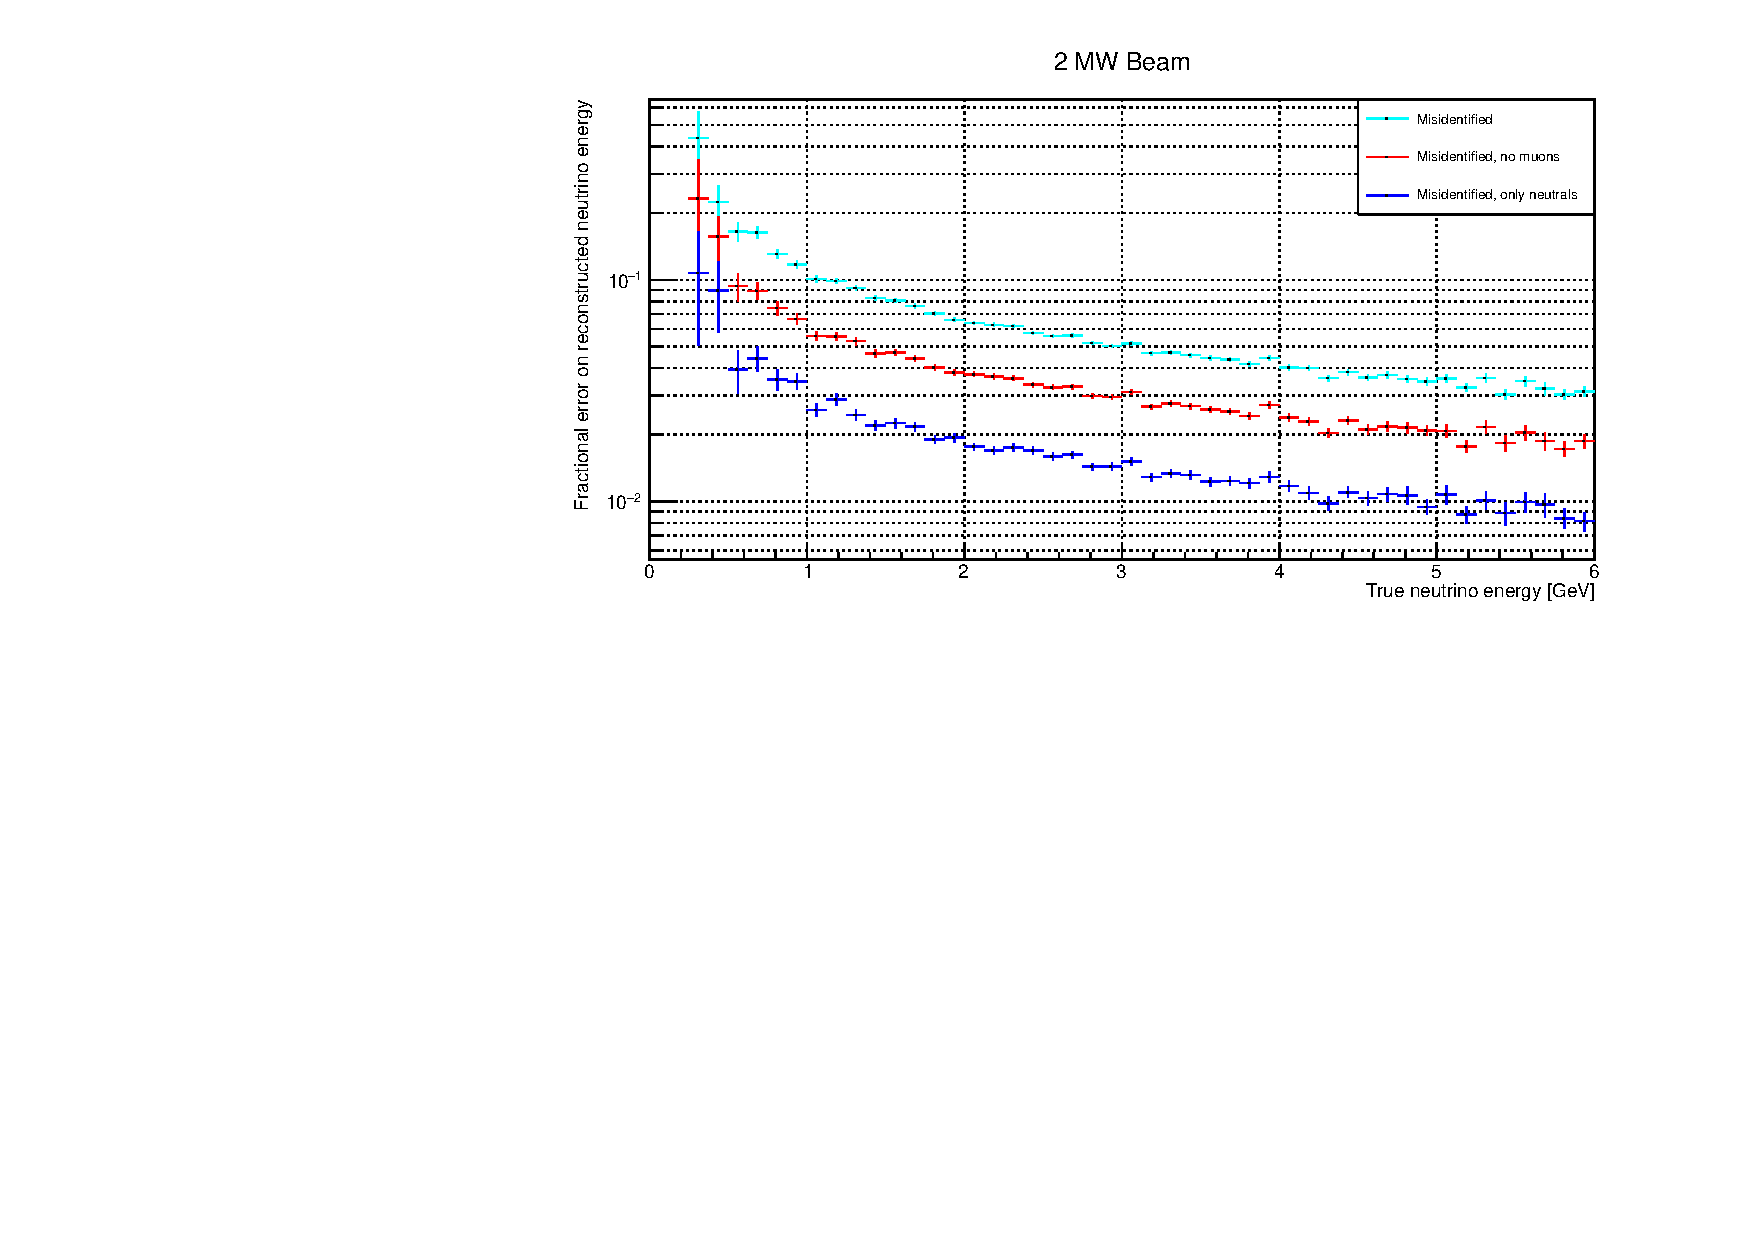
\includegraphics[width=\textwidth]{Figures/2MW/misid_rel_x}
	\caption[Pile-up study mean misidentified fractional vs.\ true neutrino energy, \SI{2}{\mega\watt} beam]{%
		Mean misidentified energy fraction versus true neutrino energy for a simple $\pi^0$-induced EM shower reconstruction algorithm based on a cone-cylinder union.
		All energy deposited inside the cone-cylinder union by descendants of neutrinos different from the parent of the corresponding $\pi^0$ photon is counted as misidentified.
		Colour indicates different selections of misidentified energy: total (cyan); excluding depositions from muons (red); deposition from photons, neutrons, and their descendants only (blue).
		\SI{2}{\mega\watt} beam of \SI{80}{\giga\electronvolt} protons.
	}
	\label{fig:dune-nd_2MW_misid-rel-x}
\end{figure}

Cosmic ray backgrounds are neglected for a number of reasons.
The ND hall will have an overburden of \SI{53}{\metre}, \SI{33}{\metre} of rock (\SI{2.43}{\gram\per\centi\metre\cubed}) plus \SI{20}{\metre} of dirt (\SI{1.7}{\gram\per\centi\metre\cubed}).
Simulations predict a muon rate of \SI{2.7}{\hertz\per\metre\squared} at the top of the hall~\cite{dune_ndtfr}.
Scaled up to the ArC ND footprint of \SI{4 x 5}{\metre}, this results in a rate of \SI{54}{\hertz} for the whole LArTPC component.
However, the majority of these events can be rejected with a beam spill trigger gate.
Looking at Figure~\ref{fig:dune-nd_charge-flux}, the total readout time for one beam spill is \SI{260}{\micro\second}.
Events outside of this window cannot originate from beam neutrinos.
On average this results in \num{0.014} cosmic events per beam spill, compared to \num{14.7} beam events in the simulated detector.


\begin{figure}[tbp]
	\centering
	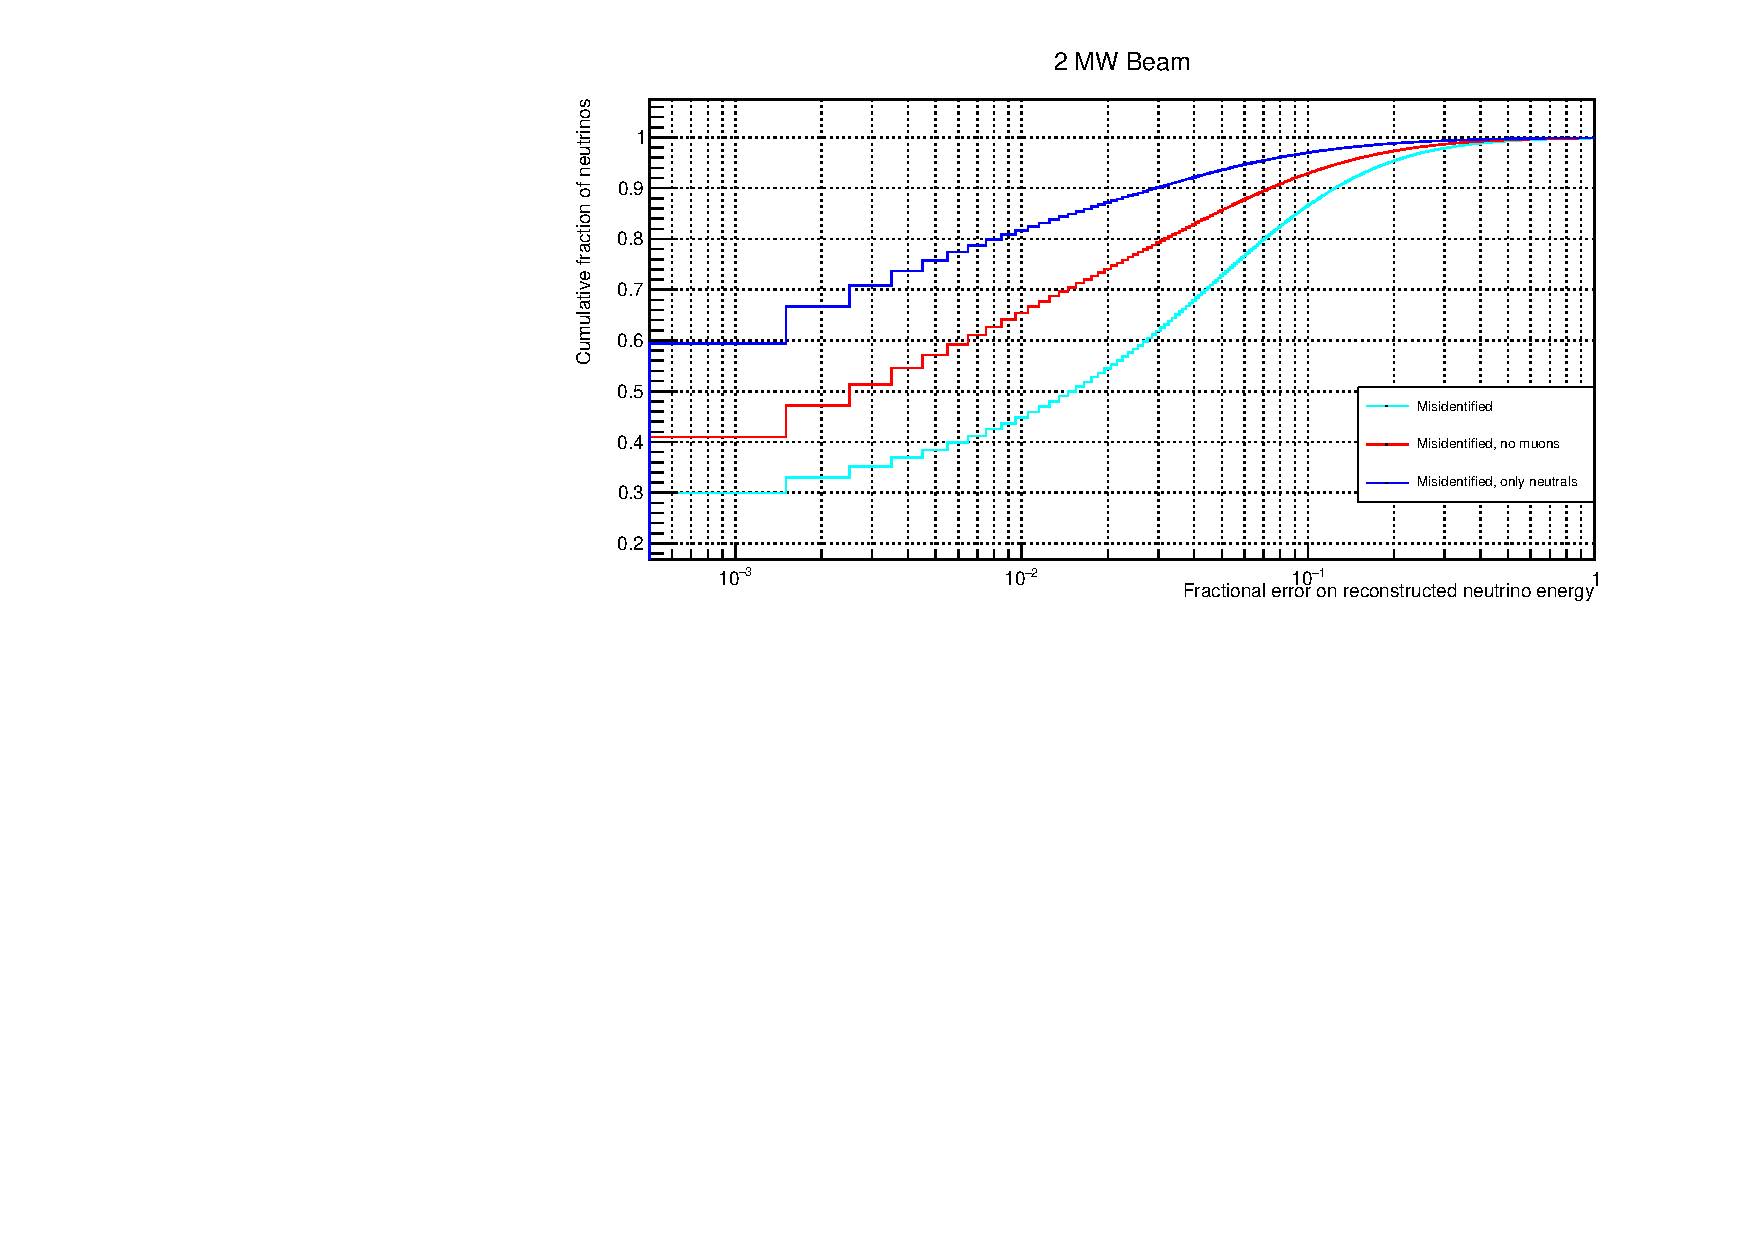
\includegraphics[width=\textwidth]{Figures/2MW/misid_rel_y}
	\caption[Pile-up study neutrino vs.\ misidentified energy fraction, \SI{2}{\mega\watt} beam]{%
		Cumulative fraction of neutrinos versus misidentified energy fraction for a simple $\pi^0$-induced EM shower reconstruction algorithm based on a cone-cylinder union.
		All energy deposited inside the cone-cylinder union by descendants of neutrinos different from the parent of the corresponding $\pi^0$ photon is counted as misidentified.
		Colour indicates different selections of misidentified energy: total (cyan); excluding depositions from muons (red); deposition from photons, neutrons, and their descendants only (blue).
		The curve depicts the fraction of neutrinos on the y-axis with a misidentified energy fraction equal to or lower than the corresponding value on the x-axis.
		\SI{2}{\mega\watt} beam of \SI{80}{\giga\electronvolt} protons.
	}
	\label{fig:dune-nd_2MW_misid-rel-y}
\end{figure}

After all events of one spill are placed inside the target volume, all $\pi^0$ photons produced inside the fiducial volume are reconstructed using the cone-cylinder algorithm.
All energy depositions inside the active volume are considered.
To assess the performance of the algorithm and the influence of pile-up on neutrino energy reconstruction the following two errors on the reconstructed energy are calculated for each $\pi^0$ photon:
\begin{description}
	\item[Missed energy] is the energy deposited by the corresponding $\pi^0$ photon (or its descendants) that is outside the cone-cylinder union and therefore ``missed'' by the algorithm.
	This is a measure of the reconstruction performance and can be used to ensure optimum tuning of the union parameters.
	\item[Misidentified energy] is the energy inside the cone-cylinder union deposited by descendants of a different (``wrong'') parent neutrino.
	This is a measure of event pile-up: the higher the charge deposition by other events inside the union, the higher the event pile-up.
\end{description}
Using this general definition of misidentified energy leads to quite mediocre results.
However, there are some assumptions that can be taken even without knowing the actual reconstruction algorithm.
From MicroBooNE~\cite{pandora} the muon reconstruction can be assumed to be very efficient.
Assuming \SI{100}{\percent} reconstruction efficiency for muons and \SI{0}{\percent} for all other particles provides an upper limit for misidentified energy.
Which can be calculated by ignoring energy deposited by muons originating from other parent neutrinos.
A lower limit for misidentified energy can be calculated by assuming \SI{100}{\percent} reconstruction efficiency for all charged particles and \SI{0}{\percent} for neutral particles ($\gamma$ and $n$).
This is calculated by only taking into account misidentified energy deposited by neutral particles.
Even assuming \SI{0}{\percent} reconstruction efficiency for neutral particles is potentially too pessimistic.
Future, more sophisticated reconstruction algorithms (e.g.\ based on machine learning) might be able to partially reconstruct the topology of charge depositions originating from neutral particles and thus prevent their misidentification.
Therefore, it can be assumed that the actual pile-up-related energy reconstruction error is closer to the lower limit and potentially even below.
It should be noted that the upper limit excludes only energy deposited by muons directly and not by their descendants (e.g.\ $\delta$ rays or Michel electrons).
Whereas, the lower limit excludes charge deposited by photons, neutrons, and any of their descendants.
Figure~\ref{fig:dune-nd_example-display-zoom} illustrates the distinction of various energy depositions for an example event.
In particular, it can be seen that $\delta$ rays (orange) are not counted towards energy deposited by muons (yellow).
The long red track is an example of a deposition originating from a photon or neutron (descendant) included in the lower limit sample but very likely reconstructible by future algorithms.

Missed and misidentified energy by the cone-cylinder union are analysed as a function of true photon and neutrino energy, respectively.
As mentioned above, the missed energy is used to measure the performance of the reconstruction algorithm.
Therefore, it is sensible to compare it to the true photon energy rather than the true energy of its parent neutrino.
However, the primary goal of this study is to assess the effect of event pile-up on the neutrino energy spectrum.
The misidentified energy is thus compared to the true neutrino energy.
Therefore, the total misidentified energy of each neutrino event is first calculated by summing up the contributions of all descending $\pi^0$ photons.
It is also illustrative to look at the fraction of events with a certain misidentified or missed energy.
For misidentified energy this is the fraction of neutrino events containing $\pi^0$-induced EM showers, not the fraction of all neutrino events.
All the aforementioned information is contained in 2D histograms of all events with the true neutrino (photon) energy on one axis and the misidentified (missed) energy on the other axis.
The energy dependence of the error can be obtained by looking at the true energy axis and calculating the mean misidentified (missed) energy for each bin (a profile of the 2D histogram).
Looking at the misidentified (missed) energy axis and summing over all true energy bins yields the number of events with the corresponding misidentified (missed) energy (a projection of the 2D histogram).
The corresponding fraction of events is obtained by normalising the histogram.
For the profiles, only events with energies from \SIrange{0}{6}{\giga\electronvolt} or energy fractions from \numrange{0}{1} are taken into account.

The results for a \SI{2}{\mega\watt} beam at \SI{80}{\giga\electronvolt} proton energy are shown in Figures~\ref{fig:dune-nd_2MW_rel-2d-missed} through~\ref{fig:dune-nd_2MW_misid-rel-y}.
To illustrate the relation between the different histograms all of them are shown for the missed energy in Figures~\ref{fig:dune-nd_2MW_rel-2d-missed} through~\ref{fig:dune-nd_2MW_missed-rel-y}.
The initial 2D histogram is shown in Figure~\ref{fig:dune-nd_2MW_rel-2d-missed}.
Note that it actually depicts the missed photon energy as a fraction of the true photon energy rather than an absolute value.
Figure~\ref{fig:dune-nd_2MW_missed-rel-x} is the profile of the x-axis, i.e.\ the mean missed energy fraction for each true energy bin.
The projection of the y-axis is depicted in Figure~\ref{fig:dune-nd_2MW_missed-rel-y}.
This is the fraction of photons with a certain missed energy.
It is drawn as a cumulative fraction, which means that the curve represents the fraction of photons on the y-axis with a missed energy fraction equal to or lower than the corresponding value on the x-axis.
A consequence of this is that the curve monotonically approaches one towards the right, \SI{100}{\percent} of the reconstructed photons have a missed energy fraction of \SI{100}{\percent} or less.
For reference Figure~\ref{fig:dune-nd_2MW_missed-abs-x} shows the mean absolute missed energy per true energy bin.

It can be seen that the absolute missed energy rises more or less linearly with the true energy (Figure~\ref{fig:dune-nd_2MW_missed-abs-x}), indicating that the cone models the shower well.
Indeed, it can be seen from Figure~\ref{fig:dune-nd_2MW_missed-rel-x} that the missed energy fraction stays almost constant at \SI{3}{\percent} from \SIrange{1}{6}{\giga\electronvolt}.
It starts to increase below \SI{1}{\giga\electronvolt}, reaching almost \SI{10}{\percent} in the lowest energy bin (\SIrange{0}{125}{\mega\electronvolt}).
This can be explained by the increase in MCS at lower momenta.
The Compton scattering cross-section increases in a similar way.
Both these effects lead to a higher angular distribution of the energy deposited by electrons (and positrons) and photons.
Consequentially, more energy is missed because the cone angle is independent of energy.
From Figure~\ref{fig:dune-nd_2MW_missed-rel-y} it can be seen that for roughly half of the photons \SI{3}{\percent} of the energy is missed, indicating a symmetric distribution of missed energy around the mean value.
It should be noted that "leakage" energy deposited outside the detector is included in the missed energy.
Despite the fiducial volume some events still exit the detector.

\begin{figure}[tbp]
	\centering
	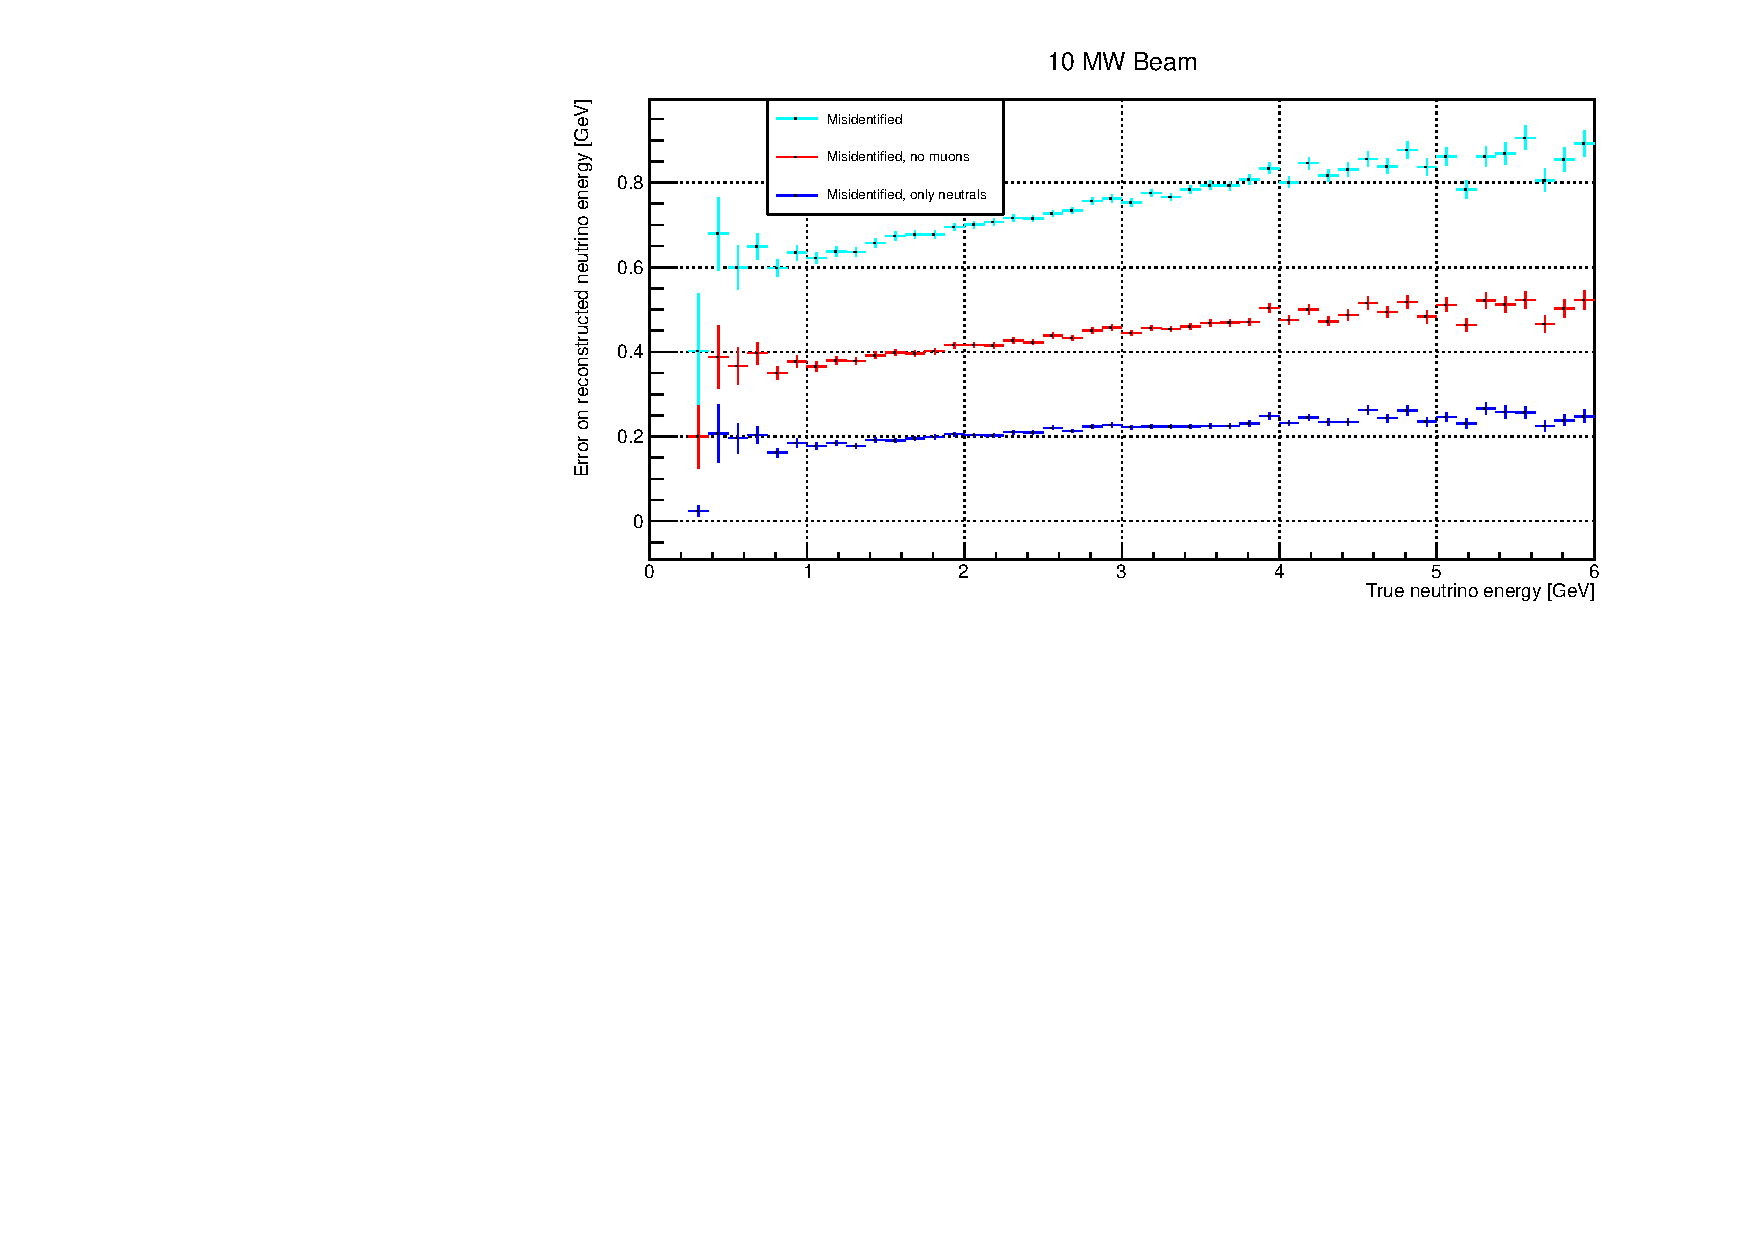
\includegraphics[width=\textwidth]{Figures/10MW/misid_abs_x}
	\caption[Pile-up study mean misidentified vs.\ true neutrino energy, \SI{10}{\mega\watt} beam]{%
		Mean misidentified energy versus true neutrino energy for a simple $\pi^0$-induced EM shower reconstruction algorithm based on a cone-cylinder union.
		All energy deposited inside the cone-cylinder union by descendants of neutrinos different from the parent of the corresponding $\pi^0$ photon is counted as misidentified.
		Colour indicates different selections of misidentified energy: total (cyan); excluding depositions from muons (red); deposition from photons, neutrons, and their descendants only (blue).
		\SI{10}{\mega\watt} beam of \SI{80}{\giga\electronvolt} protons.
	}
	\label{fig:dune-nd_10MW_misid-abs-x}
\end{figure}

The behaviour of the misidentified energy is almost opposite to the missed energy:
The absolute value is nearly constant with the true neutrino energy (Figure~\ref{fig:dune-nd_2MW_misid-abs-x}) while the fraction of the total energy is inversely proportional to the true energy, accordingly (Figure~\ref{fig:dune-nd_2MW_misid-rel-x}).
This is expected as the amount of charge deposited inside the cone originating from other neutrinos should only depend on the geometry of the acceptance volume  and on the event rate, but not on the true energy of the reconstructed photon or its parent neutrino.
The effect of the different misidentified energy selections can be seen well.
As mentioned, the actual error on the reconstructed neutrino energy is probably somewhere in between the red curve, only rejecting misidentified energy deposited by muons, and the dark blue curve, rejecting all but misidentified energy deposited by photons and neutrons or any of their descendants.
From Figure~\ref{fig:dune-nd_2MW_misid-rel-x} this can be determined to be about \SIrange{2}{3}{\percent} at the flux peak $\approx \SI{2.5}{\giga\electronvolt}$.
The cumulative neutrino fraction versus the misidentified energy fraction shows that about \SI{70}{\percent} of the events experience a pile-up-related error on reconstructed neutrino energy of \SI{1}{\percent} or less.
For roughly \SI{50}{\percent} of the events it is even below \SI{0.1}{\percent}.
If it was possible to identify this \SI{50}{\percent} in the real experiment, they could be cut, giving an essentially pile-up-free sample.
This would be easily affordable given the high event rates in the ND, see Section~\ref{sec:rates}.
In the case of the algorithm described here, EM shower pile-up could be detected via overlapping cones for instance.

\begin{figure}[tbp]
	\centering
	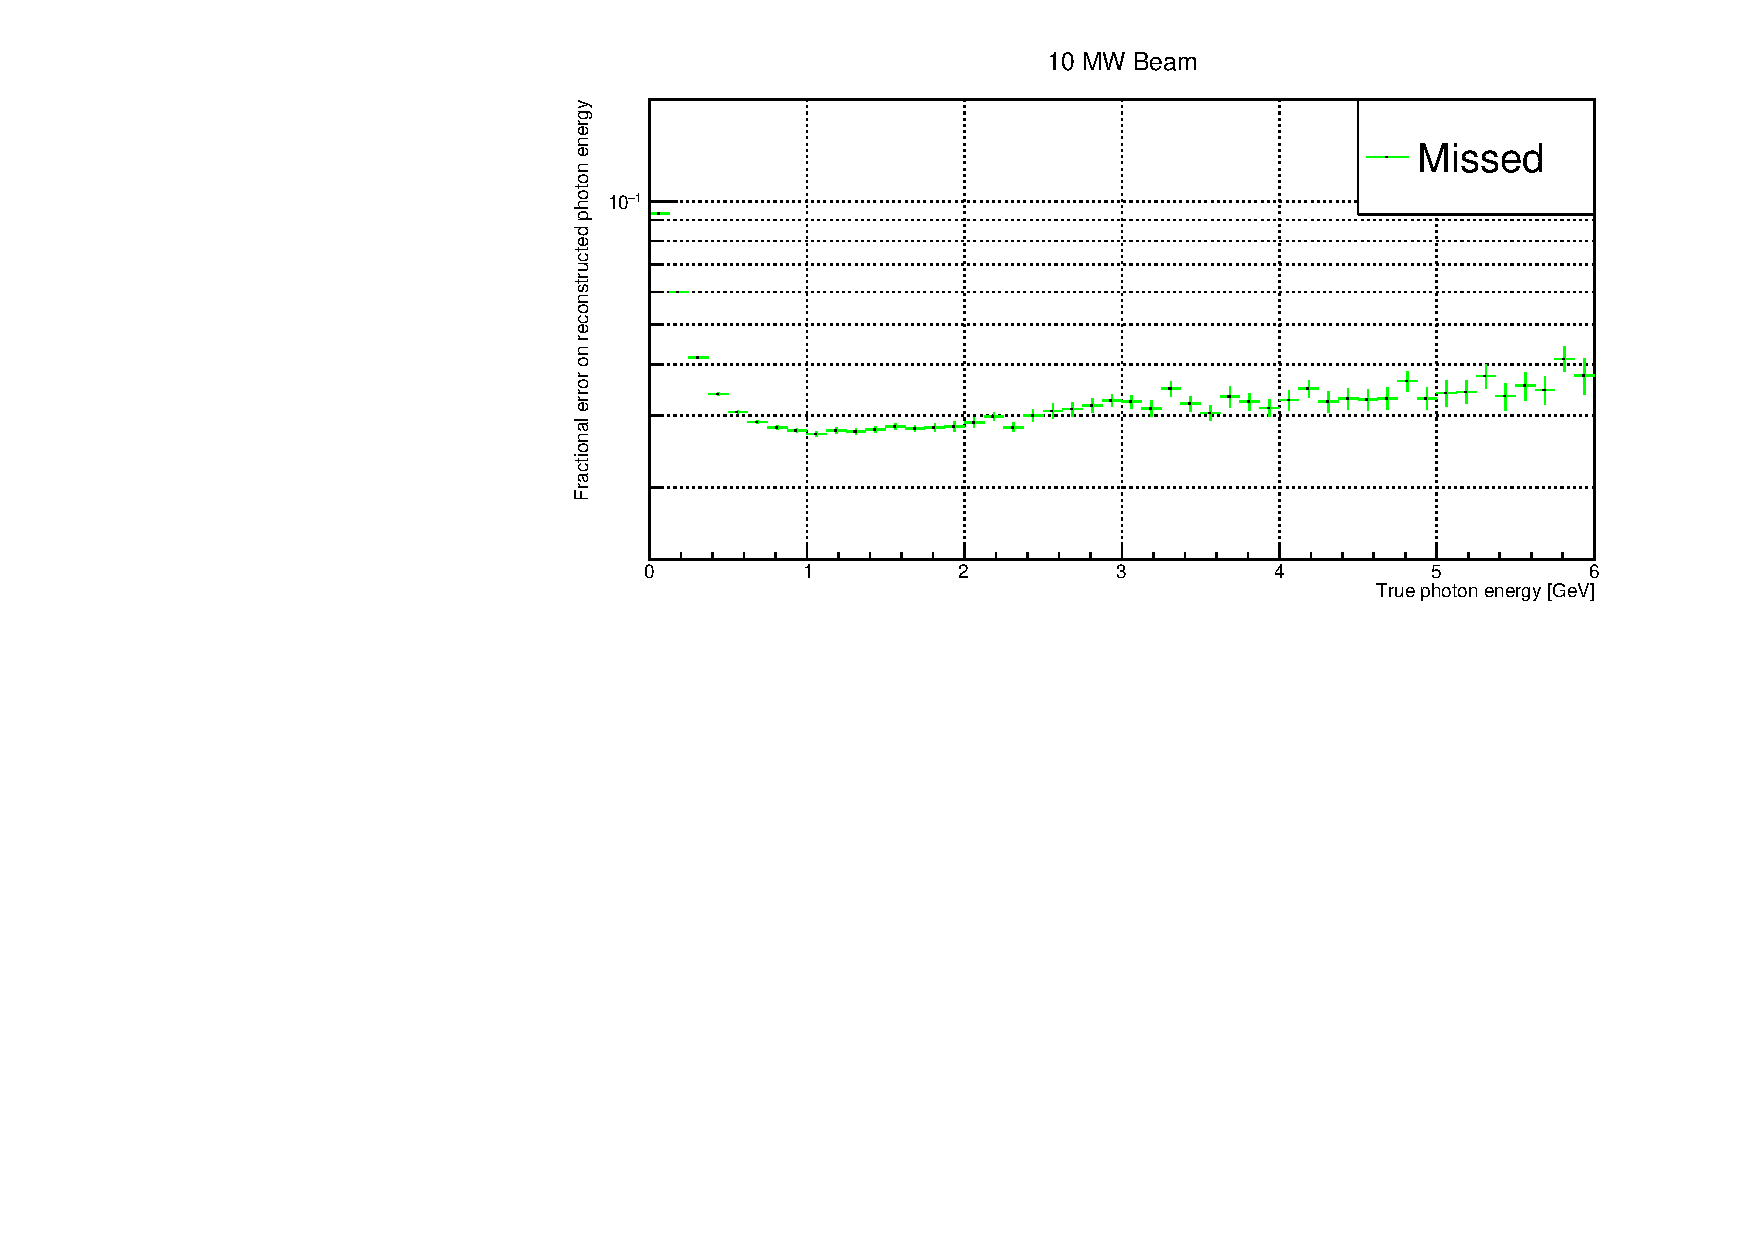
\includegraphics[width=\textwidth]{Figures/10MW/missed_rel_x}
	\caption[Pile-up study mean missed fractional vs.\ true photon energy, \SI{10}{\mega\watt} beam]{%
		Mean missed energy fraction versus true photon energy for a simple $\pi^0$-induced EM shower reconstruction algorithm based on a cone-cylinder union.
		All energy deposited outside of the cone-cylinder union is counted as missed.
		\SI{10}{\mega\watt} beam of \SI{80}{\giga\electronvolt} protons.
	}
	\label{fig:dune-nd_10MW_missed-rel-x}
\end{figure}

Finally, as a cross-check the pile-up study was performed for a hypothetical \SI{10}{\mega\watt} beam in Figures~\ref{fig:dune-nd_10MW_missed-rel-x} through~\ref{fig:dune-nd_10MW_misid-rel-y}.
As explained, the missed energy only depends on the geometry of the acceptance volume, it should be independent of beam intensity.
It is therefore expected to be very similar to the \SI{2}{\mega\watt} case, confirmed by comparing Figure~\ref{fig:dune-nd_10MW_missed-rel-x} to Figure~\ref{fig:dune-nd_2MW_missed-rel-x}.
As expected, the error due to misidentified energy is increased to \SIrange{8}{15}{\percent} at the flux peak (Figure~\ref{fig:dune-nd_10MW_misid-rel-x}).
Similarly, only about \SI{10}{\percent} of the neutrino events remain pile-up free while \SI{50}{\percent} suffer from more than \SI{4}{\percent} misidentified energy (Figure~\ref{fig:dune-nd_10MW_misid-rel-y}).

\begin{figure}[tbp]
	\centering
	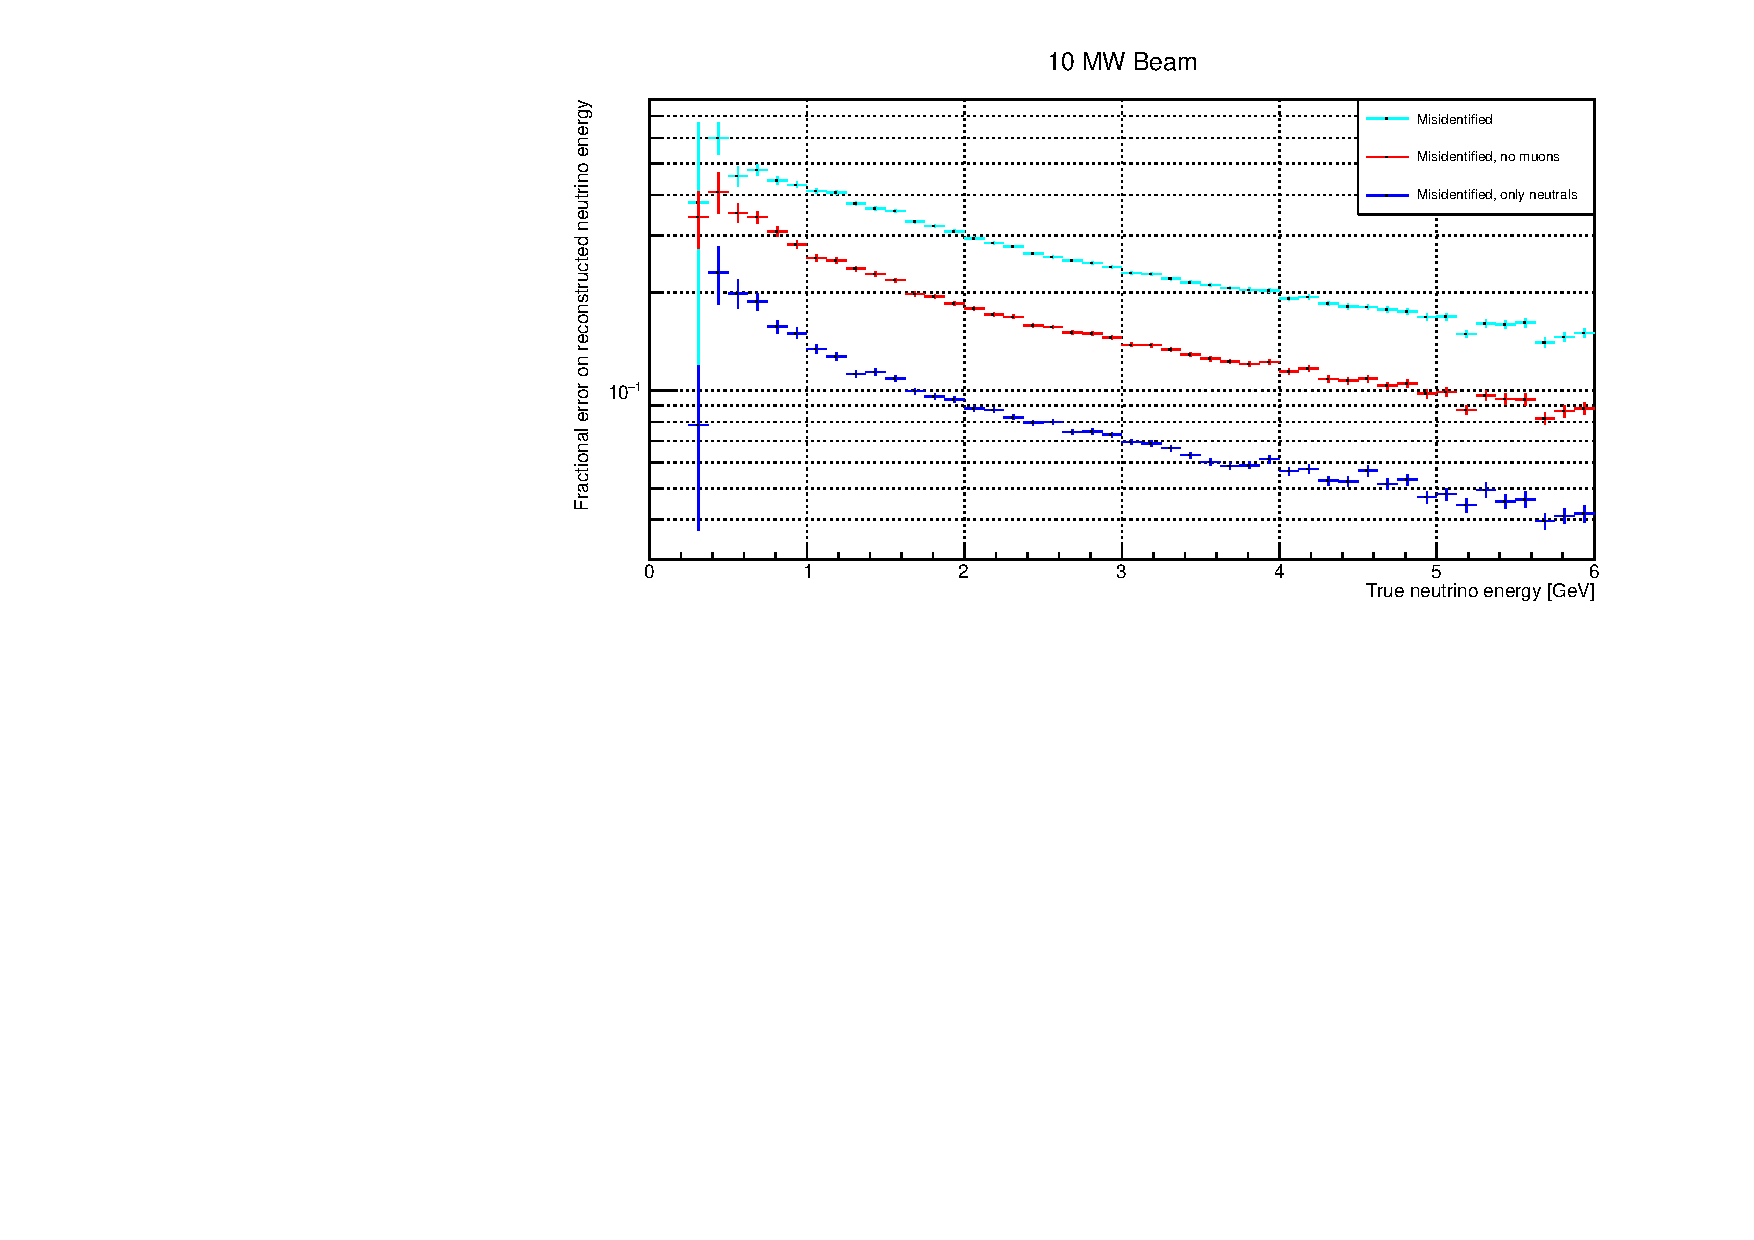
\includegraphics[width=\textwidth]{Figures/10MW/misid_rel_x}
	\caption[Pile-up study mean misidentified fractional vs.\ true neutrino energy, \SI{10}{\mega\watt} beam]{%
		Mean misidentified energy fraction versus true neutrino energy for a simple $\pi^0$-induced EM shower reconstruction algorithm based on a cone-cylinder union.
		All energy deposited inside the cone-cylinder union by descendants of neutrinos different from the parent of the corresponding $\pi^0$ photon is counted as misidentified.
		Colour indicates different selections of misidentified energy: total (cyan); excluding depositions from muons (red); deposition from photons, neutrons, and their descendants only (blue).
		\SI{10}{\mega\watt} beam of \SI{80}{\giga\electronvolt} protons.
	}
	\label{fig:dune-nd_10MW_misid-rel-x}
\end{figure}

In summary, even a very simple EM shower reconstruction algorithm, employing a cone-cylinder union selection, performs well in the high-multiplicity environment of the DUNE ND, when fed with unambiguous 3D spatial coordinates of energy deposits.
The mean deposited energy missed by the algorithm is less than \SI{3}{\percent}.
More importantly, the pile-up-related misidentification of energy depositions from other events has a mean of \SIrange{2}{3}{\percent}.
For more than \SI{50}{\percent} of the neutrino events containing $\pi^0$-induced EM showers this error is even smaller than \SI{0.1}{\percent}.
If a method is developed to flag the other \SI{50}{\percent} as piled up during reconstruction, a sample of neutrino events almost free of pile-up can be generated.
In comparison, the FD is required to have an energy resolution for stopping hadrons below \SI{10}{\percent} and an electron energy resolution of $\SI{1}{\percent} \oplus \SI{15}{\percent} \times \sqrt{\frac{\SI{1}{\mega\electronvolt}}{E}}$~\cite{dune4}.
Provided that a successful LArPix enables unambiguous 3D tracking information, ArC will be capable of handling the high rates expected in the DUNE ND environment without significant contributions to the error budget.
The employed reconstruction algorithm clearly fails when confronted with a much higher beam intensity.

\begin{figure}[tbp]
	\centering
	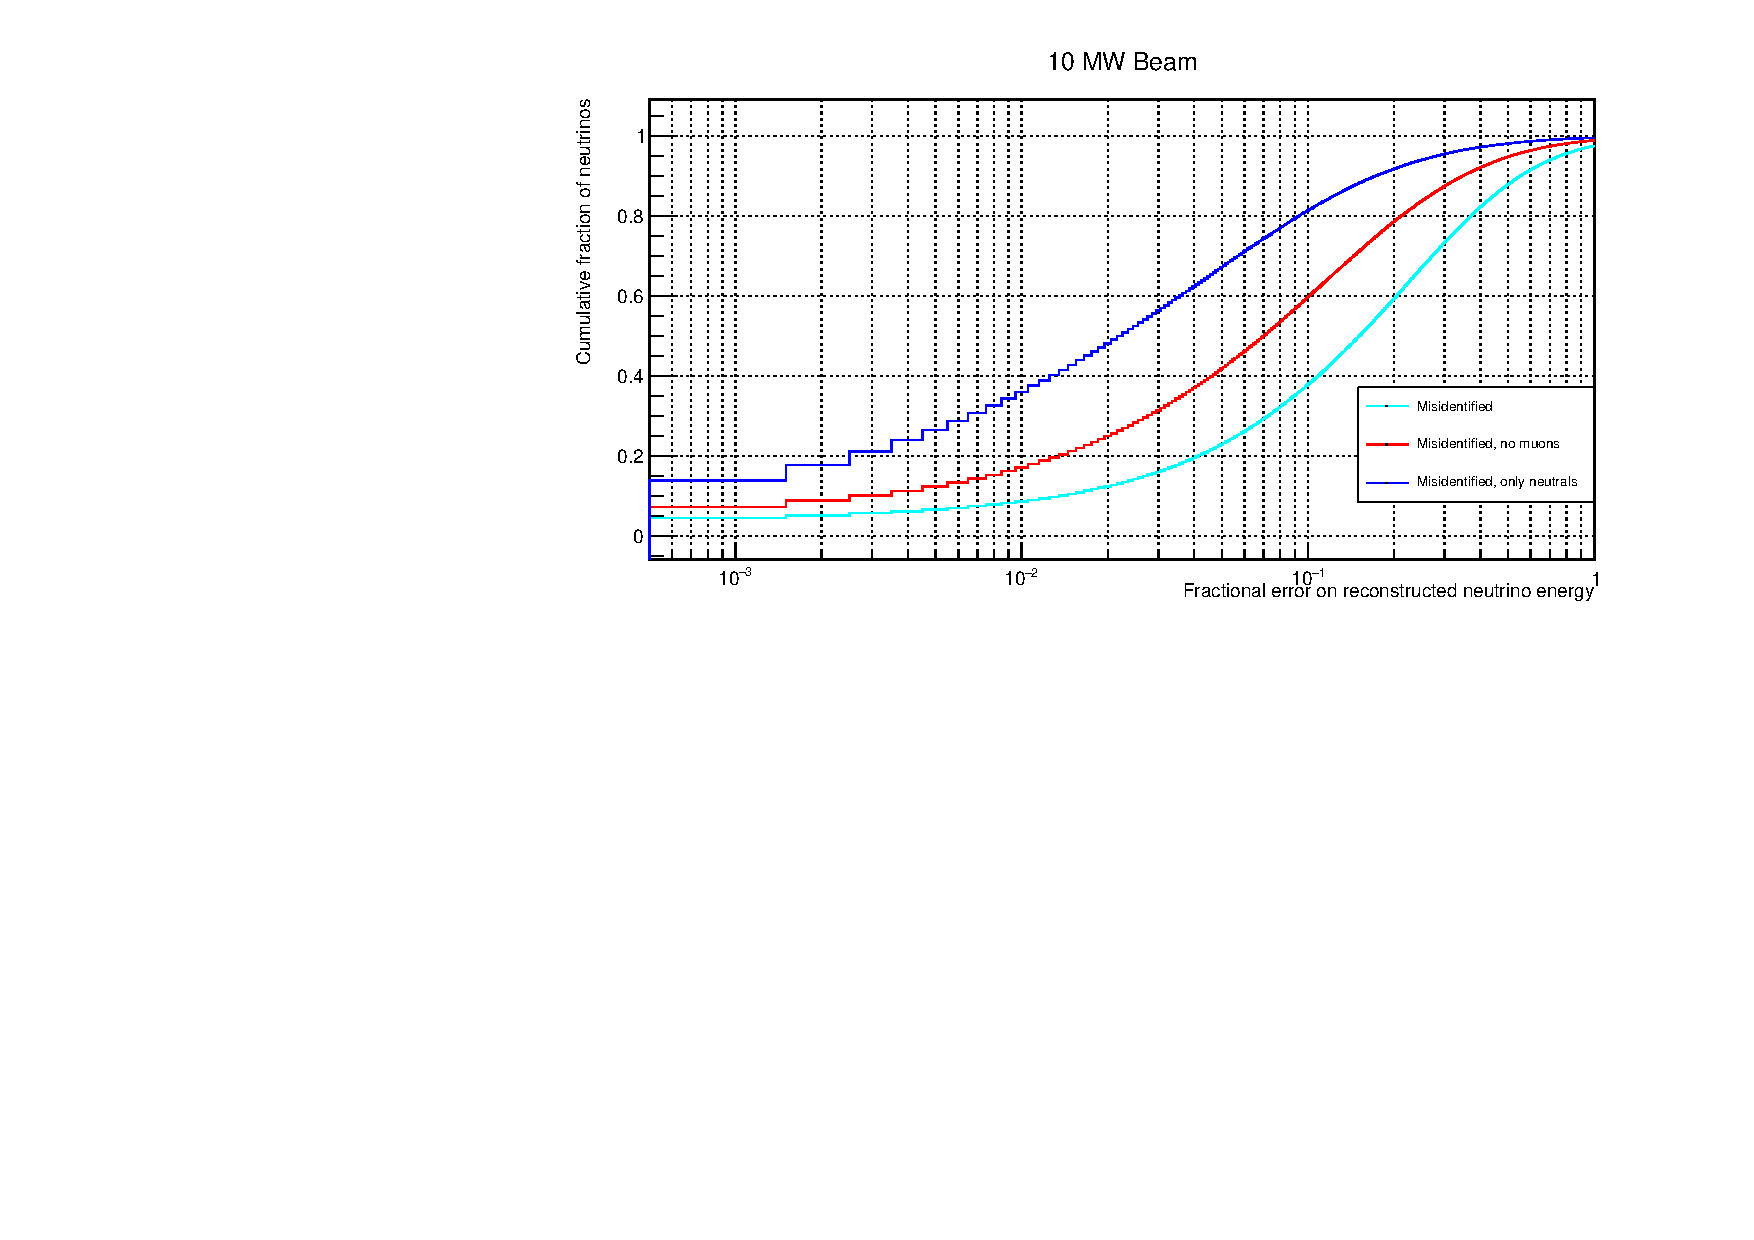
\includegraphics[width=\textwidth]{Figures/10MW/misid_rel_y}
	\caption{Cumulative fraction of neutrinos versus misidentified energy fraction for a simple $\pi^0$-induced EM shower reconstruction algorithm based on a cone-cylinder union.
		All energy deposited inside the cone-cylinder union by descendants of neutrinos different from the parent of the corresponding $\pi^0$ photon is counted as misidentified.
		Colour indicates different selections of misidentified energy: total (cyan); excluding depositions from muons (red); deposition from photons, neutrons, and their descendants only (blue).
		The curve depicts the fraction of neutrinos on the y-axis with a misidentified energy fraction equal to or lower than the corresponding value on the x-axis.
		\SI{10}{\mega\watt} beam of \SI{80}{\giga\electronvolt} protons.
	}
	\label{fig:dune-nd_10MW_misid-rel-y}
\end{figure}


\section{Neutrino-Electron Elastic Scattering}

$\nu$-$e^-$ elastic scattering (ES) can provide an important constraint on the flux shape. 
Since $\nu$-$e^-$ is a purely electro-weak process with a known cross section as function of E$_{\nu}$, measuring its rate allows the flux to be reconstructed as function of $E_{\nu}$. 
This process is independent nucleon interactions and has a clean signal of a single very forward-going electron. 
MINERvA~\cite{minerva} has used this technique to characterise the NuMI beam flux. 

The study~\cite{flux} presented here follows the same technique as MINERvA, in order to simulate the ability of a LArTPC to use $\nu$-$e^-$ ES to measure the flux shape of the DUNE beam.
For comparison the Straw Tube Tracker (STT) is included. 
A simulation of the full three-horn optimized flux, including full flavor and correlation information, was used to determine what is achievable relative to the best expected from hadron production target models. 
It is assumed that an NA61~\cite{na61} style replica target experiment already provides a very strong shape constraint. 

The simulation uses a template fit, where the templates are 2D histograms of electron energy and angle with respect to angle of nominal beam. 
Each template corresponds to one bin of $E_\nu$. 
The number of templates and the number of neutrino energy bins are the same, and are dictated by the rate. 
In the study flux bins were used with 500 events for a 5 year run with the expected fiduciary mass of each detector, to ensure the template normalization parameters used in the fit behave in a Gaussian way.  
For example, the 5~t STT has only 6 $E_\nu$ bins, where as only a 15~t LArTPC has 16 $E_\nu$ bins. 
Templates are smeared to approximate the responses of different detector technologies, with a 5\% energy uncertainty applied. 
The fit parameters are the normalizations of templates.

As expected, a bias is introduced due to changes in the flux smaller than the binning. 
These must be assumed to be proportions of all flavors, as they all contribute but cannot be distinguished on an event-by-event basis. 
However, this bias is only a problem if it is large compared to post-fit uncertainties. Bias tests have shown this not to be the case. 

\begin{figure}[tbp]
	\centering
	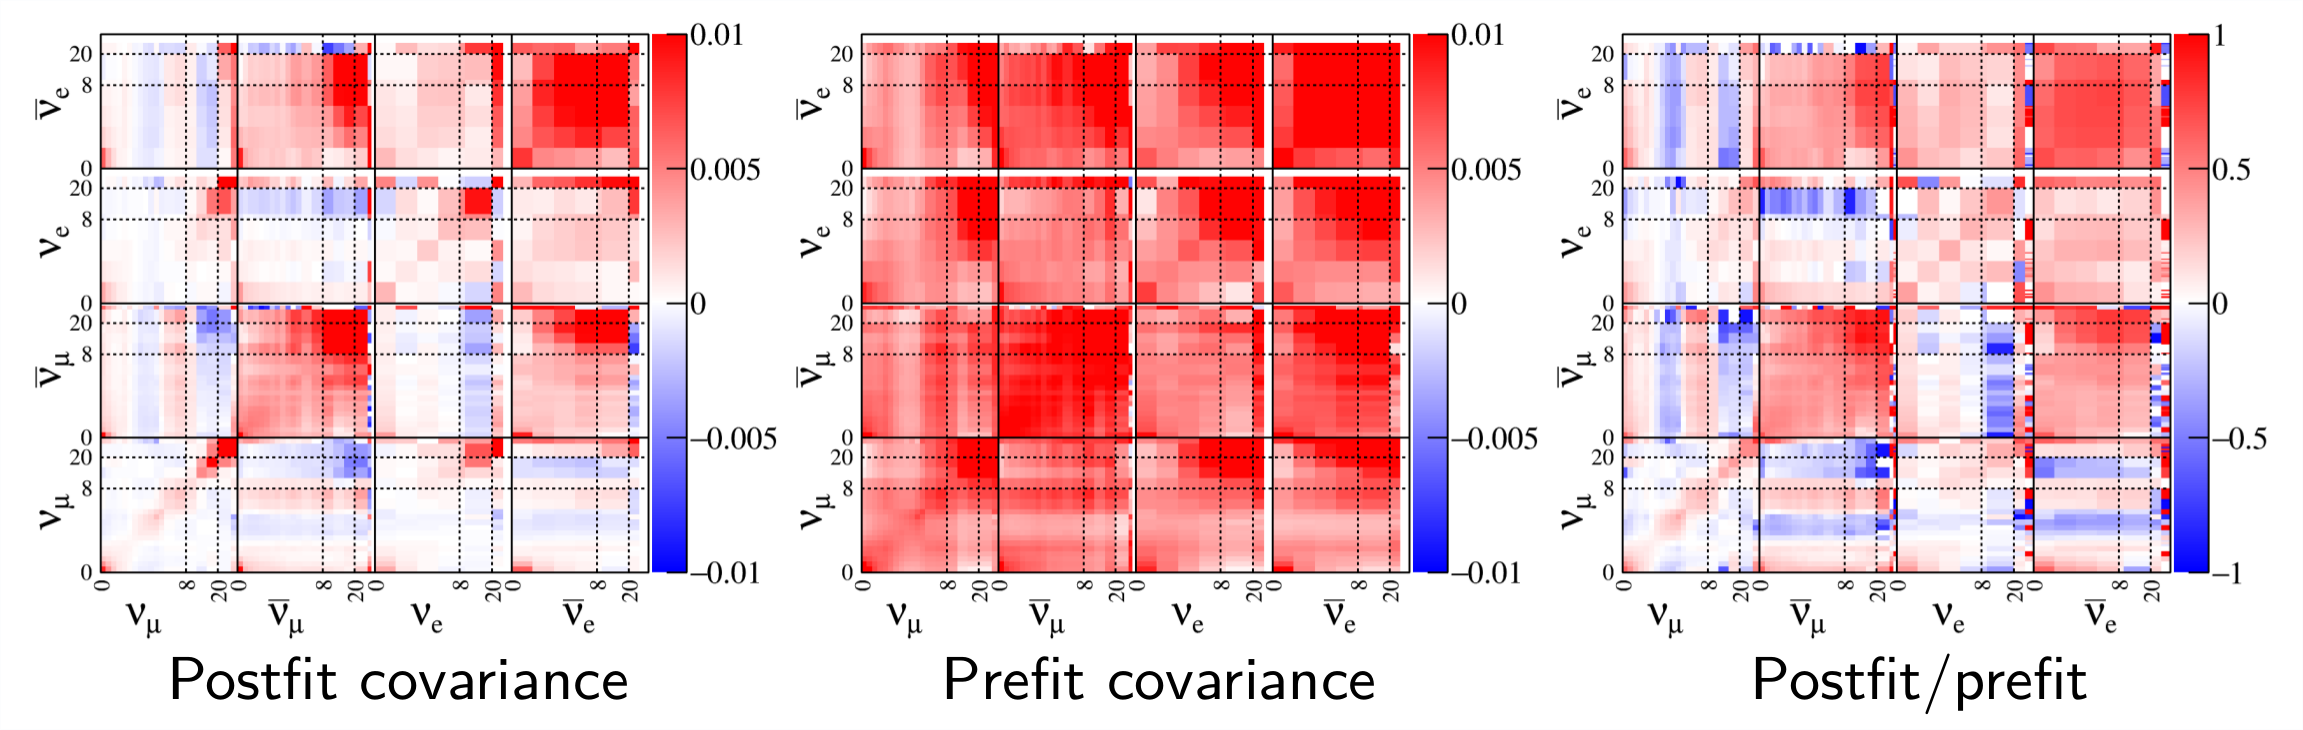
\includegraphics[width=\textwidth]{Figures/Covarience}
	\caption{Pre- and post-fit covariance matrices, along with a ratio of the two showing the extent to which correlations have been removed.}
	\label{fig:cov}
\end{figure}

The pre-fit and post-fit covariance matrices are shown in Figure~\ref{fig:cov}. 
The ratio of the pre- and post-fit shows the extent to which correlations are removed. 
The diagonal for $\nu_\mu$ is shown in Figure~\ref{fig:nue_con}, the shape-only constraint is extracted by normalizing the Monte Carlo to fake data and recalculating matrix. 

\begin{figure}[tbp]
	\centering
	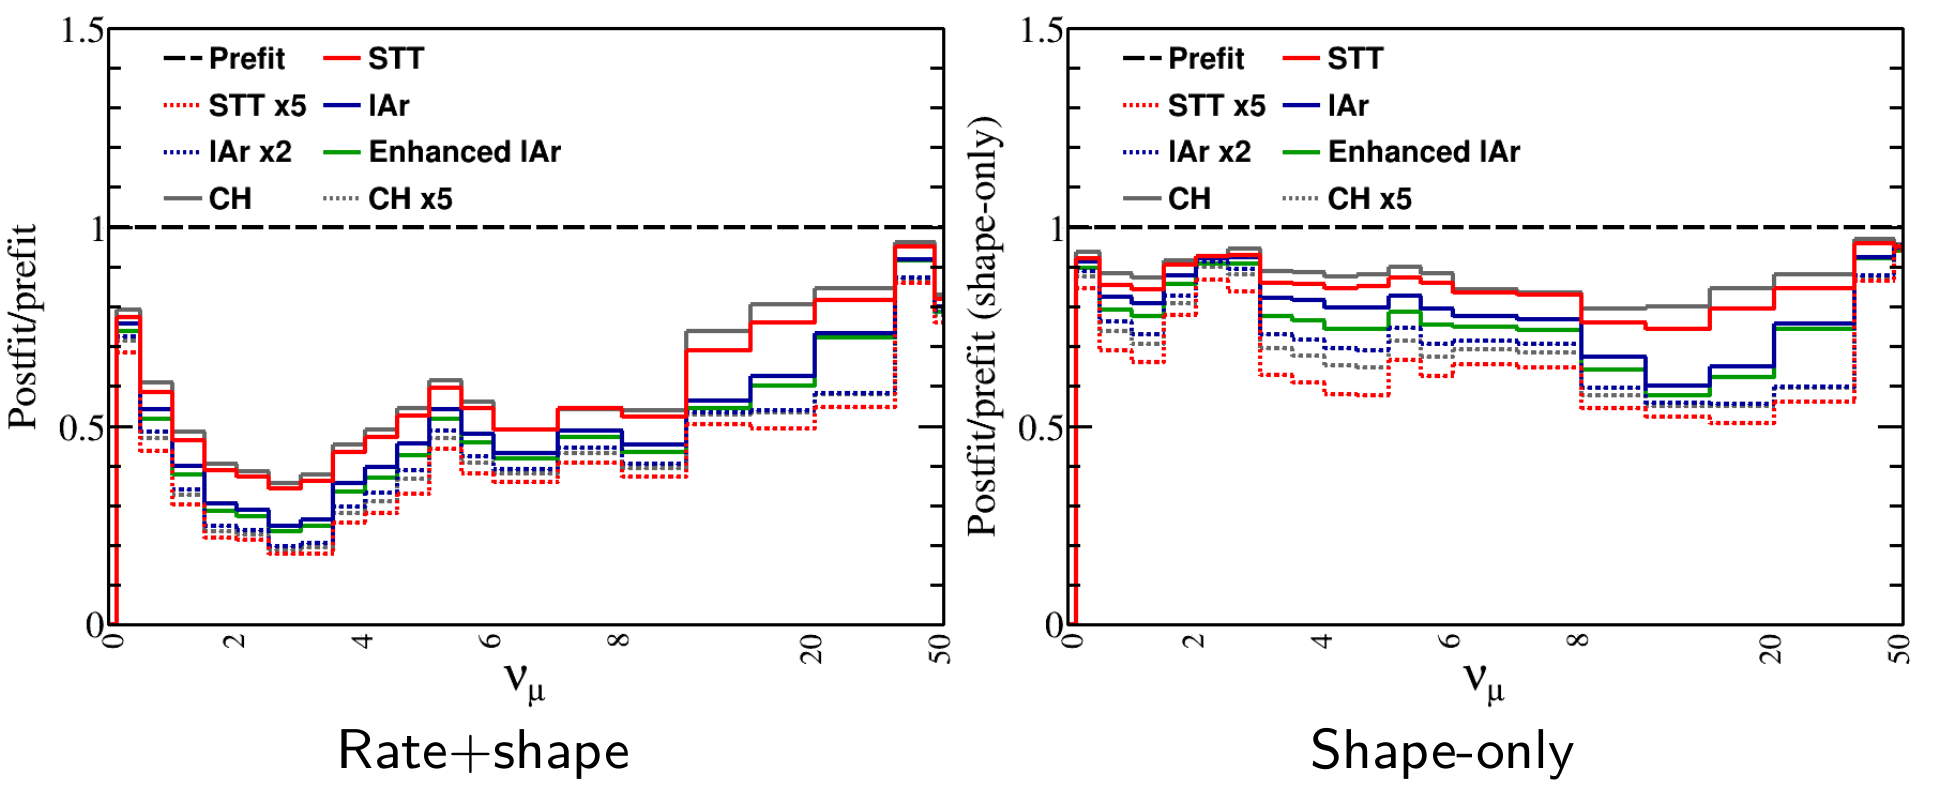
\includegraphics[width=\textwidth]{Figures/nue_conclusion}
	\caption{A diagonal of the post-fit covariance matrix shown in Figure~\ref{fig:cov}. SST is a 5~t Straw Tube Tracker. LAr is only a 15~t fiducial volume, with conservative angular resolution. Enhanced LAr has an optimized angular resolution.}
	\label{fig:nue_con}
\end{figure}

Figure~\ref{fig:nue_con} shows the $\nu$-$e^-$ ES technique a has potential to constrain the flux well.
Very little improvement is made at low-energy bins since the rate in this region is so low. 
The poor shape-only constraint is not a reflection on detector performance, but rather the strength of the constraint already applied by target models.
It was found that large mass and subsequently high rate are more important than angular resolution.
Hence, ArC has the potential to provide a flux constrain given the comparably high rates of $\nu$-$e^-$ ES.  

	
\section{Optimal Dimensions for Hadron Containment}\label{sec:had_containment}

The proposed ArgonCube dimensions are optimised for hadronic shower containment~\cite{lartpcSizeChris}. 
Showers are defined as contained if a reasonable efficiency across a wide range of kinematics is maintained, and there is no phase space with zero acceptance. 
The specific metric used is that \textgreater95\% of hadronic energy has to be contained, excluding neutrons and their descendants.

To assess the efficiency, detector volumes of varying sizes were simulated in a neutrino beam.
This provides a good measure of the efficiency of a given volume to contain different events, but it is not necessarily a good quantity to assess the required detector size.
Many events are not contained because of their specific location and/or orientation.
Cross-section coverage remedies this deficiency by looking at the actual extent of the event, instead of its containment, at a random position inside a realistic detector volume.
However, events extending through the full detector will very likely never be contained in a real detector due to the low probability of it exactly happening in the right location.
Therefore, the maximum event size needs to be selected smaller than the full detector size.
For the ND simulation this buffer was chosen as \SI{0.5}{\metre} in all directions.
Like this cross-section coverage allows to probe for phase space regions inaccessible to a particular detector volume configurations.

%%%princilple of variation 1 - startung 

While horizontal dimensions are unproblematic, the vertical \SI{3}{\metre} are at the lower limit.
According to the simulations, \SI{2.5}{\metre} would be sufficient but provide no safety margin at all.
Reducing the height by another \SI{0.25}{\metre} results in a significant loss of hadron containment already.
Figure~\ref{fig:dune-nd_lartpc-size} illustrates this by means of the cross-section coverage as a function of neutrino energy.
Cross-section coverage is similar to containment efficiency but should not be confused with the latter.


In Figure~\ref{fig:dune-nd_lartpc-size} it can be seen that cross-section coverage decreases rapidly for detector heights below \SI{2.5}{\metre}.
A height of \SI{3}{\metre} is therefore preferable to have some buffer for yet unknown uncertainties in the simulation.

\begin{figure}[tbp]
	\centering
	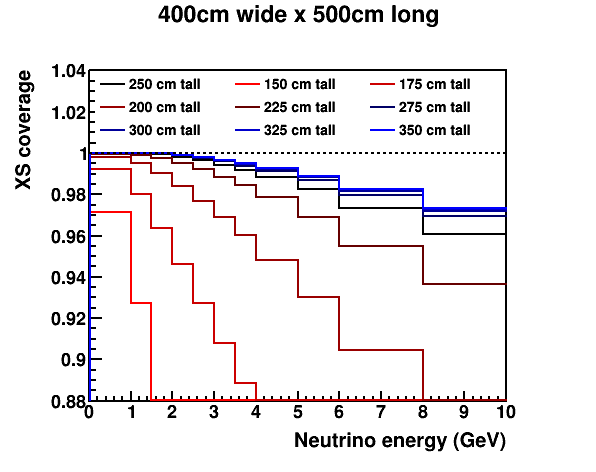
\includegraphics[width=\textwidth]{Figures/lartpc_size_vertical}
	\caption{Influence of the LArTPC size in the DUNE ND complex on hadron containment.
		Given in cross-section coverage as a function of neutrino energy.
		Horizontal dimensions are held constant at their nominal values of \SI{4 x 5}{\metre}.
		Height is indicated by colour.
		See text for explanation of cross-section coverage.~\cite{lartpcSizeChris}
	}
	\label{fig:dune-nd_lartpc-size}
\end{figure}

\subsection{Optimized Detector Dimensions}

\begin{figure}[tbp]
	\centering
	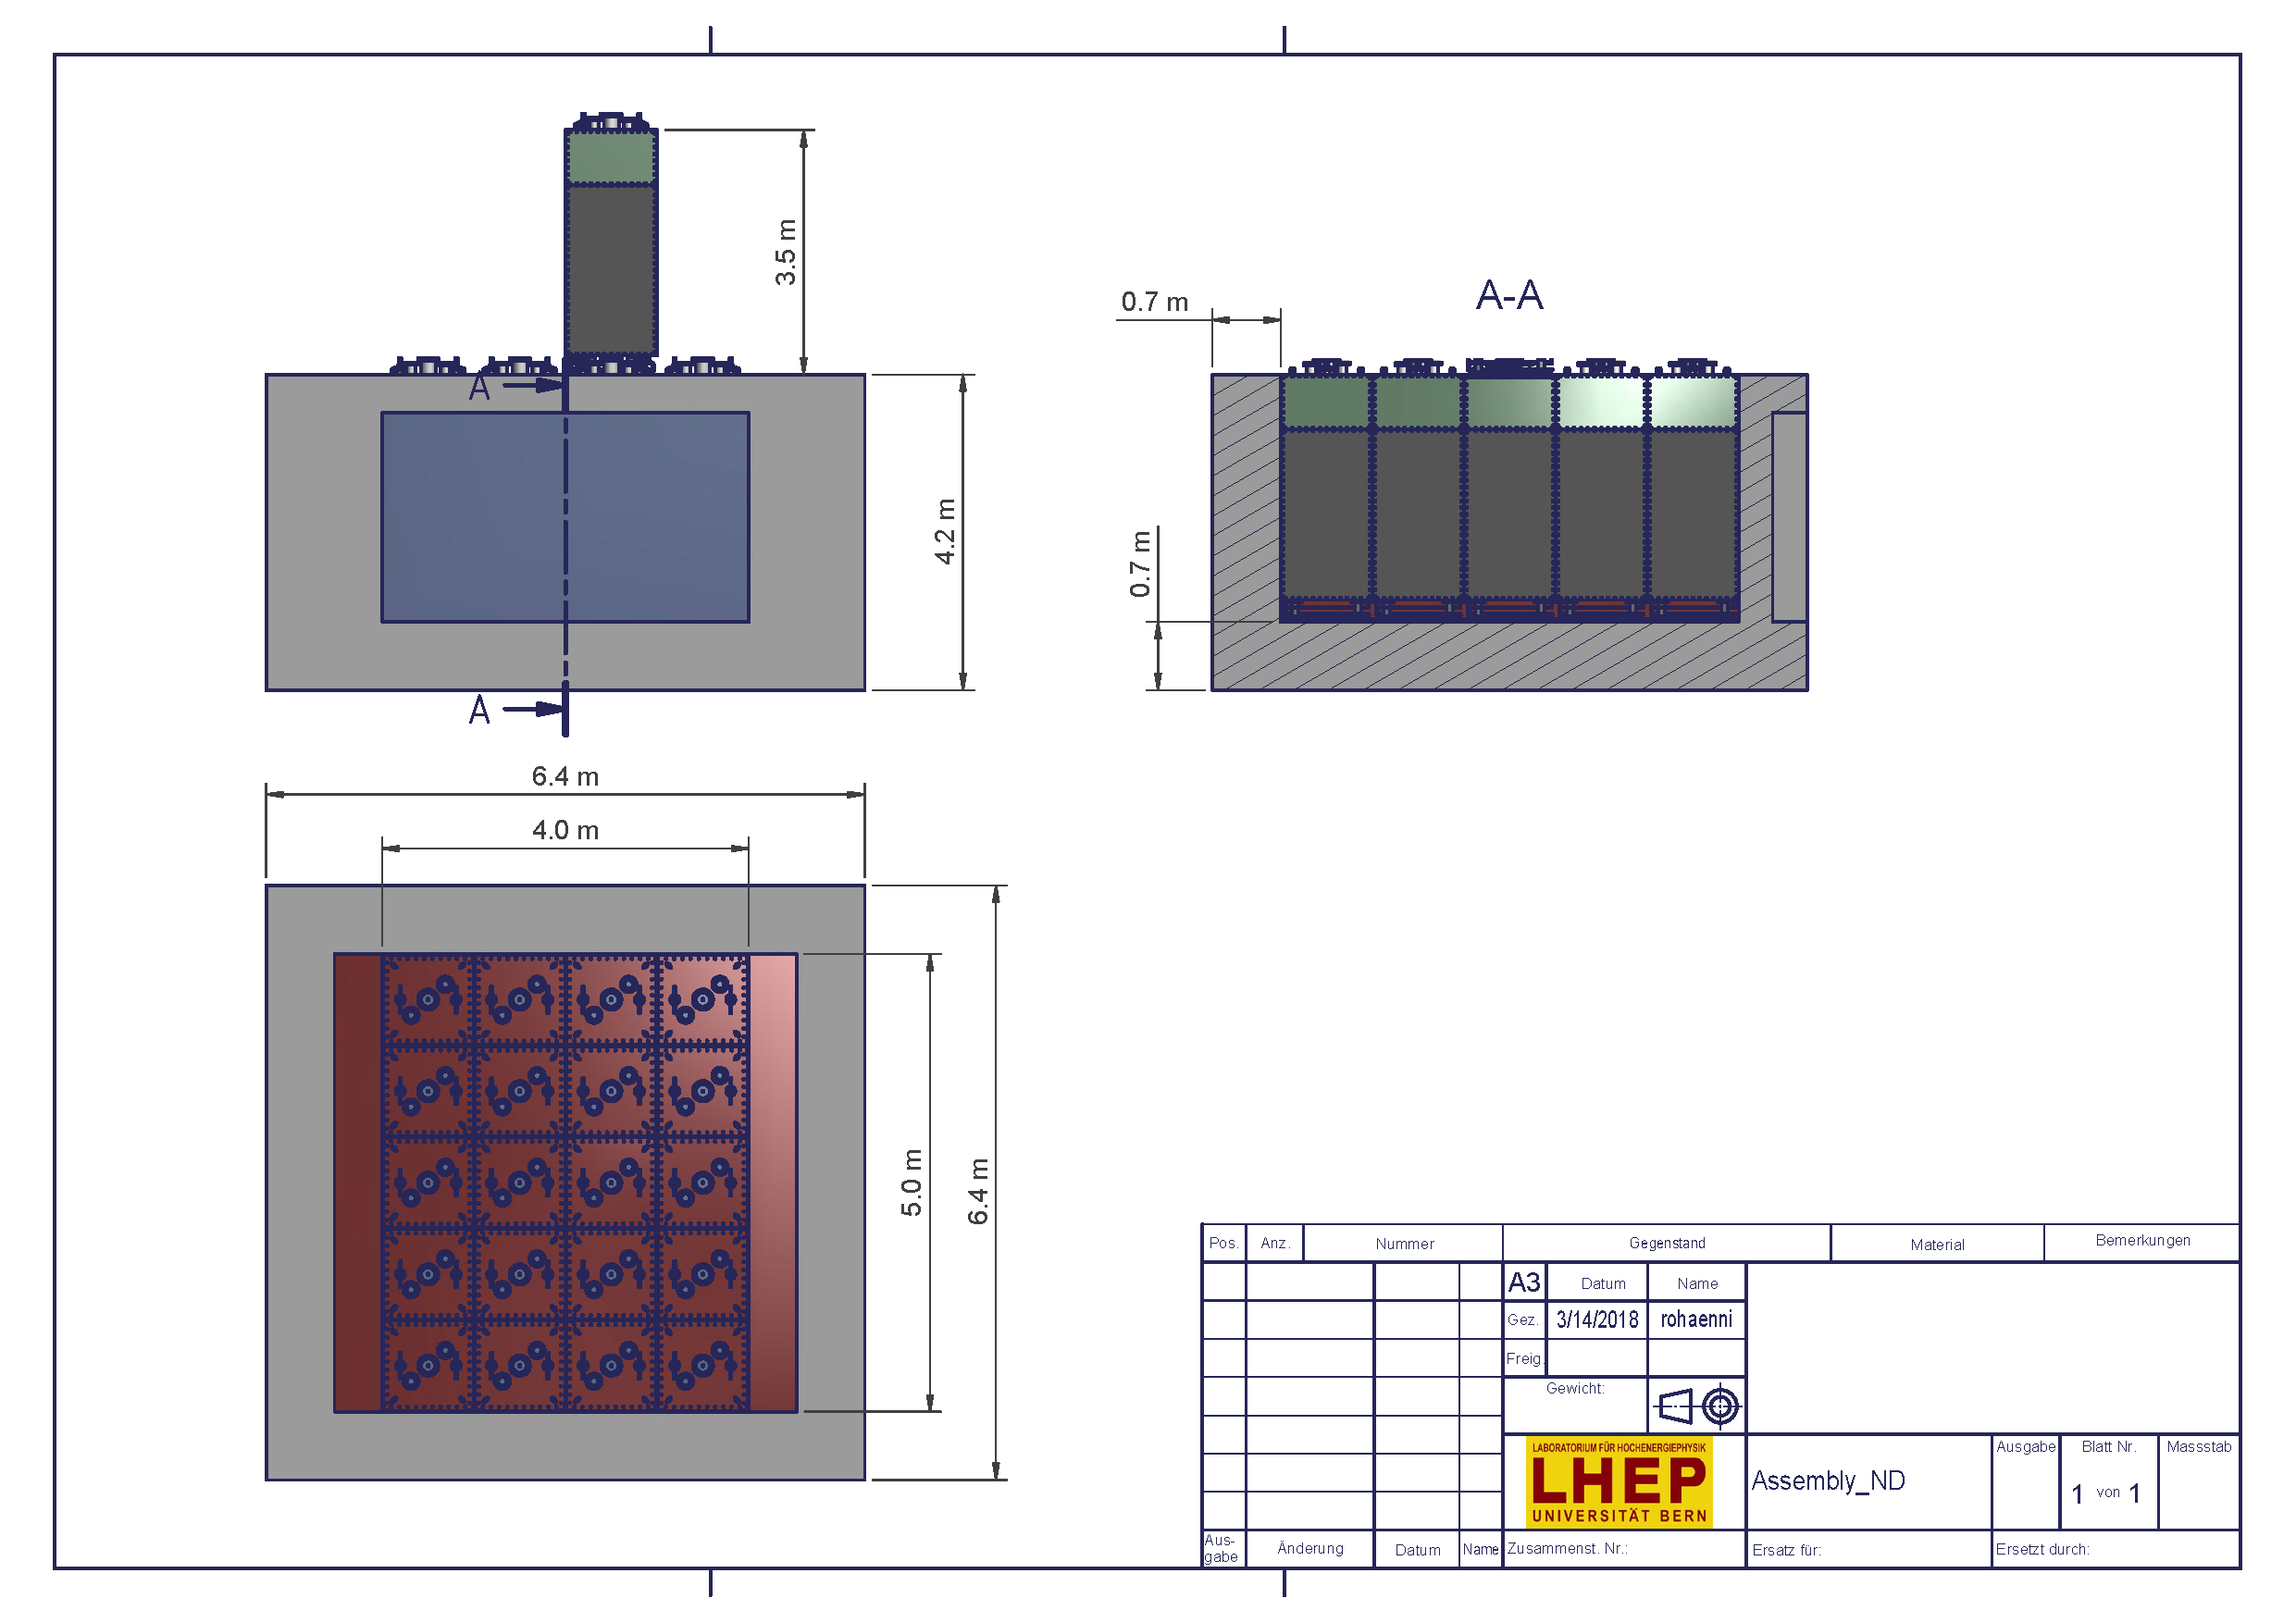
\includegraphics[width=\textwidth]{Figures/Assembly_ND-1}
	\caption{optimized geo design, using cryostat described in~\cite{gas}.}
	\label{fig:dune-nd_lartpc-size}
\end{figure}

\section{Muon Spectrometer Requirement}

\section{Statistics in Fiducial Volume}\label{sec:rates}

Rates are per bin. 37M total events per year in 25 t FV, FHC at 1.07 MW.

This is per year

Figure~\ref{fig:all_ey} is everything in the 25~t FV, contained is just the hadrons are contained.  Rates are per bin.  37M total events per year in 25t FHC at 1.07 MW.

\begin{figure}[tbp]
	\centering
	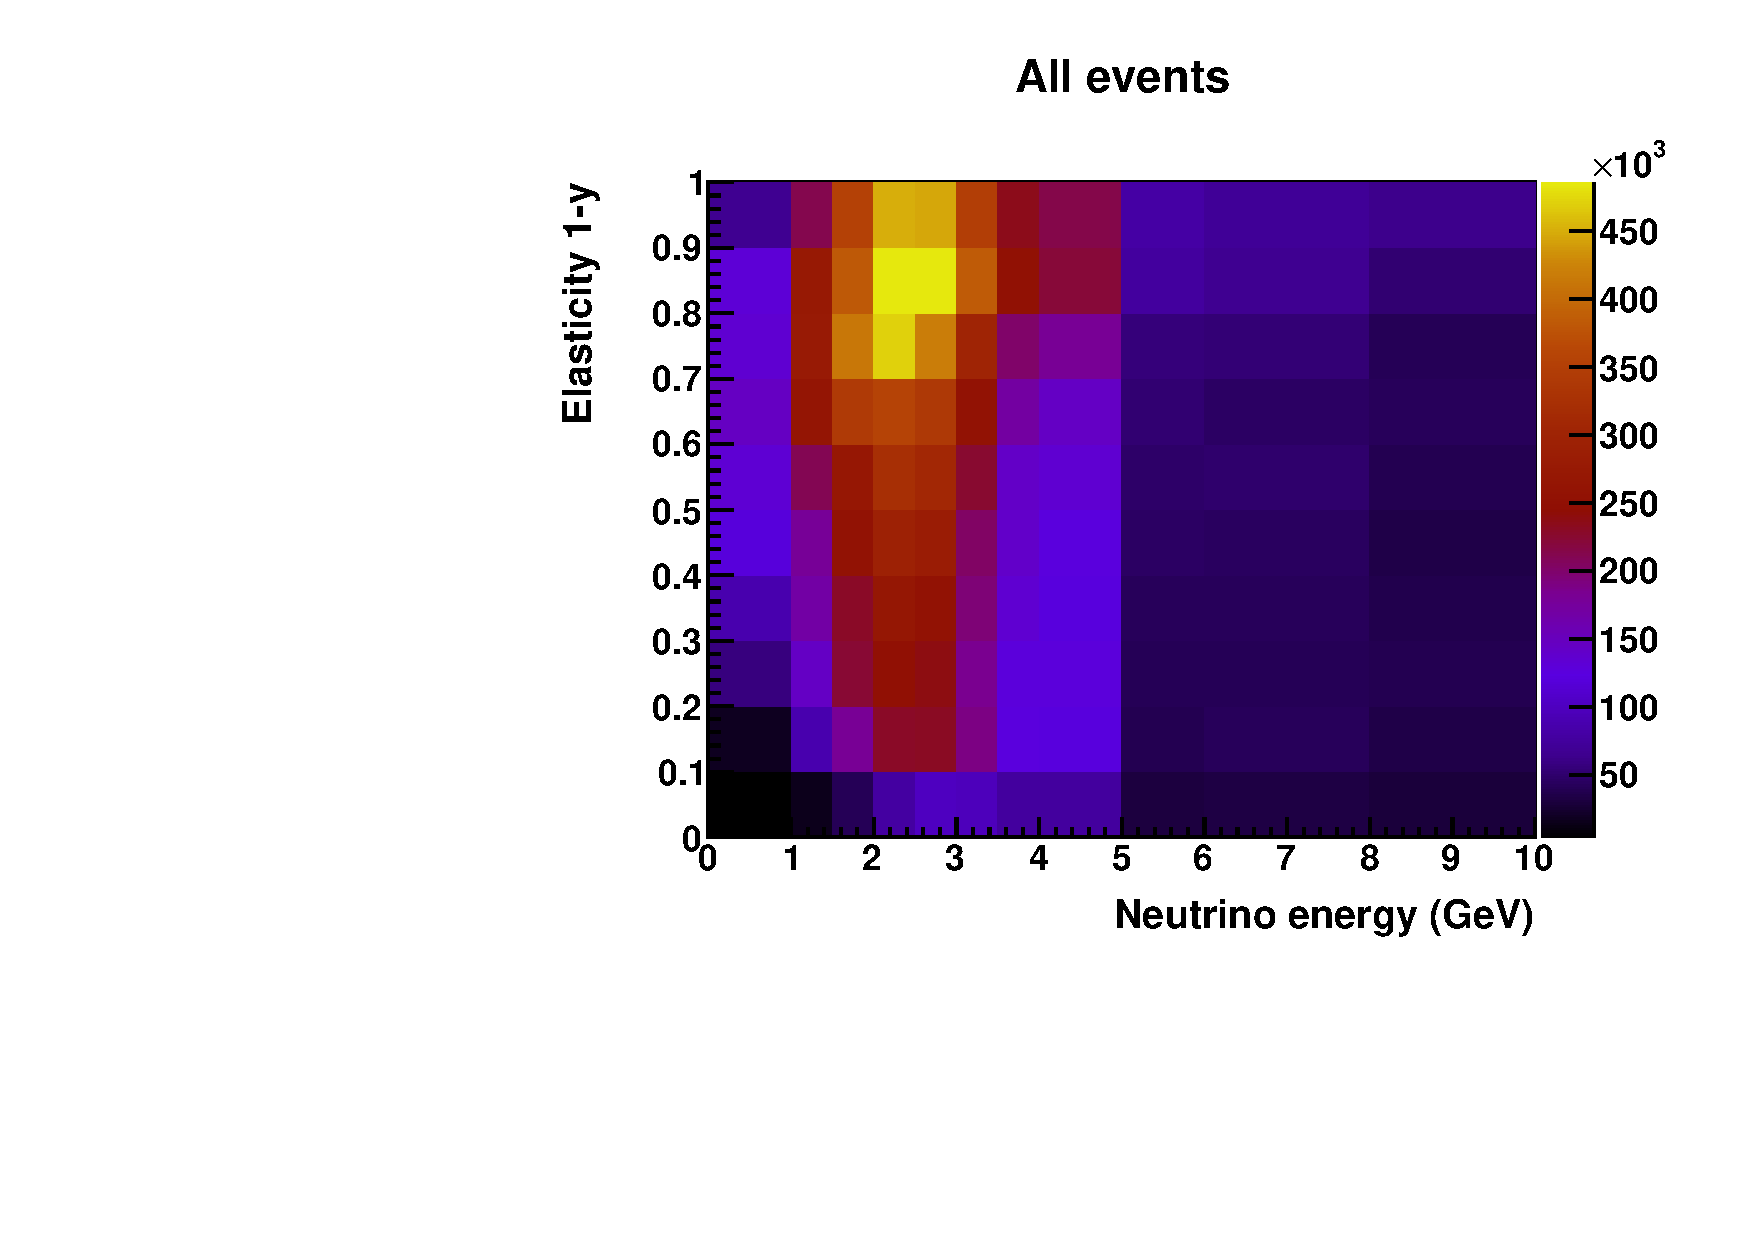
\includegraphics[width=\textwidth]{Figures/all_ey}
	\caption{all neutrino events in FV}
	\label{fig:all_ey}
\end{figure}

\begin{figure}[tbp]
	\centering
	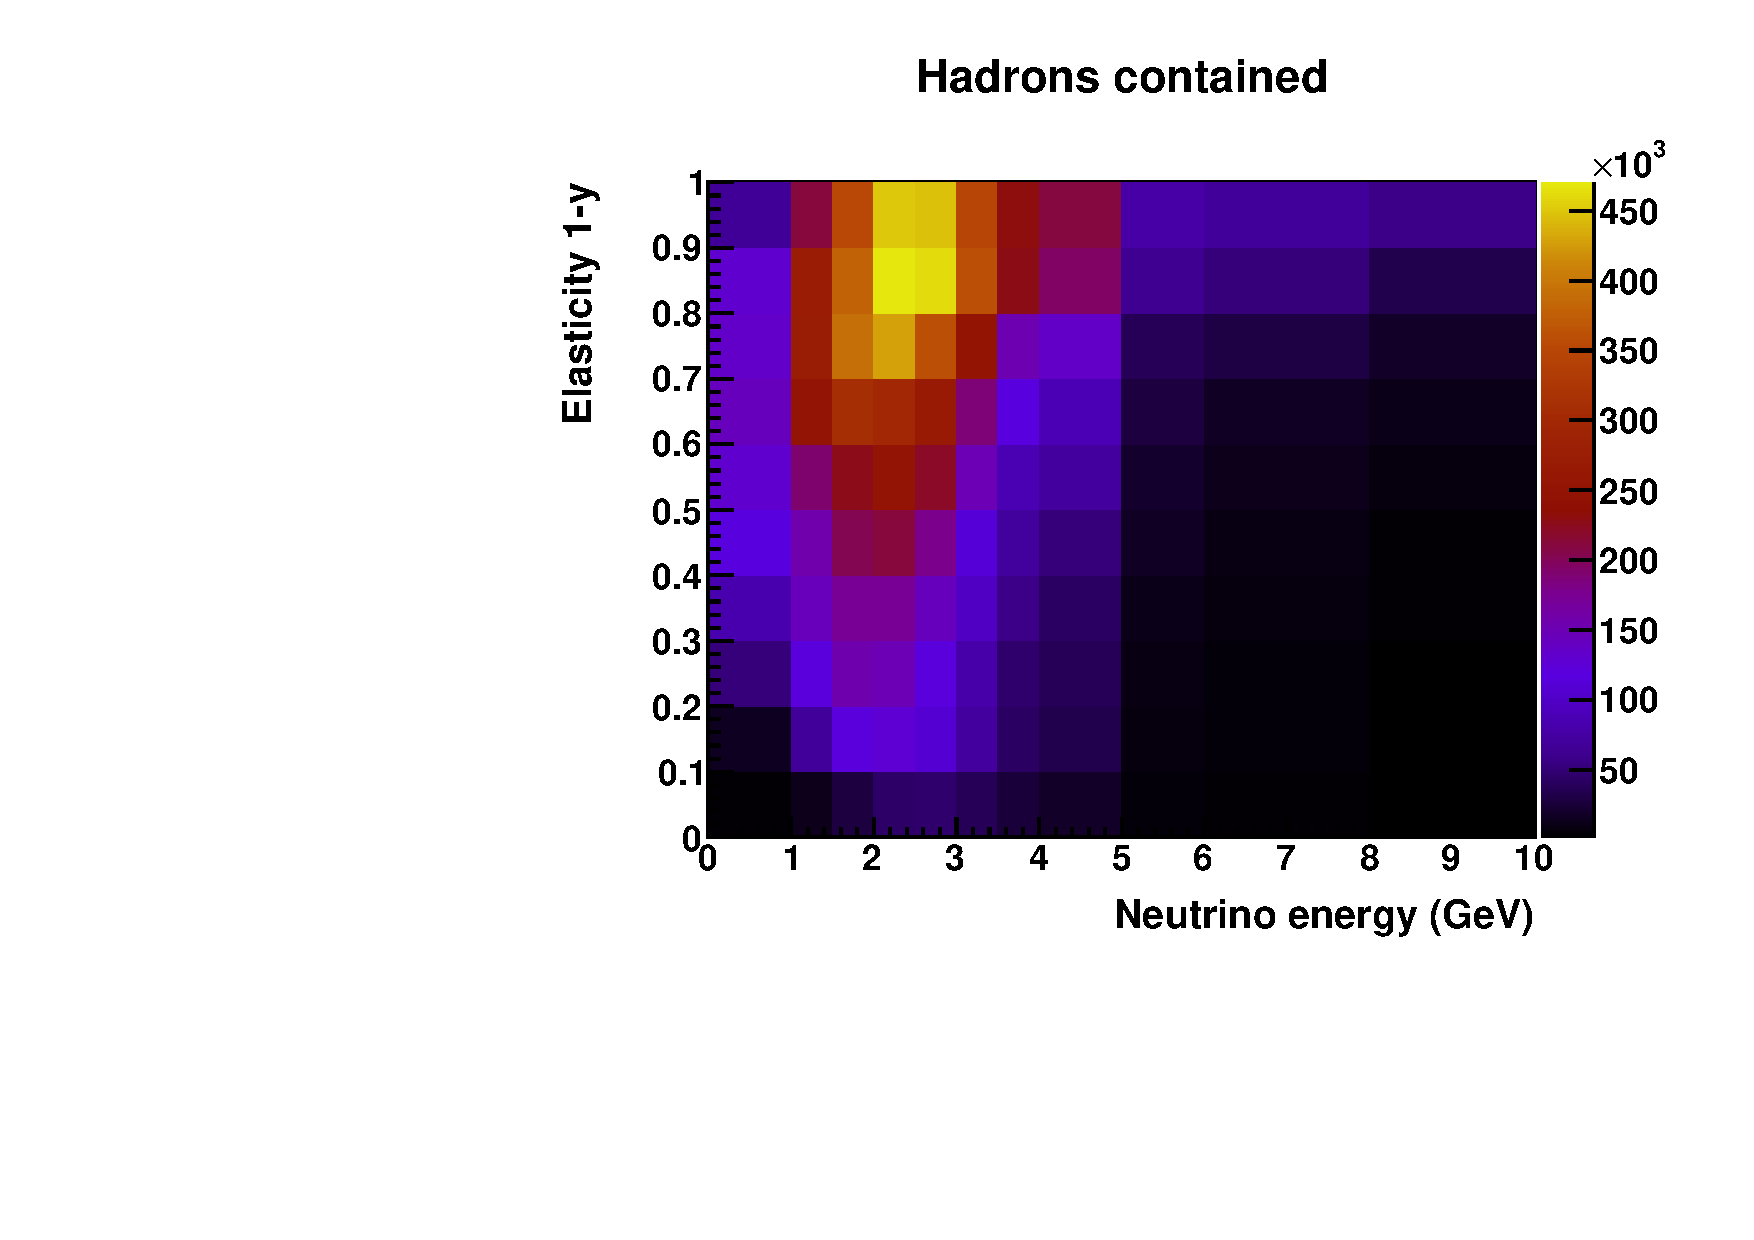
\includegraphics[width=\textwidth]{Figures/hadContNorm_ey}
	\caption{Contained hadrons in FV}
	\label{fig:hadContNorm_ey}
\end{figure}

\section{The Acceptance for Different Tracker Options}



\section{Muon and Electron Momentum Resolution and Scale Error}



This has not yet been investigated fully 

For muons, most of the momentum is measured in the downstream tracker.  The energy scale uncertainty from ArgonCube is basically a material model of LAr + passive materials.  It is hard to imagine getting the energy loss in LAr wrong in a systematic way; the passive materials is basically just how well the composition is known, which is probably \textless 1\%.

For electrons it is not as simple. The energy will be measured calorimetrically, not by range.  The MIP energy scale (Q/MeV) will be set by rock muons, but scaling it to more dense deposits from EM showers can bring uncertainties, i.e. recombination could be different.  So you'd like to do a test beam ideally.  We can get a nice sample of electrons up to 50 MeV from Michels of stopping rock muons. The $\pi^0$ invariant mass peak is another good standard candle.

\section{Can ArgonCube Measure Neutrons}


To minimise the stored energy, we have proposed segmenting the cathode and using field-shells to isolate individual TPCs, forming TPC modules. 
A further consequence of a modular detector volume is that the scintillation light is contained within each TPC module. 

If a dielectric light readout, such as ArCLight~\cite{arclight}, is deployed within the field-shells, this contained scintillation light can be efficiently measured with improved timing resolution.  
This makes the light readout system significantly more extensive than for a monolithic detector, and negates attenuation due to Rayleigh scattering at $6.6\times10^{-1}$~m~\cite{Rayleigh}.
It also improves trigger purity by providing a localised trigger, with minimal optical pileup.
The modular design lends itself to calorimetric measurements using the light readout.  

Scintillation light of LAr has prompt $<$\SI{6.2}{\nano\second} and slow \SI{1.3}{\micro\second}~\cite{scintillation} components, due to the lifetimes of the singlet and triplet states of the excimer molecules.
Optical pileup is due to overlapping of the slow component of the scintillation light from multiple interactions within the LAr, increasing the background light level throughout the detector.    
Optical pileup is intrinsically reduced by optically segmenting the detector.
Additionally, the slow component can be further suppressed by operating at higher electric fields~\cite{scintillationEfield}, effectively reducing the ionisation density~\cite{scintillationdEdx}. 

Studies have shown that the contained prompt scintillation light provides an important handle for neutron tagging, by associating detached energy deposits to the correct neutrino interaction using timing information. 
Figure~\ref{fig:NDSpill} shows a simulated beam spill in the \SI[product-units=repeat]{5x4x3}{\metre} LAr component of the DUNE ND. 
It highlights the problem of associating fast-neutron induced energy deposits to a neutrino vertex using only collected charge.  

\begin{figure}[htb]
	\centering{
		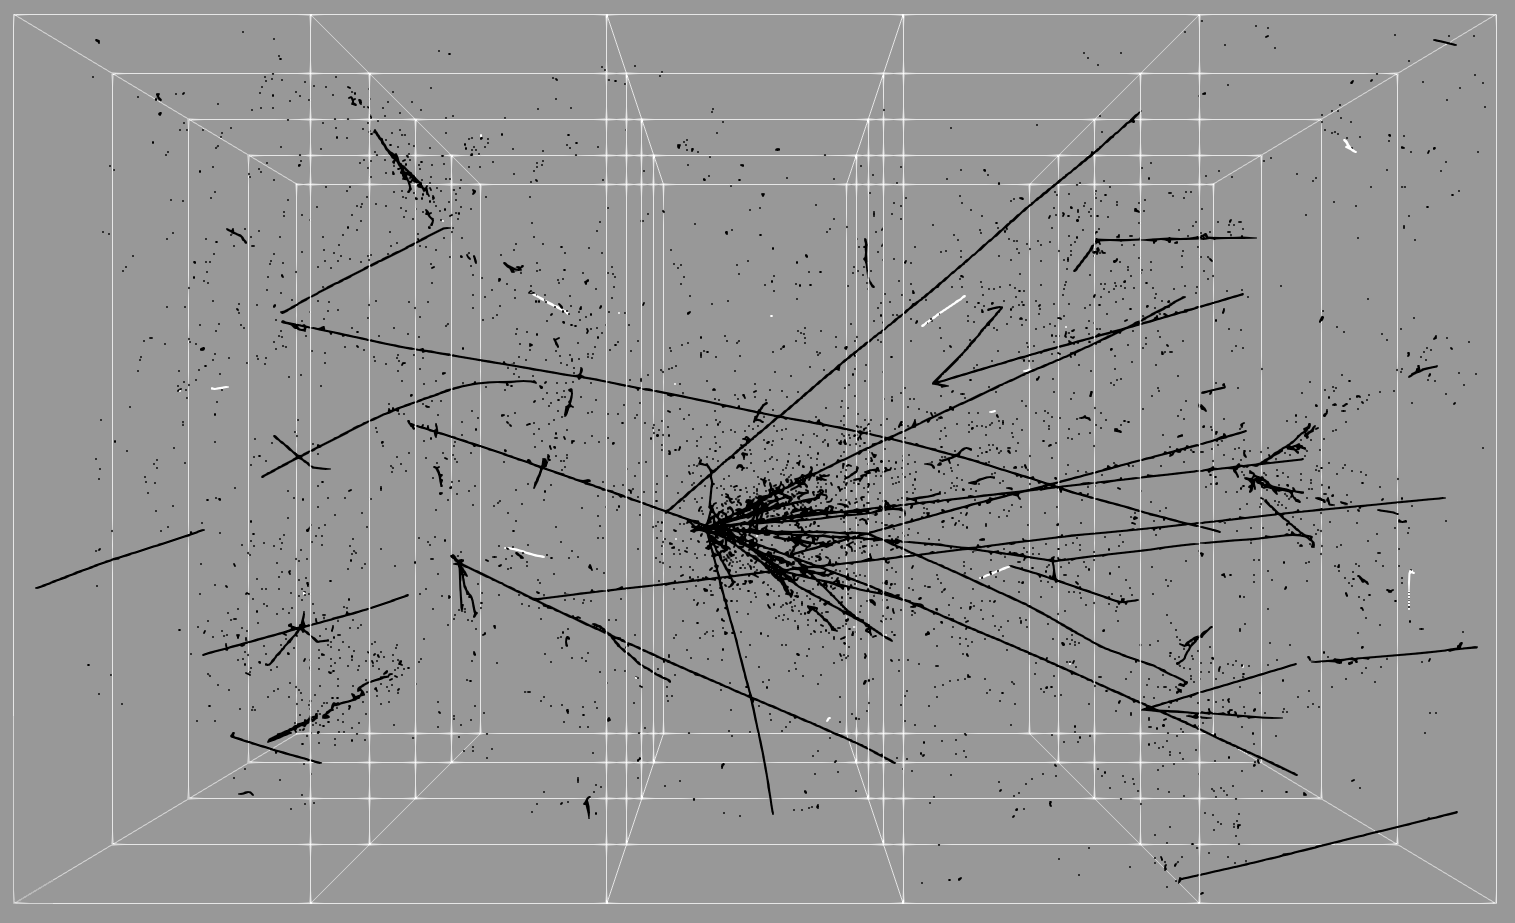
\includegraphics[width=.97\textwidth]{Figures/NeutronNDSpill.png}
	}
	\caption{A beam spill in the LAr component of the DUNE ND. 
		The detector volume is \SI[product-units=repeat]{5x4x3}{\metre}.
		Fast-neutron induced recoiling proton tracks, with an energy threshold greater than $\sim\,$\SI{10}{\mega\electronvolt}, are shown in white.
		The black tracks are all other energy deposits sufficient to cause charge collected at the pixel planes.}
	\label{fig:NDSpill}
\end{figure}


By containing scintillation light, prompt light signals can be used to associate fast-neutron induced deposits back to a neutrino vertex anywhere within the detector.
Figure~\ref{fig:Timing} shows the temporal distribution of neutrino vertices within a beam spill.
The mean separation of neutrino vertices is \SI{279}{\nano\second}, with all fast-neutron induced energy deposits occurring $<$\SI{10}{\nano\second} after each neutrino interaction.      

\begin{figure}[htb]
	\centering{
		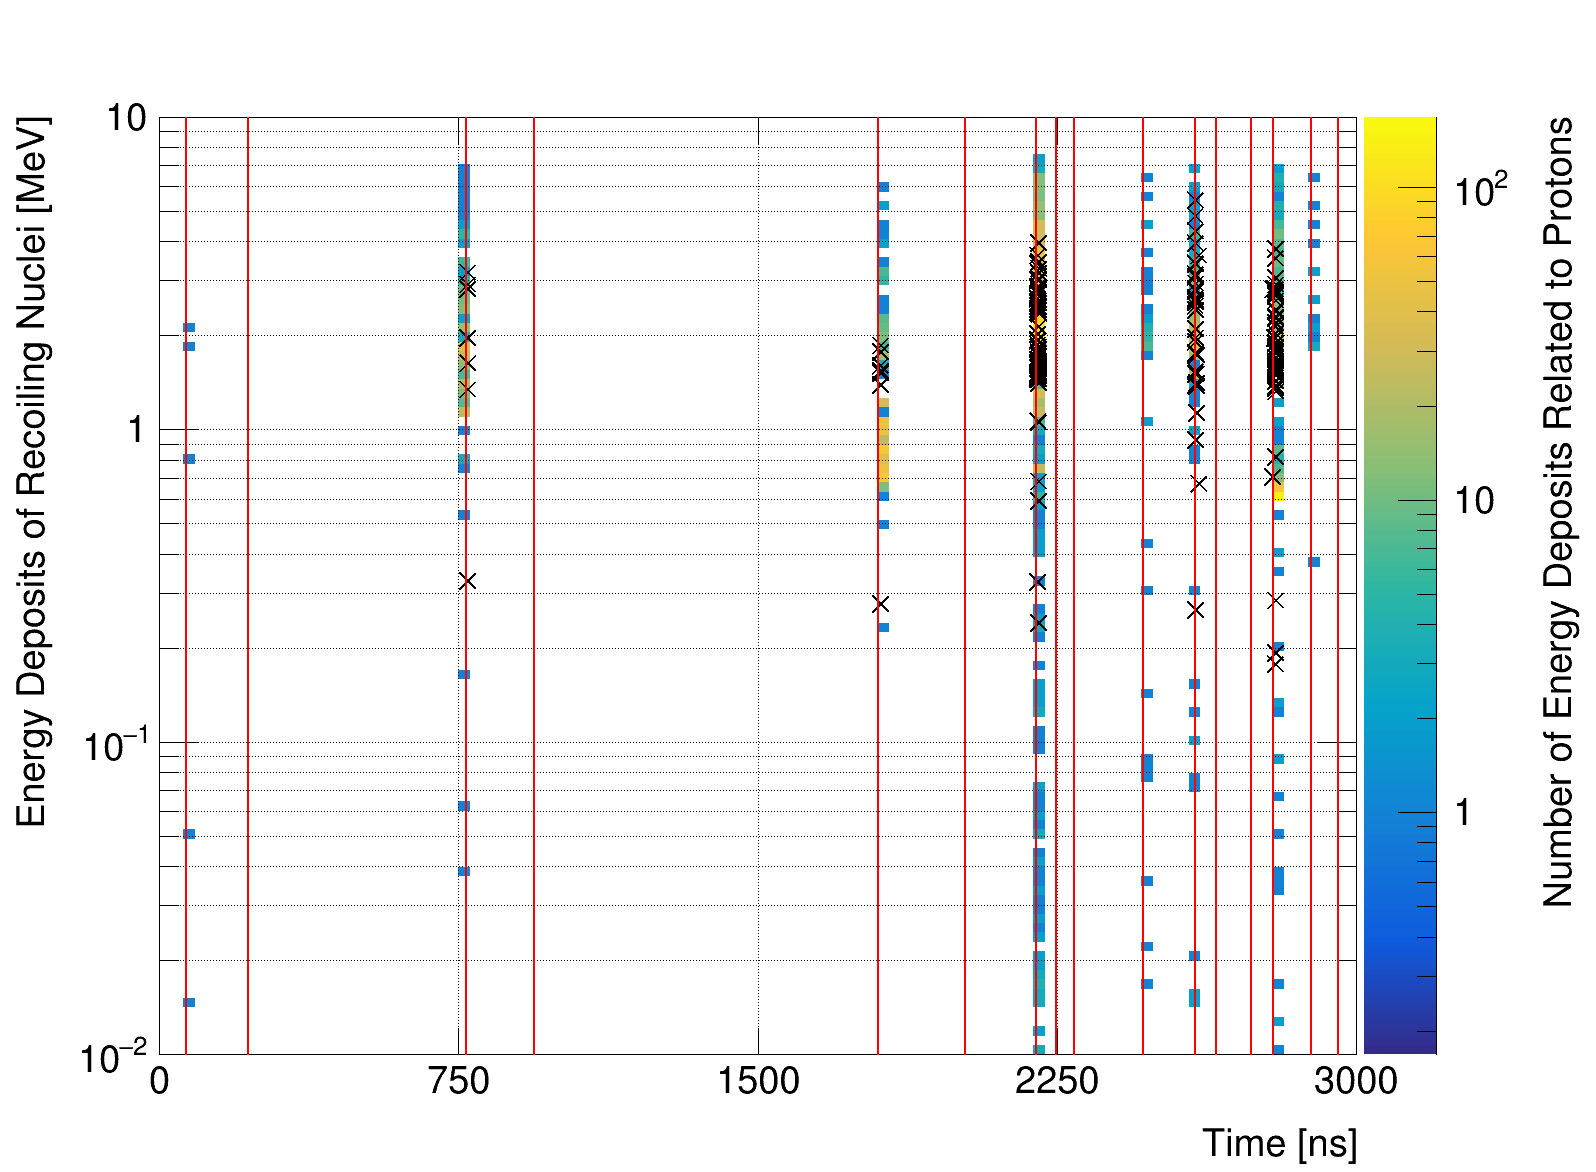
\includegraphics[width=.97\textwidth]{Figures/recoil_proton_edep_vs_vtx_time_a.png}
	}
	\caption{The temporal distribution of neutrino vertices (red lines) within a beam spill in the LAr component of DUNE ND.
		The mean separation of neutrino vertices is \SI{279}{\nano\second}. The filled bins show the number of hits due to recoiling protons, crosses indicate a hit due to a recoiling $^{2}$H, $^3$H, $^2$He or $^3$He nucleus.
		All fast-neutron induced energy deposits occur $<$\SI{10}{\nano\second} after each neutrino interaction.}
	\label{fig:Timing}
\end{figure}

A better handle on neutron tagging is important in order to minimise the uncertainty on neutrino energy reconstruction.
Not only for neutrons generated at a neutrino vertex, but also for hadronic showers that fluctuate to neutrons leading to detached energy deposits of $\mathcal{O}\left(10\right)\,\mathrm{MeV}$.   
Improved light collection efficiency and timing resolution are also likely to help DUNE's low energy physics programme. In particular, the detection efficiency for low momentum kaons produced by DUNE's headline proton decay channel $p\rightarrow K^{+} + \bar{\nu}$ should be significantly improved by the improved light collection.

	
	\printbibliography
	
\end{document}



  
